\clearpage
%\begin{savequote}[8cm]
%\textlatin{Neque porro quisquam est qui dolorem ipsum quia dolor sit amet, consectetur, adipisci velit...}
%
%There is no one who loves pain itself, who seeks after it and wants to have it, simply because it is pain...
%  \qauthor{--- Cicero's \textit{de Finibus Bonorum et Malorum}}
%\end{savequote}

\chapter{\label{ch:5-cpfit}Fits for \CP observables in two- and four-body decays} 

\minitoc

In this section the \CP observables are measured by performing a fit to \btodkst candidates in data simultaneously for each \Dz decay mode for both \Bp and \Bm decays. This fit is referred to in this thesis as the \CP fit. The setup of the \CP fit is outlined in Section \ref{sec:cpfit:setup}, followed by the fit results in Section \ref{sec:cpfit:results}. Section \ref{sec:systematics} outlines the systematic uncertainties and the results of the \CP observables are summarised in Section \ref{sec:cpfit:summary}.

\section{Setup of \CP fit}
\label{sec:cpfit:setup}

The fit to data is performed on the invariant mass of \btodkst candidates. A simultaneous fit strategy is employed to fit each of the \Dz decay modes as well as two bins of \B charge (\Bp and \Bm), two bins of \KS reconstruction type (LL and DD) and two bins of data type (\runone and \runtwo), resulting in 56 bins in total. The parameters extracted from this simultaneous fit are the \CP observables, namely \Akpi, \Akk, \Apipi, \Rkk, \Rpipi, \Rptwo, \Rmtwo, \Akpipipi, \Apipipipi, \Rpipipipi, \Rpfour and \Rmfour, which relate to the physics parameters of interest as shown in Equations \ref{exp_Acp} - \ref{exp_R4pi}.

The simultaneous fit extracts the \CP observables directly, rather than measuring the pure yields and indirectly converting them into the \CP observables. The strategy to extract the \CP observables directly avoids the need to deal with combining results from different categories, which is complicated due to the many correlations between the variables. This strategy also leaves fewer fit parameters to be dealt with. This simultaneous fit, which extracts the \CP observables, is referred to in this thesis as the \CP fit. The reason for performing a simultaneous fit is that the \CP observables being measured relate to the ratios of yields in different \Dz modes and different \B meson charges, therefore it is necessary to perform a fit that includes separate data samples associated with each of the modes and charges. Additionally, some shape parameters are found to be different in the different in different bins of \KS reconstruction type and data-taking period, and a simultaneous fit allows these differences to be easily dealt with. 

This section covers the setup of the \CP fit. The components and shapes of the \CP fit are the identical to those described in Section \ref{sec:massfit}, with the exception of and additional component in the \kk mass spectrum, detailed in Section \ref{sec:cpfit:Lb2LcKst}.


%The mean and width of the signal shape are shared across the different run periods and across modes of the same number of final state particles, but the mean and width are allowed to be different for the two- and four-body modes. The shape and yield of the partially reconstructed background is completely fixed, with different shape parameters for LL and DD candidates. The shape is fixed as described in Section \ref{sec:massfit:partreco}, using the yield ratios given in Table \ref{fixedyieldratios}. The total partially reconstructed yield is fixed from the fits in Figures \ref{massfitskpi} and \ref{massfitsk3pi}, the values for the total partially reconstructed yield in each of the simultaneous fit categories is given in Section \ref{sec:cpfit:partrecoyields}. The shape of the combinatoric background is shared across all modes of the same number of final state particles, but has different values for LL and DD candidates, as well as two and four-body D modes.

\subsection{Additional background component in \kk mass spectrum}
\label{sec:cpfit:Lb2LcKst}

The mass fit model described in Section \ref{sec:massfit} is used to model all \Dz modes in the \CP fit, however, there is an additional source of background included in the \kk model that does not occur in the other modes. This background in the \kk \Bm mass spectrum comes from the decay \decay{\Lb}{\Lc(p\Km\pip)\Kstarm}, where the proton is misidentified as a kaon and the \pion is missed in the reconstruction. The decay mode \decay{\Lc}{p\Km\pip} accounts for over 6\% of the \Lc branching fraction~\cite{PDG2016}, whereas \Lc decays that may contribute as background to the other \Dz decay modes, e.g. \decay{\Lc}{p\pim\pip}, are suppressed by an order of magnitude. Therefore, this background is only considered for the \kk decay model.

The shape used to model this \decay{\Lb}{\Lc(p\Km\pip)\Kstarm} contribution is a Cruijff function, defined as,
\begin{equation}
  \mathrm{Cruijff}(m; \mu,\sigma_L,\sigma_R,\alpha_L,\alpha_R)=
\begin{cases}
    exp \left( -\frac{(m-\mu)^2}{2\sigma_L^2 + \alpha_L(m-\mu)^2} \right) ,     & \text{if } m-\mu < 0, \\
    exp \left( -\frac{(m-\mu)^2}{2\sigma_R^2 + \alpha_R(m-\mu)^2} \right) ,     & \text{otherwise.}
\end{cases}
\label{Cruijff}
\end{equation}%
where $\mu$ is the peak position, $\sigma_{L,R}$ is the width on the left and right sides of the peak and $\alpha_{L,R}$ is a modification constant. The shape parameters can be taken from using a simulated sample of \decay{\Lc}{p\Km\pip} events, reconstructed as \decay{\Bm}{\D\Kstarm} signal events, and performing a fit to the \Bm mass distribution. However, due to reasons relating to timing and speed of generation, a simulated sample of \decay{\Lc}{p\Km\pip} events was not available. Instead, the shape parameters are taken from a fit to a simulated sample of \decay{\Lb}{\Lc\Km} events reconstructed as \decay{\Bm}{\D\Km} events; this shape is expected to be similar to \decay{\Lc}{p\Km\pip}, and any uncertainty in the shape is accounted for as a systematic uncertainty, described in Section \ref{sec:systematics}.

The fit to the \Bm mass spectrum is shown in Figure \ref{Lbfit}, where it can be seen that the reconstructed \Bm mass falls between 4800 and 5500 \mevcc, and the results from this fit are shown in Table \ref{fitresultsLb}. All the values for the shape parameters are fixed in the simultaneous fit to the values in Table \ref{fitresultsLb}; these fixed values are considered to be a source of systematic uncertainty, detailed in Section \ref{sec:systematics}. 

\begin{figure}[h]
\centering
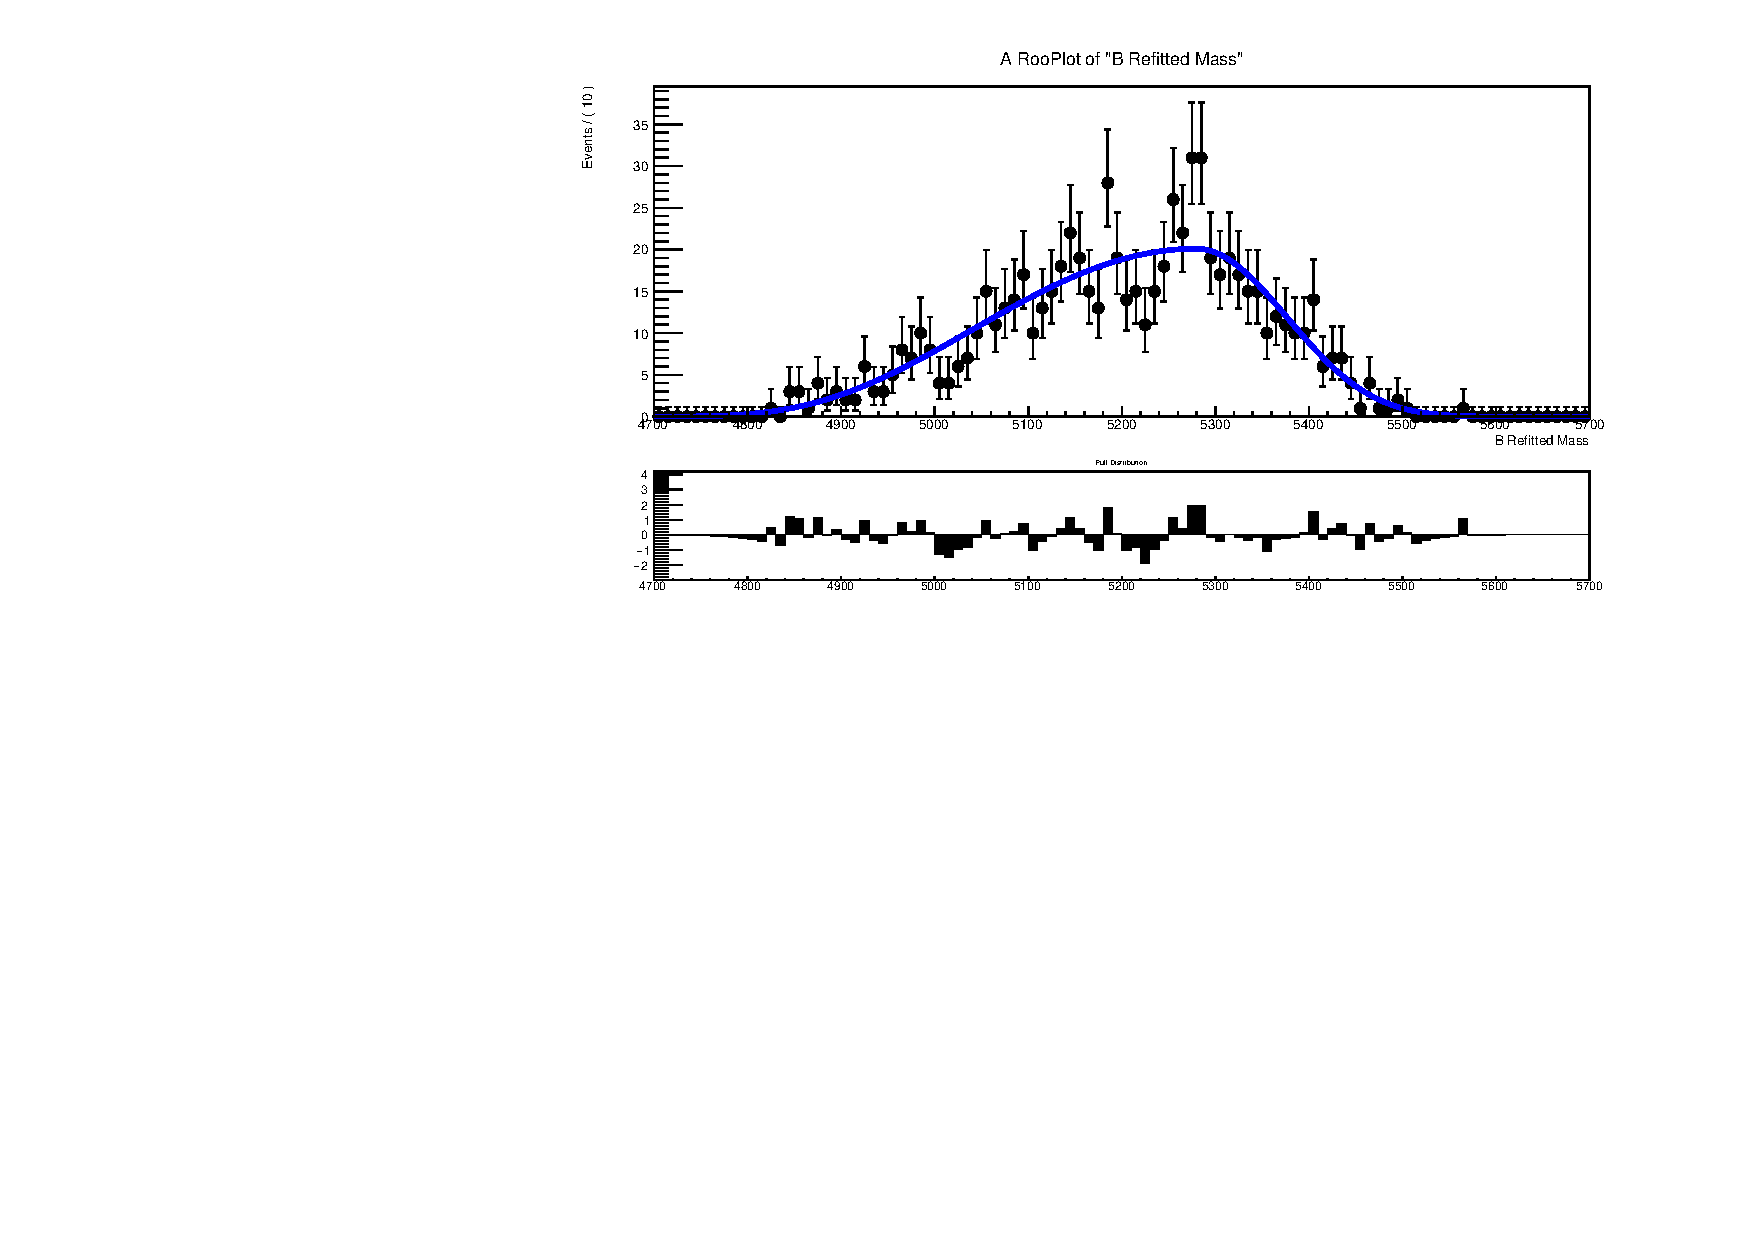
\includegraphics[width=0.7\linewidth]{figures/backgrounds/Lb2LcKst.pdf}
\caption{Fit to distribution of simulated \decay{\Lb}{\Lc(p\Km\pip)\Km} sample using a Cruijff function, where the \pip is missed in reconstruction and the proton is misidentified as a kaon. This contributes as a source of background in the \decay{\Bm}{\D\Kstarm}, \decay{\D}{\Kp\Km} fit.}
\label{Lbfit}
\end{figure}

\begin{table}[h]
\centering
\begin{tabular}{cc}
\hline
Parameter & Value \\
\hline
$\mu$ & $5280 \pm 18$ \\
$\sigma_L$ & $221 \pm 26$ \\
$\sigma_R$ & $96 \pm 16$ \\
$\alpha_L$ & $-0.19 \pm 0.19$ \\
$\alpha_R$ & $-0.04 \pm 0.06$ \\
\hline
\end{tabular}
\caption{Shape parameters from a fit to simulated \decay{\Lb}{\Lc\Km} events using a Cruijff function. These shape parameters are fixed with an associated systematic uncertainty.}
\label{fitresultsLb}
\end{table}

The shape is assumed to be the same in each \kk fit category, across \KS reconstruction types and data-taking periods because there is such a low number of events that contribute to this background that the possible variations in the shape in these different categories has negligible effect on the results. The \decay{\Lb}{\Lc(p\kaon\pi)\Kstarm} yield compared to the signal yield in the favoured \kpi mode is allowed to vary in the simultaneous fit. This fractional yield is required to be the same for all fit categories.

%%%%%%%%%%%%%%%%%%%%%%%%
\subsection{Choice of fit range}
\label{sec:cpfit:range}	

Fixing the relative yields for the partially reconstructed shapes, as described in Section \ref{sec:massfit:partreco}, assumes that no \CP violation occurs, i.e. the relative yields for \Bm and \Bp are the same. This is a reasonable assumption for the favoured \kpi and \kpipipi decays considered in this section, where we do not expect \CP violation. However in the other \D final states, for example \pik, \CP violation is expected in the partially reconstructed background for which the \CP violation parameters are not known. Therefore, it is not possible make any constraints on the yield ratios in these modes. The fit that would result from fitting six individual yields with an order of magnitude less data would be unstable and this lack of constraint in the low mass region would lead to a large amount of freedom in the combinatorial, significantly affecting the precision of the signal yield. 

The overlap of the partially reconstructed and signal peaks is very small. There are a number of advantages to raising the lower range of the mass parameterisation up to 5230 \mev, which only removes 0.4\% of signal. The advantages include avoiding the need to fit the various partially reconstructed yields in each of the other D decays modes. These cannot use the same assumptions and fractions as determined in the Cabibbo-favoured mode due to expected CP violation. Further benefits are that low level broad backgrounds that may be present in the range 4900 - 5200 \mev do not need to considered as sources of systematics uncertainty. The shape and yield of the small amount of partially reconstructed background present in all \D decay categories above 5230 \mev is determined and fixed from the fits to data of the \kpi and \kpipipi decays, taking into account the smaller branching fractions of the \D decays. It is less than an event for all the CP violating modes. Due to the assumptions present in the initial fit, uncertainties in the yield and shape and possible asymmetries in distribution between \Bp and \Bm are evaluated as systematic uncertainties. This systematic uncertainty is dealt with in Section \ref{sec:systematics:partreco}.

\subsection{Partially reconstructed yield in \CP fit}
\label{sec:cpfit:partrecoyields}

The modelling of the partially reconstructed background is described in detail in Section \ref{sec:massfit:partreco}. As discussed in Section \ref{sec:cpfit:range}, the low mass limit in the \CP fit is 5230\mevcc, which removes almost all of the partially reconstructed background. The \CP fit fully fixes the shape and yield of the partially reconstructed background in each of the different \Dz modes. Table \ref{partrecofixedyields} shows the fixed values of the total partially reconstructed yield in the \CP fit.

\begin{table}[h]
\centering
\begin{tabular}{c|cc|cc}
\hline
& \multicolumn{2}{c}{Run 1} & \multicolumn{2}{c}{Run 2} \\
& LL & DD & LL & DD \\
\hline
$K\pi$ & 0.55 & 1.03 & 1.18 & 1.35 \\
$KK$ & 0.060 & 0.112 & 0.116 & 0.131 \\
$\pi\pi$ & 0.019 & 0.034 & 0.041 & 0.049 \\
$\pi K$ & 0.008 & 0.012 & 0.017 & 0.016 \\
$K\pi\pi\pi$ & 0.34 & 0.52 & 0.55 & 1.31 \\
$\pi\pi\pi\pi$ & 0.031 & 0.045 & 0.050 & 0.122  \\
$\pi K\pi\pi$ & 0.004 & 0.006 & 0.007 & 0.014 \\
\hline
\end{tabular}
\caption{Partially reconstructed yields fixed in the \CP fit. The values show \Bp and \Bm combined; each of these numbers are divided equally between the \Bp and \Bm categories. Uncertainties for these values are O(10\%).}
\label{partrecofixedyields}
\end{table}

\subsection{Corrections to yield ratios}
\label{sec:cpfit:efficiencies}

The \CP fit measures seven observables, \Rkk, \Rpipi, \Rptwo, \Rmtwo, \Rpipipipi, \Rpfour and \Rmfour, which relate to the ratio of the yields in each \Dz mode with respect to \decay{\Bm}{\D(\Km\pip)\Kstarm} and \decay{\Bm}{\D(\Km\pip\pim\pip)\Kstarm} for two- and four-body observables respectively. The \CP observables to be extracted are physical quantities, which are independent of the detection and selection strategies employed. Therefore, in order to extract these \CP observables from the raw yield ratios, various efficiency corrections, taken from simulated signal samples, must be applied.

For the GLW modes, efficiency corrections are applied to the raw value of the yield ratios to extract \Rkk, \Rpipi and \Rpipipipi as shown in Equation \ref{effcorrectionglw2body} and \ref{effcorrectionglw4body}, where $\epsilon_{sel}$ and $\epsilon_{pid}$ are the selection and PID efficiencies respectively. The values for these selection and PID efficiency corrections are given in Tables \ref{seleff} and \ref{pideff} respectively.

{\footnotesize
\begin{equation}
R_{hh} = \frac{N(\decay{\Bm}{\D(h^+h^-)\Kstarm})}{N(\decay{\Bm}{\D(\Km\pip)\Kstarm})} \times \frac{\BR(\decay{\Dz}{\Km\pip})}{\BR(\decay{\Dz}{hh})} \times \frac{\epsilon_{\text{sel}}(K\pi)}{\epsilon_{\text{sel}}(hh)} \times \frac{\epsilon_{\text{pid}}(K\pi)}{\epsilon_{\text{pid}}(hh)}
\label{effcorrectionglw2body}
\end{equation}

\begin{equation}
R_{\pi\pi\pi\pi} = \frac{N(\decay{\Bm}{\D(\pip\pim\pip\pim)\Kstarm})}{N(\decay{\Bm}{\D(\Km\pip\pim\pip)\Kstarm})} \times \frac{\BR(\decay{\Dz}{\Km\pip\pim\pip})}{\BR(\decay{\Dz}{\pi\pi\pi\pi})} \times \frac{\epsilon_{\text{sel}}(K\pi\pi\pi)}{\epsilon_{\text{sel}}(\pi\pi\pi\pi)} \times \frac{\epsilon_{\text{pid}}(K\pi\pi\pi)}{\epsilon_{\text{pid}}(\pi\pi\pi\pi)} 
\label{effcorrectionglw4body}
\end{equation}}

As the final state in the ADS modes are almost identical to the corresponding charge favoured mode, the selection efficiencies that are common to both are assumed to cancel. There are only two differences between the selection for the ADS mode and the charge favoured mode; the tighter BDT selection for DD candidates and the double misidentification veto, which is only applied to the ADS mode. Equations \ref{effcorrectionads2body} and \ref{effcorrectionads4body} describe the efficiency corrections required to extract \Rptwo, \Rmtwo, \Rpfour and \Rmfour from the raw yield ratios, where $\epsilon_{bdt}$ and $\epsilon_{veto}$ are the BDT and veto efficiencies respectively. The values for these BDT and veto efficiency corrections are given in Tables \ref{bdteff} and \ref{vetoeff} respectively.

{\footnotesize
\begin{equation}
R^{\pm}_{K\pi} = \frac{N(\decay{\Bpm}{\D(\Kmp\pipm)\Kstarpm})}{N(\decay{\Bpm}{\D(\Kpm\pimp)\Kstarpm})} \times \frac{\epsilon_{\text{bdt}}(K\pi)}{\epsilon_{\text{bdt}}(\pi K)} \times \frac{1}{\epsilon_{\text{veto}}(\pi K)}
\label{effcorrectionads2body}
\end{equation}

\begin{equation}
R^{\pm}_{K\pi\pi\pi} = \frac{N(\decay{\Bpm}{\D(\Kmp\pipm\pimp\pipm)\Kstarpm})}{N(\decay{\Bpm}{\D(\Kpm\pimp\pipm\pimp)\Kstarpm})} \times \frac{\epsilon_{\text{bdt}}(K\pi\pi\pi)}{\epsilon_{\text{bdt}}(\pi K\pi\pi)} \times \frac{1}{\epsilon_{\text{veto}}(\pi K\pi\pi)}
\label{effcorrectionads4body}
\end{equation}}

The \CP fit uses Equations \ref{effcorrectionglw2body} - \ref{effcorrectionads4body} to convert the raw yield ratios into the \CP observables to be extracted. The \CP observables relating to the yield ratios, \Rkk, \Rpipi, \Rptwo,  \Rmtwo \Rpipipipi, \Rpfour and  \Rmfour, are extracted from the fit with all these relevant efficiency corrections applied.

\subsubsection{Signal efficiencies from simulation}
\label{sec:cpfit:efficiencies:signal}

The signal efficiency, $\epsilon_{sel}$, to be used as a correction, as in Equations \ref{effcorrectionglw2body} and \ref{effcorrectionglw4body}, is defined as the probability that a true signal candidate passes the full selection imposed. The signal efficiency is extracted from samples of simulated signal events by calculating the number of signal events that pass the selection as a fraction of those generated. The values are then taken to be used as fixed inputs in the \CP fit. These values have been calculated separately for \runone and \runtwo samples as well as LL and DD categories, as shown in Table \ref{seleff}. It can be seen that the LL selection efficiency drops in \runtwo, this is thought to be due to the \KS momentum being slightly higher in \runtwo giving fewer \KS mesons decay within the \velo. PID efficiencies have not been included in these calculations, as they are calculated separately, as detailed in Section \ref{sec:cpfit:efficiencies:pid}.

\begin{table}[h]
\centering
\resizebox{\textwidth}{!}{
\begin{tabular}{c|cc|cc}
\hline
& \multicolumn{2}{c}{Run 1} & \multicolumn{2}{c}{Run 2} \\
& LL & DD & LL & DD \\
\hline
$\epsilon_{sel}(K\pi)$ & $0.0939 \pm 0.0011$ & $0.2519 \pm 0.0018$ & $0.1266 \pm 0.0011$ & $0.3155 \pm 0.0017$ \\
$\epsilon_{sel}(KK)$ & $0.0919 \pm 0.0011$ & $0.2450 \pm 0.0018$ & $0.1189 \pm 0.0010$ & $0.2923 \pm 0.0016$ \\
$\epsilon_{sel}(\pi\pi)$ & $0.1015 \pm 0.0012$ & $0.2584 \pm 0.0018$ & $0.1292 \pm 0.0011$ & $0.3309 \pm 0.0017$ \\
$\epsilon_{sel}(K\pi\pi\pi)$ & $0.0288 \pm 0.0006$ & $0.0816 \pm 0.0020$ & $0.0484 \pm 0.0004$ & $0.1229 \pm 0.0007$ \\
$\epsilon_{sel}(\pi\pi\pi\pi)$ & $0.0272 \pm 0.0013$ & $0.0825 \pm 0.0022$ & $0.0436 \pm 0.0011$ & $0.1185 \pm 0.0017$ \\
\hline
\end{tabular}}
\caption{Summary of the selection efficiencies used in the \CP fit.}
\label{seleff}
\end{table}

The BDT signal efficiency is defined as the probability a true signal event passes the BDT selection imposed. The BDT efficiency, defined as the number of events that pass the BDT selection compared to the number that already pass the stripping and mass requirements, for the two- and four-body ADS modes is required as a correction, as shown in Equations \ref{effcorrectionads2body} and \ref{effcorrectionads4body}. These efficiencies are obtained from samples of simulated signal events. The results are given in Table \ref{bdteff}.

\begin{table}[h]
\centering
\resizebox{\textwidth}{!}{
\begin{tabular}{c|cc|cc}
\hline
& \multicolumn{2}{c}{Run 1} & \multicolumn{2}{c}{Run 2} \\
& LL & DD & LL & DD \\
\hline
$\epsilon_{bdt}(K\pi)$ & $0.947 \pm 0.005$ & $0.896 \pm 0.004$ & $0.949 \pm 0.003$ & $0.907 \pm 0.002$ \\
$\epsilon_{bdt}(\pi K)$ & $0.947 \pm 0.005$ & $0.802 \pm 0.005$ & $0.949 \pm 0.003$ & $0.826 \pm 0.003$ \\
$\epsilon_{bdt}(K\pi\pi\pi)$ & $0.938 \pm 0.010$ & $0.903 \pm 0.007$ & $0.952 \pm 0.003$ & $0.928 \pm 0.002$ \\
$\epsilon_{bdt}(\pi K\pi\pi)$ & $0.938 \pm 0.010$ & $0.838 \pm 0.009$ & $0.952 \pm 0.003$ & $0.870 \pm 0.003$ \\
\hline
\end{tabular}}
\caption{Summary of the BDT efficiencies used in the \CP fit.}
\label{bdteff}
\end{table}


\subsubsection{PID efficiencies}
\label{sec:cpfit:efficiencies:pid}

In this analysis the selection for the different \Dz decays modes is almost identical apart for the particle identification requirements. Therefore it is very important to apply an efficient PID selection to remove possible backgrounds containing misidentified particles, as described in Section \ref{sec:selection:pid}. The efficiencies for the various PID selections are determined using background free calibration samples of protons, kaons and pions. PID efficiency is a function of momentum and psuedorapidity, therefore when calculating of the overall PID efficiency, the sample is reweighted based on the momentum and pseudorapidity distribution of the signal candidates. The uncertainties in the PID efficiencies are systematic and come from, the limited size of the calibration samples, the limited size of the simulated signal samples and the reweighting procedure itself.

The PID efficiencies are calculated individually for each year of data-taking and each magnet polarity and are subsequently combined according to the efficiency corrected yields in each of the samples. They are combined separately for \runone and \runtwo. The results of the PID efficiencies are given in Table \ref{pideff}. These efficiencies are used in the \CP fit as described in Equations \ref{effcorrectionglw2body} and \ref{effcorrectionglw4body}. 

\begin{table}[h]
\centering
\resizebox{\textwidth}{!}{
\begin{tabular}{c|cc|cc}
\hline
& \multicolumn{2}{c}{Run 1} & \multicolumn{2}{c}{Run 2} \\
& LL & DD & LL & DD \\
\hline
$\epsilon_{pid}(K\pi)$ & $0.734 \pm 0.002$ & $0.747 \pm 0.002$ & $0.811 \pm 0.002$ & $0.821 \pm 0.002$ \\
$\epsilon_{pid}(KK)$ & $0.812 \pm 0.002$ & $0.825 \pm 0.002$ & $0.844 \pm 0.002$ & $0.853 \pm 0.002$ \\
$\epsilon_{pid}(\pi\pi)$ & $0.670 \pm 0.002$ & $0.676 \pm 0.002$ & $0.779 \pm 0.002$ & $0.790 \pm 0.002$ \\
$\epsilon_{pid}(K\pi\pi\pi)$ & $0.630 \pm 0.002$ & $0.636 \pm 0.002$ & $0.784 \pm 0.002$ & $0.798 \pm 0.002$ \\
$\epsilon_{pid}(\pi\pi\pi\pi)$ & $0.675 \pm 0.002$ & $0.687 \pm 0.002$ & $0.822 \pm 0.002$ & $0.835 \pm 0.002$ \\
\hline
\end{tabular}}
\caption{Summary of the PID efficiencies used in the \CP fit.}
\label{pideff}
\end{table}

It can be seen from Table \ref{pideff} that the PID efficiency in \runtwo is higher than \runone for the PID selection used in this analysis. This is primarily due to the removal of the aerogel radiator in \runtwo, which is discussed in Section \ref{sec:detector:rich}. The misidentification rate of the PID selection remains under control, for example, it has been shown in Section \ref{sec:selection:vetos} that there is only a negligible level of this crossfeed background present in both \runone and \runtwo. Therefore, the same PID selection is applied to both data-taking periods.

Another input to the fit is the efficiency of the double misidentification veto, which is required as a correction to the ADS observables, as in Equations \ref{effcorrectionads2body} and \ref{effcorrectionads4body}. Veto efficiencies calculated from data are used in the \CP fit for both two- and four-body modes, given in Table \ref{vetoeff}.

\begin{table}[h]
\centering
\resizebox{\textwidth}{!}{
\begin{tabular}{c|cc|cc}
\hline
& \multicolumn{2}{c}{Run 1} & \multicolumn{2}{c}{Run 2} \\
& LL & DD & LL & DD \\
\hline
$\epsilon_{veto}(\pi K)$ & $0.905 \pm 0.009$ & $0.919 \pm 0.005$ & $0.915 \pm 0.007$ & $0.917 \pm 0.004$ \\
$\epsilon_{veto}(\pi K \pi\pi)$ & $0.895 \pm 0.005$ & $0.882 \pm 0.003$ & $0.916 \pm 0.003$ & $0.906 \pm 0.002$ \\
\hline
\end{tabular}}
\caption{Summary of the veto efficiencies used in the \CP fit.}
\label{vetoeff}
\end{table}



\subsection{Corrections to asymmetries}
\label{sec:cpfit:asymmetries}

In \CP fit, the data samples are split by charge in order to measure various asymmetries between \Bp and \Bm, namely \Akpi, \Akk, \Apipi and \Apipipipi, as well as yield ratios in \Bp and \Bm samples separately, namely \Rptwo, \Rmtwo, \Rpfour and \Rmfour. Each observed asymmetry in the data fit contains contributions from several effects. Firstly, there is the physics asymmetry due to \CP violation effects, $A_{phys}$, which is the physical parameter to be measured. In order to make an accurate measurement of the physics asymmetries of interest it is necessary to consider and correct for other sources of asymmetry that would affect the measurement. These asymmetries are:
\begin{itemize}
\item Production asymmetry $A_{prod}$: asymmetry in the rate of production of \Bp compared to \Bm mesons in the $pp$ collisions,
\item Detection asymmetry $A_{det}$: asymmetry from differences in the efficiency of the detector for detecting a positively charged particle compared to a negatively charge particle,
\item PID asymmetry, $A_{pid}$: asymmetry in PID efficiencies between positively charged and negatively charged tracks.
\end{itemize}
These asymmetries all contribute to produce the raw observed asymmetry measured in data, therefore to calculate the physical asymmetry it is necessary to correct for these additional sources of asymmetry,
\begin{equation}
A_{phys} = A_{raw} - A_{prod} - A_{det} - A_{pid} \text{ .}
\label{asymmetries}
\end{equation} 
Corrections are provided for the production asymmetry, detector asymmetry and PID asymmetry such that the \CP fit provides a direct measurement of the physics asymmetries of interest.

\subsubsection{Production asymmetry}

The \Bpm production asymmetry is estimated using the previous measurements of production asymmetries in \runone at \lhcb, binned in $p$ and $\eta$, using \decay{\Bp}{\Dzb\pip} decays~\cite{LHCb-PAPER-2016-054}. The production asymmetry in this thesis is calculated by performing a weighted average based on the $p$ and $\eta$ distribution in the simulated signal samples for this analysis. The values obtained are $(-0.61 \pm 0.97) \times 10^{-2}$ for 2011 data and $(-0.52 \pm 0.64) \times 10^{-2}$ for 2012 data. This gives a combined \runone value of $(-0.54 \pm 0.54) \times 10^{-2}$, with the uncertainty applied as a systematic. The equivalent results for \runtwo data are not currently available, therefore the production asymmetry for \runtwo is taken to have the same central value as \runone with twice the uncertainty, $(-0.54 \pm 1.08) \times 10^{-2}$, which is considered sufficient to cover any unknown difference in the production asymmetry due to the increased centre-of-mass energy. These central values are applied as a fixed correction directly in the \CP fit, and the uncertainties are considered as a source of systematic uncertainty.

\subsubsection{Detection asymmetry}

The detection asymmetry arises from differences of matter and antimatter particles as they travel through the detector. The \btodkst decay presented in this thesis contains a final state consisting of purely pions and kaons, therefore the pion and kaon detection asymmetry are the values of interest. The pion detection asymmetry has been measured at \lhcb at $(0.08 \pm 0.30)\%$~\cite{pi_det_asym}. However, for the kaon asymmetry the best measured value at \lhcb is not the pure kaon asymmetry, but $A_{K\pi} = A_K - A_{\pi}$, where $A_K$ is the pure kaon asymmetry and $A_{\pi}$ is the pure pion asymmetry. The $K\pi$ asymmetry has been measured in bins of kaon momentum, therefore the value of $A_{K\pi}$ for this thesis is calculated performing a weighted average based on the kaon momentum distribution in the simulated signal sample. The value of $A_{K\pi}$ obtained is $(-1.06 \pm 0.16)\%$~\cite{k_det_asym}. The values are obtained using \runone data, but the same results are used for \runtwo data. The changes to the detector between the data-taking periods are not expected to significantly affect the $A_{\text{det}}$ measurement. The total detection asymmetry correction to be applied varies for the different \CP observables, depending on the number of charged kaons and pions in the final state and the structure of the \CP observable being measured. Table \ref{detectionasymmetry} summarises the different detection asymmetry factors that apply to each observable. The fixed central values are used in the \CP fit and the uncertainties are in these values are considered as a source of systematic uncertainty.

{\footnotesize
\begin{table}[h]
\resizebox{\textwidth}{!}{
\begin{tabular}{cccc}
\hline
Observable & Mode & Detection asymmetry & In terms of $A_{K\pi}$ \\
\hline
$A_{K\pi}$ & $B^{\pm} \to [K^{\pm}\pi^{\mp}]_D[K_s^0\pi^{\pm}]_{K^*}$ & $A_K - A_{\pi} + A_{\pi}$ & $A_{K\pi} + A_{\pi}$ \\
$A_{KK}$ & $B^{\pm} \to [K^{\pm}K^{\mp}]_D[K_s^0\pi^{\pm}]_{K^*}$ & $A_K - A_K + A_{\pi}$ & $A_{\pi}$ \\
$A_{\pi\pi}$ & $B^{\pm} \to [\pi^{\pm}\pi^{\mp}]_D[K_s^0\pi^{\pm}]_{K^*}$ & $A_{\pi} - A_{\pi} + A_{\pi}$ & $A_{\pi}$ \\
$R_{K\pi}^+$ & $B^+ \to [K^-\pi^+]_D[K_s^0\pi^+]_{K^*}$ & $\epsilon_{K^+\pi^-}/\epsilon_{K^-\pi^+}$ & $2A_{K\pi} + 1$ \\
$R_{K\pi}^-$ & $B^- \to [K^+\pi^-]_D[K_s^0\pi^-]_{K^*}$ & $\epsilon_{K^-\pi^+}/\epsilon_{K^+\pi^-}$ & $1/(2A_{K\pi} - 1)$ \\
$A_{K\pi\pi\pi}$ & $B^{\pm} \to [K^{\pm}\pi^{\mp}\pi^{\pm}\pi^{\mp}]_D[K_s^0\pi^{\pm}]_{K^*}$ & $A_K - A_{\pi} + A_{\pi} - A_{\pi} + A_{\pi}$  & $A_{K\pi} + A_{\pi}$ \\
$A_{\pi\pi\pi\pi}$ & $B^{\pm} \to [\pi^{\pm}\pi^{\mp}\pi^{\pm}\pi^{\mp}]_D[K_s^0\pi^{\pm}]_{K^*}$ & $A_{\pi} - A_{\pi} + A_{\pi} - A_{\pi} + A_{\pi}$ & $A_{\pi}$ \\
$R_{K\pi\pi\pi}^+$ & $B^+ \to [K^-\pi^+\pi^-\pi^+]_D[K_s^0\pi^+]_{K^*}$ & $\epsilon_{K^+\pi^-}/\epsilon_{K^-\pi^+}$ & $2A_{K\pi} + 1$ \\
$R_{K\pi\pi\pi}^-$ & $B^- \to [K^+\pi^-\pi^+\pi^-]_D[K_s^0\pi^-]_{K^*}$ & $\epsilon_{K^-\pi^+}/\epsilon_{K^+\pi^-}$ & $1/(2A_{K\pi} - 1)$ \\
\hline
\end{tabular}}
\caption{Detection asymmetry factors for each of the observables in the \CP fit.}
\label{detectionasymmetry}
\end{table}}

\subsubsection{PID asymmetry}

The PID asymmetry arises from the asymmetry of the detector. Due to the \lhcb dipole magnet, positively charged particles are bent in the opposite direction to negatively charged particles, therefore asymmetry in the detector would manifest itself as a different in the detection of positive and negatively charged particles. However, as discussed in Section \ref{sec:detector:tracking}, the direction of the magnetic field in \lhcb is reversed at certain points throughout data-taking in order to mitigate for such effects. Calculating the PID efficiency of the bachelor pion for \Bp and \Bm tracks, allows us to measure any residual PID asymmetry to be included as a correction to the measured asymmetry. Tables \ref{bachpidBminus} and \ref{bachpidBplus} show the bachelor PID efficiency in the \kpi mode for each year, \KS track type and magnet polarity. The values are combined for \runone and \runtwo, by performing a weighted average based on the efficiency corrected yields in each sample. The PID asymmetry $A_{pid}$, defined as,
\begin{equation*}
A_{pid} = \frac{\epsilon_{\pi^-}^{pid} - \epsilon_{\pi^+}^{pid}}{\epsilon_{\pi^-}^{pid} + \epsilon_{\pi^+}^{pid}}
\end{equation*}
is calculated to be $(-9.56 \pm 0.19) \times 10^{-4}$ for \runone and $(-1.40 \pm 0.05) \times 10^{-4}$ for \runtwo. These central values are included in the \CP fit as a fixed correction to the raw asymmetry, with the uncertainties being considered as a source of systematic uncertainty.

{\footnotesize
\begin{table}[h]
\centering
\resizebox{\textwidth}{!}{
\begin{tabular}{c|cc|cc}
\hline
& \multicolumn{2}{c}{MagDown} & \multicolumn{2}{c}{MagUp} \\
& LL & DD & LL & DD \\
\hline
2011 & $0.941781 \pm 0.00007$ & $0.951257 \pm 0.000034$ & $0.943937 \pm 0.000083$ & $0.948994 \pm 0.00004$ \\
2012 & $0.95086 \pm 0.000048$ & $0.956587 \pm 0.000065$ & $0.94704 \pm 0.00014$ & $0.952391 \pm 0.000016$ \\
2015 & $0.978299 \pm 0.000029$ & $0.977307 \pm 0.000017$ & $0.980431 \pm 0.000039$ & $0.978097 \pm 0.00002$ \\
2016 & $0.977678 \pm 0.000031$ & $0.976973 \pm 0.000018$ & $0.981126 \pm 0.000018$ & $0.9791574 \pm 0.0000093$ \\
\hline
Run 1 combined & \multicolumn{4}{c}{$0.95004 \pm 0.00003$} \\
Run 2 combined & \multicolumn{4}{c}{$0.979145 \pm 0.000008$} \\
\hline
\end{tabular}}
\caption{PID efficiency of the bachelor pion for $B^-$ tracks.}
\label{bachpidBminus}
\end{table}

\begin{table}[h]
\centering
\resizebox{\textwidth}{!}{
\begin{tabular}{c|cc|cc}
\hline
& \multicolumn{2}{c}{MagDown} & \multicolumn{2}{c}{MagUp} \\
& LL & DD & LL & DD \\
\hline
2011 & $0.949503 \pm 0.000056$ & $0.94893 \pm 0.00003$ & $0.943573 \pm 0.000072$ & $0.950011 \pm 0.00003$ \\
2012 & $0.952161 \pm 0.000033$ & $0.95888 \pm 0.000023$ & $0.950666 \pm 0.00004$ & $0.952721 \pm 0.000017$ \\
2015 & $0.980043 \pm 0.000024$ & $0.978299 \pm 0.000015$ & $0.979034 \pm 0.000031$ & $0.978799 \pm 0.00002$ \\
2016 & $0.979242 \pm 0.000027$ & $0.977934 \pm 0.000016$ & $0.979803 \pm 0.000014$ & $0.9798793 \pm 0.0000091$ \\
\hline
Run 1 combined & \multicolumn{4}{c}{$0.951860 \pm 0.000013$} \\
Run 2 combined & \multicolumn{4}{c}{$0.979420 \pm 0.000007$} \\
\hline
\end{tabular}}
\caption{PID efficiency of the bachelor pion for $B^+$ tracks.}
\label{bachpidBplus}
\end{table}}

\subsection{Likelihood function}
\label{sec:cpfit:likelihood}

The \CP fit is performed by constructing a likelihood function that is to be maximised. A likelihood is assigned to each candidate in a given category by constructing the signal and background PDFs. The total log-likelihood is the sum of the log-likelihoods for each of the different categories.

\begin{equation}
\log\mathcal{L} = \sum_{\Bp,\Bm}\sum_{\text{LL,DD}}\mathop{\sum_{\text{Run 1,}}}_{\text{Run 2}} \left( \log\mathcal{L}_{\D\Kstar}^{\text{2-body}} + \log\mathcal{L}_{\D\Kstar}^{\text{4-body}} \right)
\end{equation}

The expressions $\log\mathcal{L}_{\D\Kstar}^{\text{2-body}}$ and $\log\mathcal{L}_{\D\Kstar}^{\text{4-body}}$ consist of the sum of the log-likelihoods for each of the two-body modes and four-body modes respectively. The log-likelihood for each mode is constructed from model containing the signal, combinatorial and partially reconstructed PDFs, namely $P_{\text{sig}}$, $P_{\text{comb}}$ and $P_{\text{\Dstar\Kstar}}$, respectively, with corresponding yields $N_{\text{sig}}$, $N_{\text{comb}}$ and $N_{\text{\Dstar\Kstar}}$. The two- and four-body log-likelihoods are slightly different due to the slightly different shapes used for the signal and combinatorial PDFs. The total log-likelihood is given by,
\begin{equation}
\log\mathcal{L}_{\D\Kstar} = \mathop{\sum_{\text{(2/4)-body}}}_{\text{modes}} \log\left(N_{\text{sig}}P_{\text{sig}}^{\text{(2/4)-body}} + N_{\text{comb}}P_{\text{comb}}^{\text{(2/4)-body}} + N_{\text{\Dstar\Kstar}}P_{\text{\Dstar\Kstar}}\right) \text{ .}
\label{likelihood}
\end{equation}
The log-likelihood for  the \kk mode has an additional $N_{\Lambda}P_{\Lambda}$ term from the $\decay{\Lb}{\Lc\Kstar}$ background, discussed in Section \ref{sec:cpfit:Lb2LcKst}. The signal yields $N_{\text{sig}}$ in each category are not calculated directly, but from the total signal yields in the \kpi and \kpipipi modes across all categories and the \CP observables.

\subsection{Fitter bias in \CP fit}
\label{sec:cpfit:fitterbias}

In order to test the validity of the \CP fit model, data samples are generated for each of the bins according to the model described and then by performing the \CP fit on the generated data, any biases or instability in the \CP fit procedure can be observed. Events are generated according to the model described in Section \ref{sec:massfit}, producing a data sample for each of the \Dz modes, data-taking periods and \KS reconstruction types present in the \CP fit. The yields generated are taken to be a Poissonionly-distributed value around the central value obtained from the individual mass fits to the favoured two- and four-body modes, shown in Section \ref{sec:massfit:fit}. In order to calculate the yields to be generated in the other \Dz decay modes, values of the physics parameters are assumed: $r_B = 0.1$, $\delta_B = 111^{\circ}$ and $\gamma = 70^{\circ}$. These values are then used to calculate the \CP observables via Equations \ref{exp_Acp} - \ref{exp_R4pi}, which, combined with the yields in the \kpi and \kpipipi favoured modes, dictate the yields in each of the \Dz decays modes. 

The full \CP fit is then performed on the generated samples using the same model, and the \CP observables are extracted. This process is repeated 1000 times, where each time the generated yields take a different value, thus giving a different result of the \CP observables each time. Each time the fit is performed, the value of each the \CP observables and their associated uncertainty is extracted. These pseudoexperiments are also used to optimise some aspects of the selection, as described in Section \ref{sec:cpfit:optimisation}. The validity of the fit is tested by observing the pull distribution of each fit parameter $x$, which is given by,
\begin{equation*}
P_x = \begin{cases}
	\frac{x_{fit} - x_{gen}}{\sigma_x^-}, & \text{if $x_{fit} - x_{gen} >$ 0}. \\
	\frac{x_{gen} - x_{fit}}{\sigma_x^+}, & \text{if $x_{fit} - x_{gen} <$ 0}.
	\end{cases}
\end{equation*}
where $x_{fit}$ is the value of the parameter returned by the fit, $x_{gen}$ is the generated value of the parameter, and $\sigma_x^+$ and $\sigma_x^-$ are the upper and lower asymmetric errors respectively. The results of the pseudoexperiments for the \CP observables are shown in Figures \ref{pulls1} and \ref{pulls2}. For each of the pull distributions a Gaussian fit is performed. All of these fitted Gaussians are all consistent with a mean of zero and width of one, which shows that the setup of the \CP fit is unbiased and the uncertainties are correctly determined. Additionally, all of the fits coverge, therefore the fit is stable. 
 
\begin{figure}[!h]
\centering
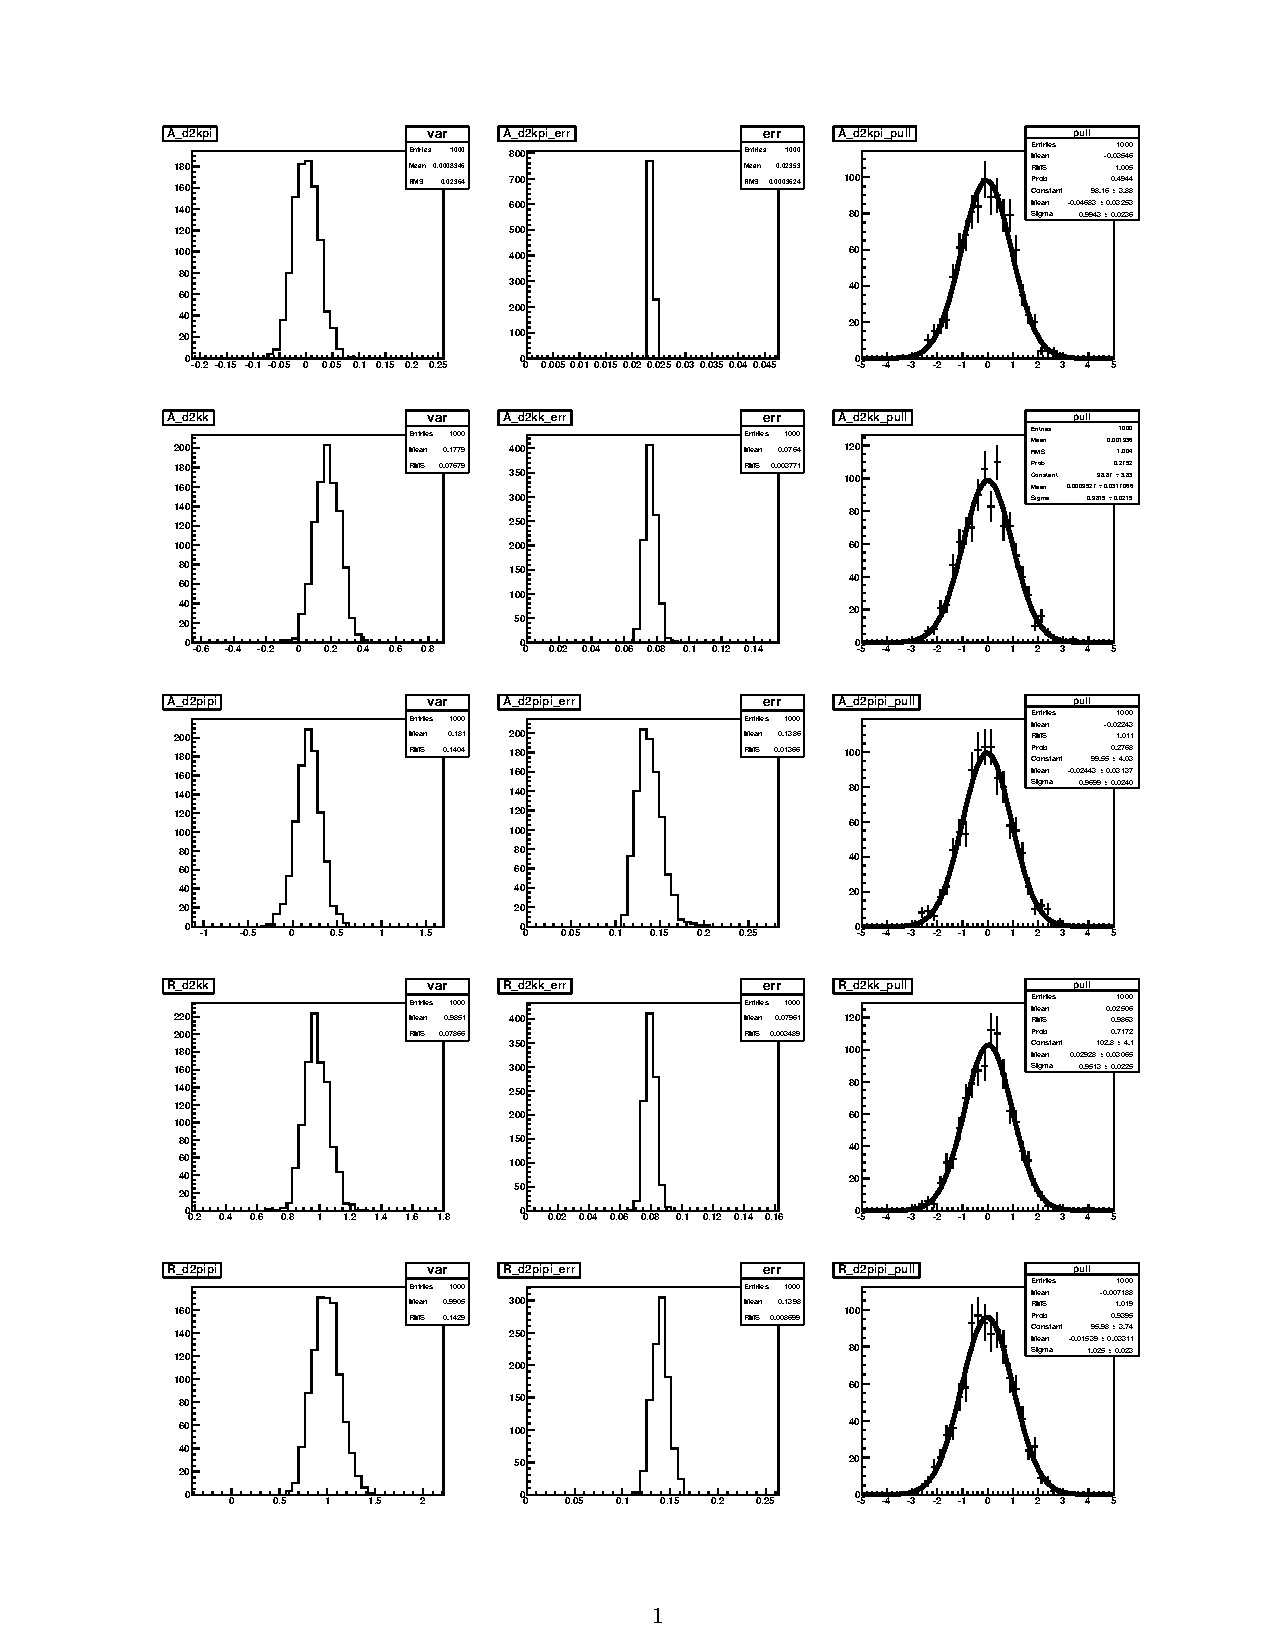
\includegraphics[page=1,trim = 0mm 24mm 0mm 15mm,clip,width=0.85\linewidth]{figures/results/toys.pdf}
\includegraphics[page=2,trim = 0mm 165mm 0mm 15mm,clip,width=0.85\linewidth]{figures/results/toys.pdf}
\caption{Results from pseudoexperiments for the two-body \CP observables in the fit. The left-hand column shows the fitted parameter distribution, the middle column shows the fit error distribution and the right-hand column are the pull distributions fitted with a Gaussian.}
\label{pulls1}
\end{figure}

\begin{figure}[!h]
\centering
\includegraphics[page=2,trim = 0mm 24mm 0mm 113mm,clip,width=0.85\linewidth]{figures/results/toys.pdf}
\includegraphics[page=3,trim = 0mm 165mm 0mm 15mm,clip,width=0.85\linewidth]{figures/results/toys.pdf}
\caption{Results from pseudoexperiments for the four-body \CP observables in the fit. The left-hand column shows the fitted parameter distribution, the middle column shows the fit error distribution and the right-hand column are the pull distributions fitted with a Gaussian.}
\label{pulls2}
\end{figure}

\subsection{Optimisation of BDT and \Kstar selection}
\label{sec:cpfit:optimisation}

To select \btodkst events, a BDT is implemented and selection requirements are applied to the \Kstar mass and \KS helicity angle to preferentially select events that proceed via a \Kstar meson, as described in Section \ref{sec:selection}. The BDT selection, \Kstar mass and \KS helicity angle selection requirements are optimised simultaneously with the aim of minimising the uncertainty on the \CP parameters, \Akpi, \Akk, \Apipi, \Rkk, \Rpipi, \Rptwo, \Rmtwo, \Akpipipi, \Apipipipi, \Rpipipipi, \Rpfour and \Rmfour. 

In order to perform this optimisation procedure, the selection is applied to data excluding any requirements on the \Kstarm mass or \KS helicity angle, and with only a loose BDT selection, requiring the BDT classifier to be greater than $-0.8$. With this setup, a single fit was performed to the two- and four-body favoured modes, similar to the fit in Section \ref{sec:massfit:fit}, to extract the expected signal, combinatoric and partially reconstructed yields. The signal and background efficiencies were calculated, from simulation and data respectively, for the various selections explored, namely:

\begin{itemize}
\item{The reconstructed \Kstarm mass lies within 50\mevcc, 75\mevcc, 100\mevcc of the known \Kstarm mass,}
\item{The magnitude of $\cos(\theta_{\KS})$ is greater than: 0, 0.1, 0.2, 0.3 and 0.4,}
\item{The BDT classifier is greater than: -0.8, -0.6, -0.4, -0.2, 0, 0.2, 0.4, 0.6, 0.7, 0.8, 0.9, 0.95.}
\end{itemize}

Using the yields extracted from the loose selection scenario described as well as the signal and background efficiencies, the estimated yields for the various selections are calculated. Data samples were generated based on the expected yields and efficiencies. The signal yield in the favoured \kpi and \kpipipi modes are estimated from the fit to data, and the the yield ratios and asymmetries, used to extract the yields in the other \Dz decay modes, were inferred from the physics parameters, $r_B$, $\delta_B$ and \Pgamma, using Equations \ref{exp_Acp} - \ref{exp_R4pi}. For this optimisation procedure values of $r_B = 0.1$, $\delta_B = 150^{\circ}$ and $\gamma = 70^{\circ}$ were assumed. The value for \Pgamma is taken from the central value of the current \lhcb combination and $r_B$ is assumed to be the same as the equivalent ratio for \decay{\Bm}{\D\Km} decays. Although the value of $\delta_B$ is completely unknown, the optimisation was repeated for various values of $\delta_B$ and it was found that the choice of selection is not sensitive to $\delta_B$.

Pseudoexperiments, as described in Section \ref{sec:cpfit:fitterbias}, are performed for different selections to calculate the fit uncertainty for each selection. The fit uncertainty is taken to be the mean of the uncertainty distribution. For optimising the selection for the GLW modes, the fit uncertainty was minimised for \Akk, \Rkk, \Apipi and \Rpipi. For example, Figure \ref{optimisation} shows the fit uncertainty in \Rkk as a function of the \KS helicity angle selection point, for different \Kstar mass requirements. In this figure, the minimum uncertainty is achieved by requiring the reconstructed \Kstar mass to lie within 75\mevcc of the known \Kstar mass and magnitude if the \KS helicity angle greater than 0.3. This describes the \Kstar requirements chosen for the final selection after investigating uncertainties in other variables. Similarly, the requirement on the BDT classifier is chosen to be greater than 0.6 for LL candidates and 0.7 for DD candidates. The BDT selection for the ADS modes was optimised to minimise the fit errors in \Rptwo and \Rmtwo. Studies were performed to investigate a tighter BDT selection for the ADS mode as illustrated in Figure \ref{adsoptimisation}, showing that the uncertainty in \Rptwo continues to decrease as the BDT requirement is tightened. The tighter BDT cut in the ADS mode for DD candidates was chosen as it resulted in a lower uncertainty on \Rptwo and \Rmtwo due to a reduction in the background rejection from 7\% to 2\% while retaining 80\% of the signal. 

\begin{figure}
\centering
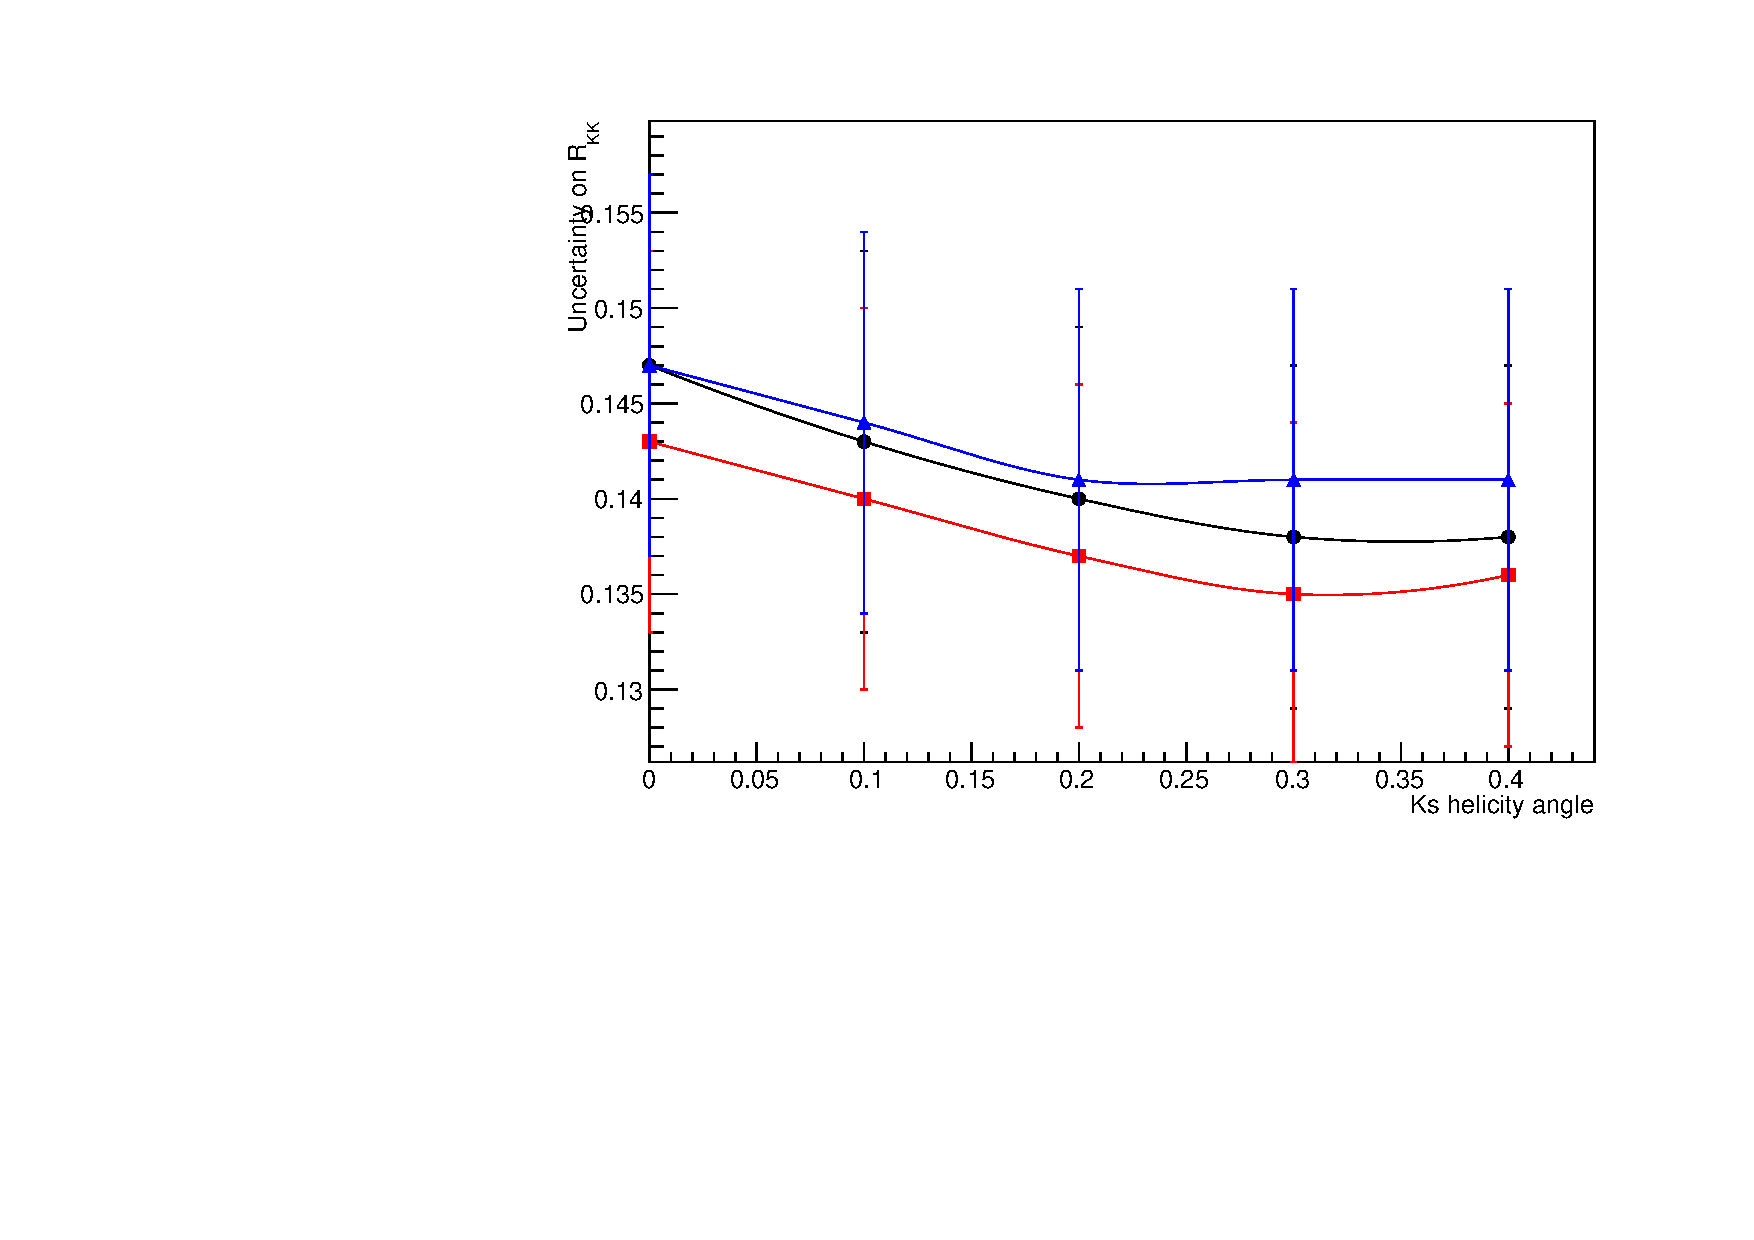
\includegraphics[width=0.8\linewidth]{figures/selection/optimisation.pdf}
\caption{Value of the uncertainty on \Rkk as a function of \KS helicity angle selection for different \Kstar mass selections. The black curve is using a \Kstar mass window of 100 MeV, the red curve is using a \Kstar mass window of 75 MeV and the blue curve is using a \Kstar mass window of 50 MeV. The minimum uncertainty is given for a \Kstar mass window of 75 MeV and \KS helicity angle of 0.3. This was the final \Kstar selection chosen after investigating uncertainties in other variables.}
\label{optimisation}
\end{figure}

\begin{figure}
\centering
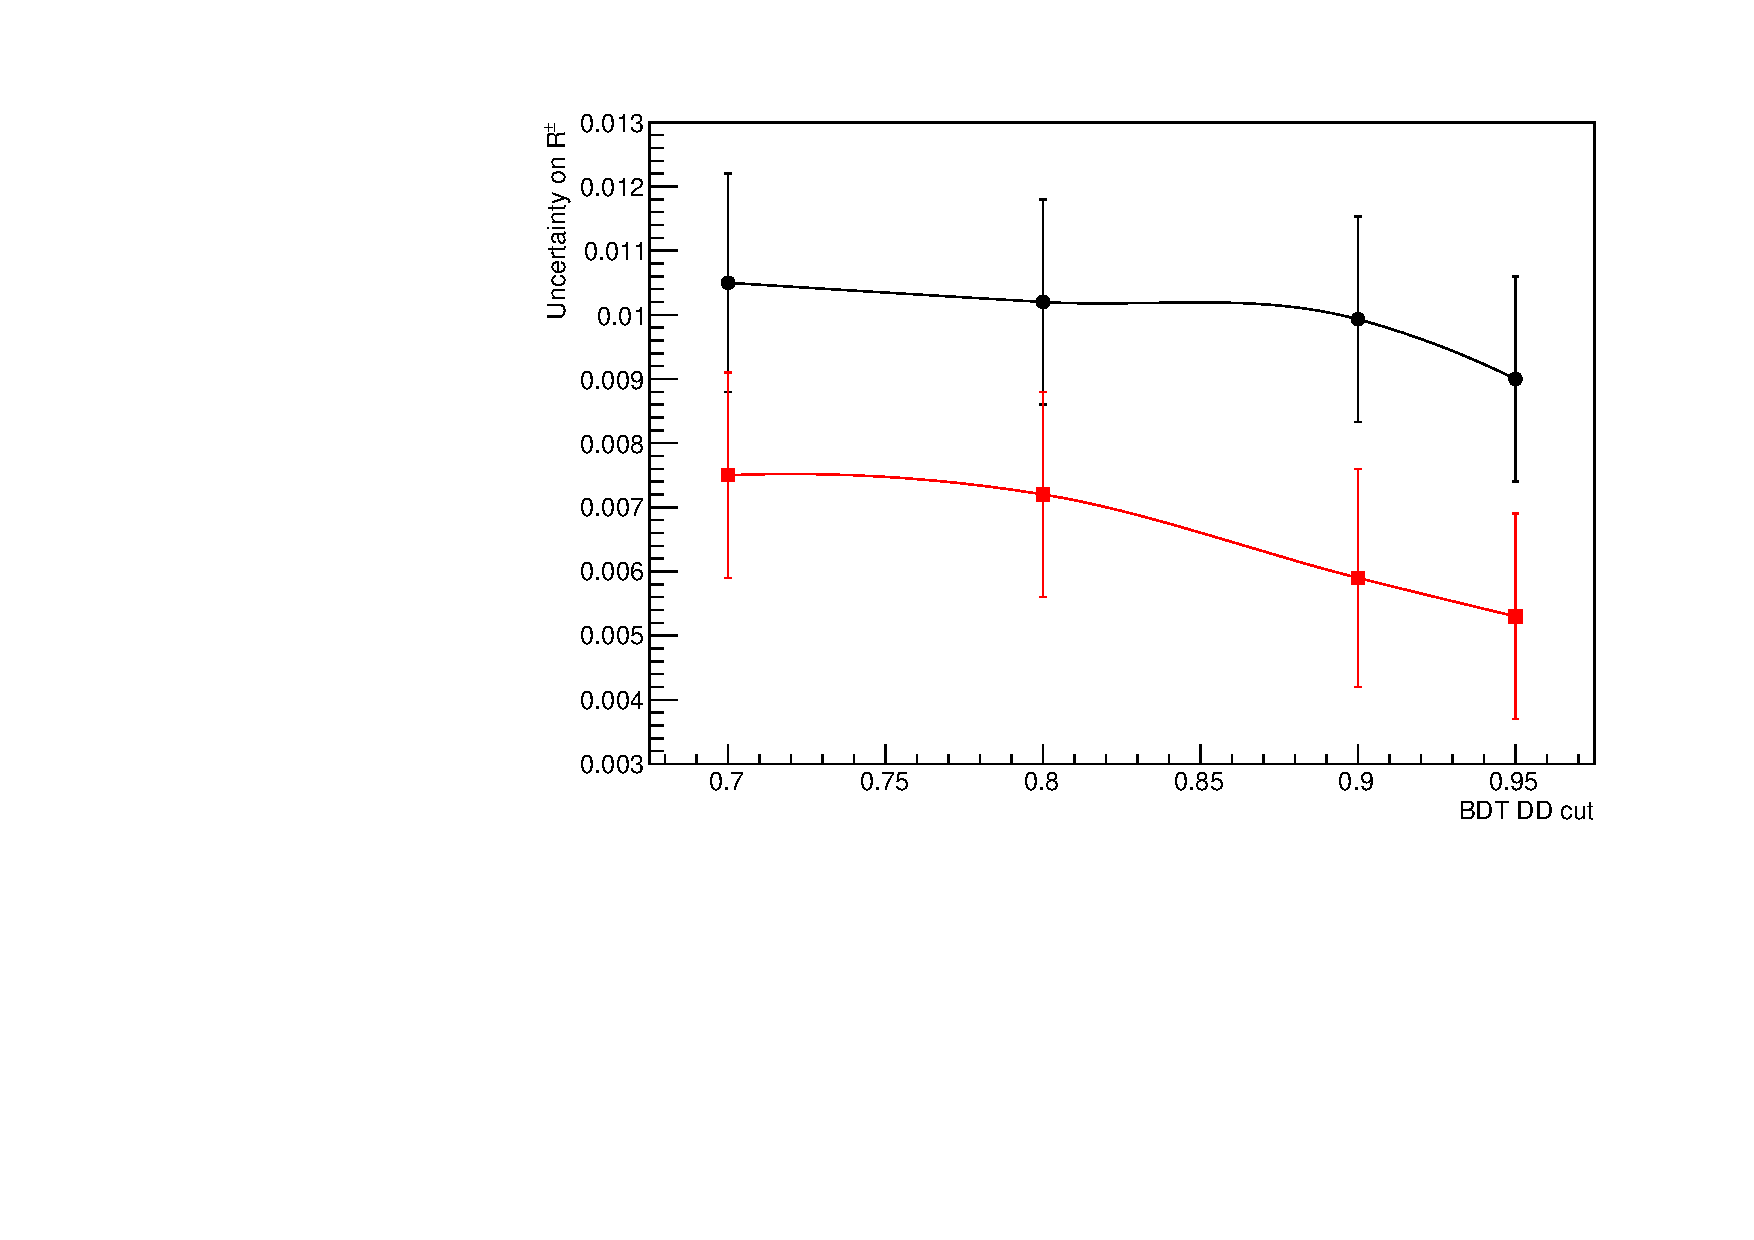
\includegraphics[width=0.8\linewidth]{figures/selection/ADSoptimisation.pdf}
\caption{Value of the uncertainty on \Rptwo and \Rmtwo as a function of BDT\_DD cut in the ADS mode. These toys were run with a BDT LL cut of 0.6 on all modes and BDT DD cut of 0.7 on all modes other than the ADS. The black curve is the uncertainty of \Rptwo and the red curve is the uncertainty of \Rmtwo. Although the uncertainty continues to decrease for a BDT cut of 0.95, this resulted in a significant drop in signal efficiency, therefore a cut of 0.9 was chosen for the ADS.}
\label{adsoptimisation}
\end{figure}

In cases when the figure of merits in these optimisation studies are not especially sensitive to changes in the selection, the selection giving the highest coherence, i.e. tighter \Kstarm selection, is chosen. For the BDT selection the signal and background efficiencies are also taken into account. The final selection chosen is:

\begin{itemize}
\item{The reconstructed \Kstarm mass must lie within 75\mev of the known \Kstarm mass.}
\item{The magnitude of $\cos(\theta_{\KS})$ is required to be greater than 0.3}
\item{The BDT classifier is required to be greater than 0.6 for LL candidates and greater than 0.7 for DD candidates, except in the ADS mode where it is required to be greater than 0.6 for LL candidates and 0.9 for DD candidates.}
\end{itemize}

A significantly lower combinatoric rate is observed in the ADS modes compared to the corresponding favoured \kpi and \kpipipi modes. The choice of BDT selection for the ADS modes is found to remain optimal when tested against a scenario of the observed low combinatoric in the ADS mode. 

%%%%%%%%%%%%%%%%%%%%%%%%
\section{Fit results}
\label{sec:cpfit:results}

The \CP fit, setup as described in Section \ref{sec:cpfit:setup}, is performed on data. The mass projection is each of the bins of the \CP fit, when performed on data, are shown in Figures \ref{datafit2bodyRun1}, \ref{datafit4bodyRun1}, \ref{datafit2bodyRun2} and \ref{datafit4bodyRun2}. Table \ref{cpfitresultsphysics} shows the \CP fit results of the \CP observables of interest and Table \ref{cpfitresultsshapes} shows the fit results for the favoured \kpi and \kpipipi signal yields and the shape parameters. All the combinatoric yields are left to vary in the \CP fit and these results are shown in Table \ref{cpfitresultscomb}. The fitted yields obtained for running the fit with \Bp and \Bm samples combined are given in Table \ref{fittedyields}. 

\begin{sidewaysfigure}[h]
\centering
\subfloat[$K\pi$, LL]{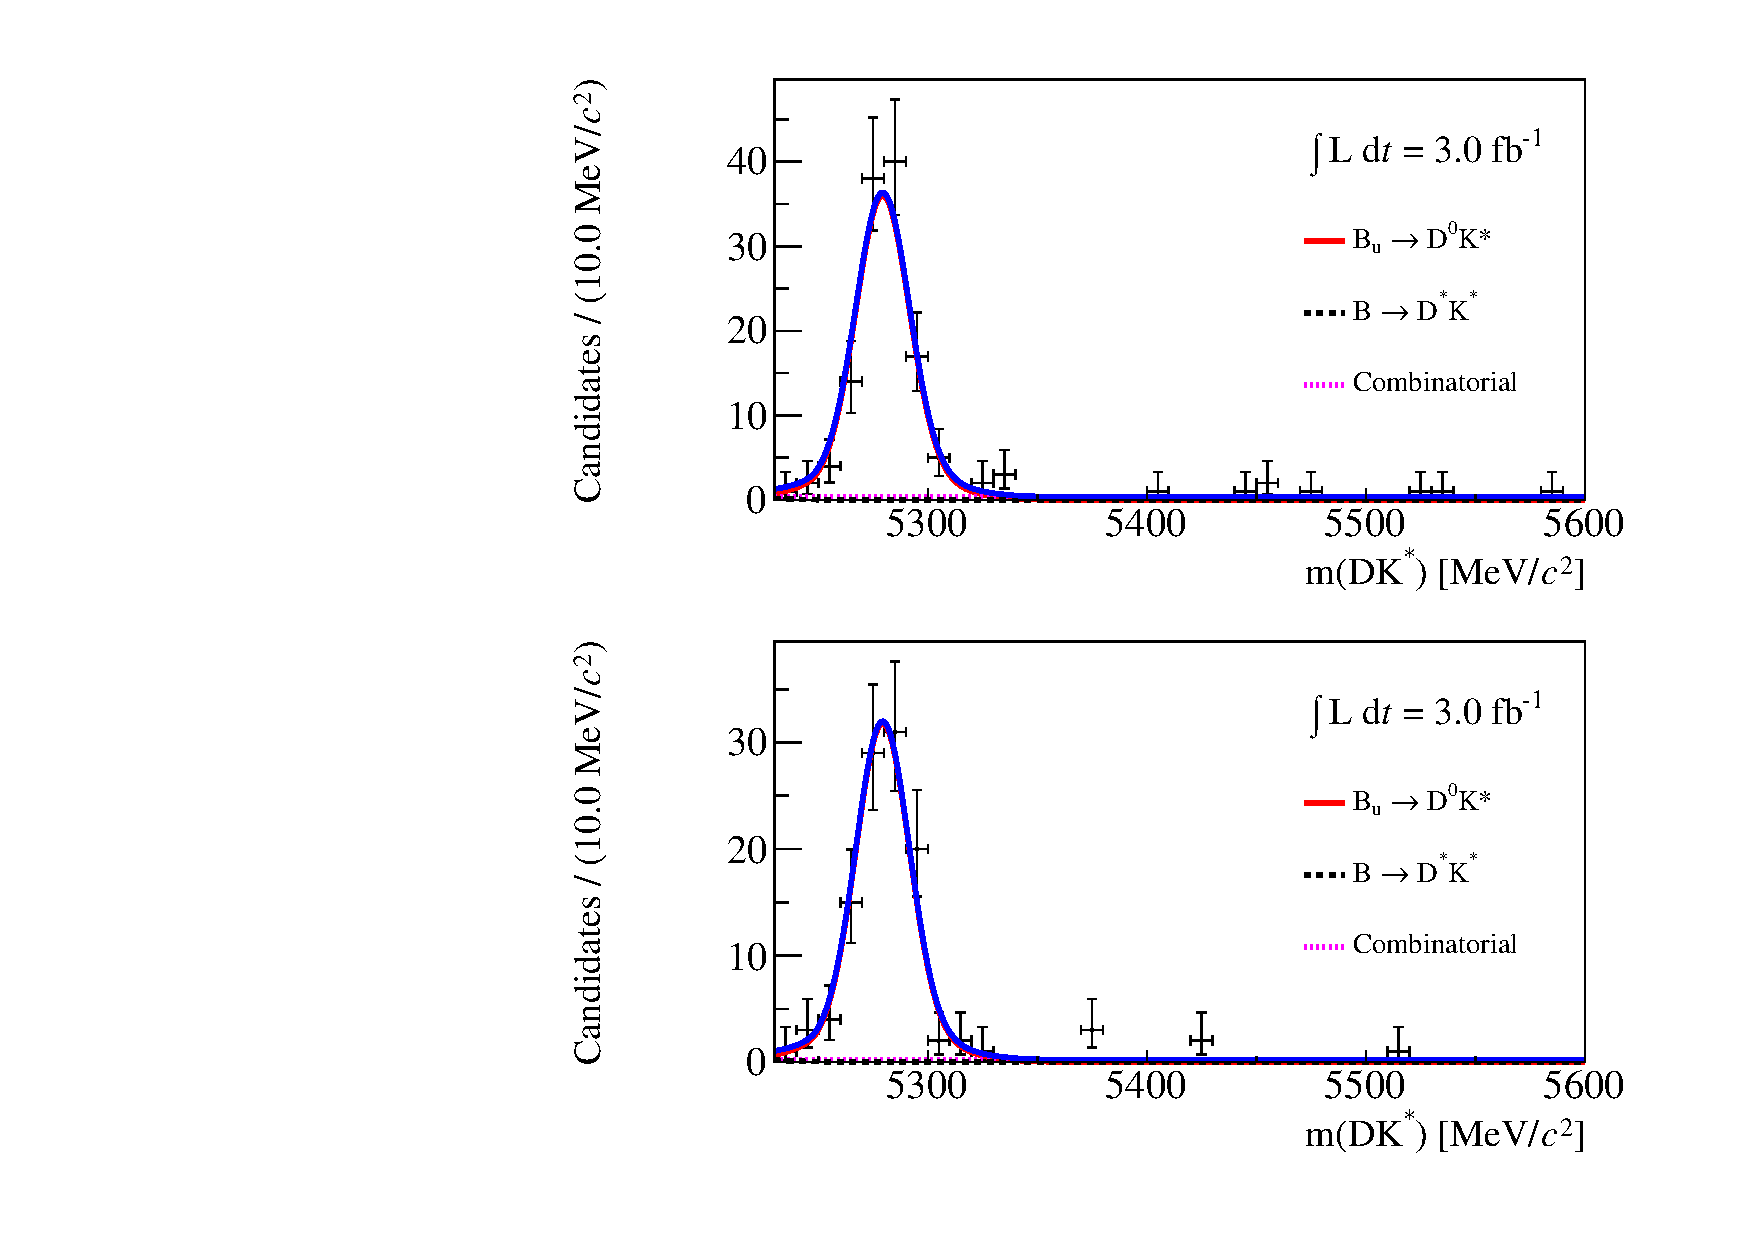
\includegraphics[width=0.25\linewidth]{figures/results/canvas_d2kpi_LL_run1.pdf}}
\hfill
\subfloat[$KK$, LL]{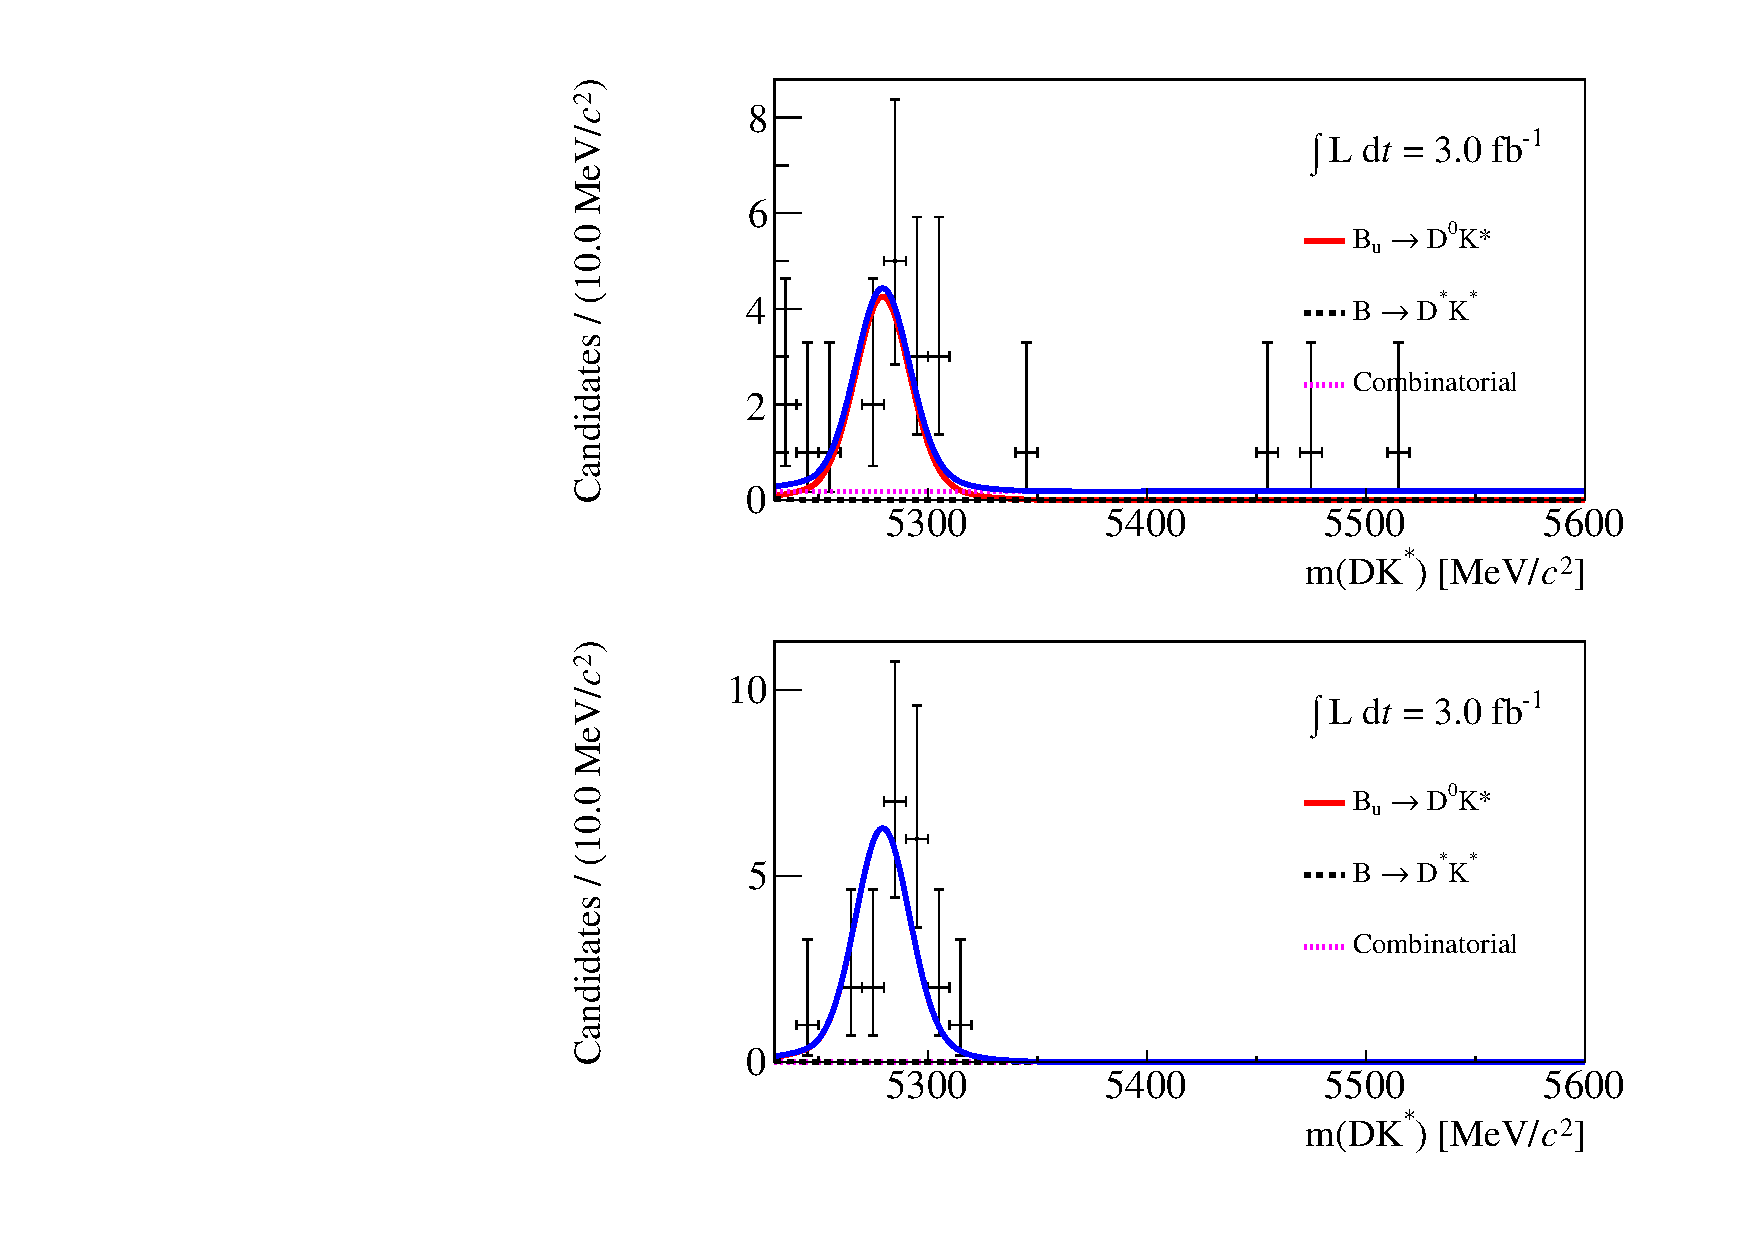
\includegraphics[width=0.25\linewidth]{figures/results/canvas_d2kk_LL_run1.pdf}}
\hfill
\subfloat[$\pi\pi$, LL]{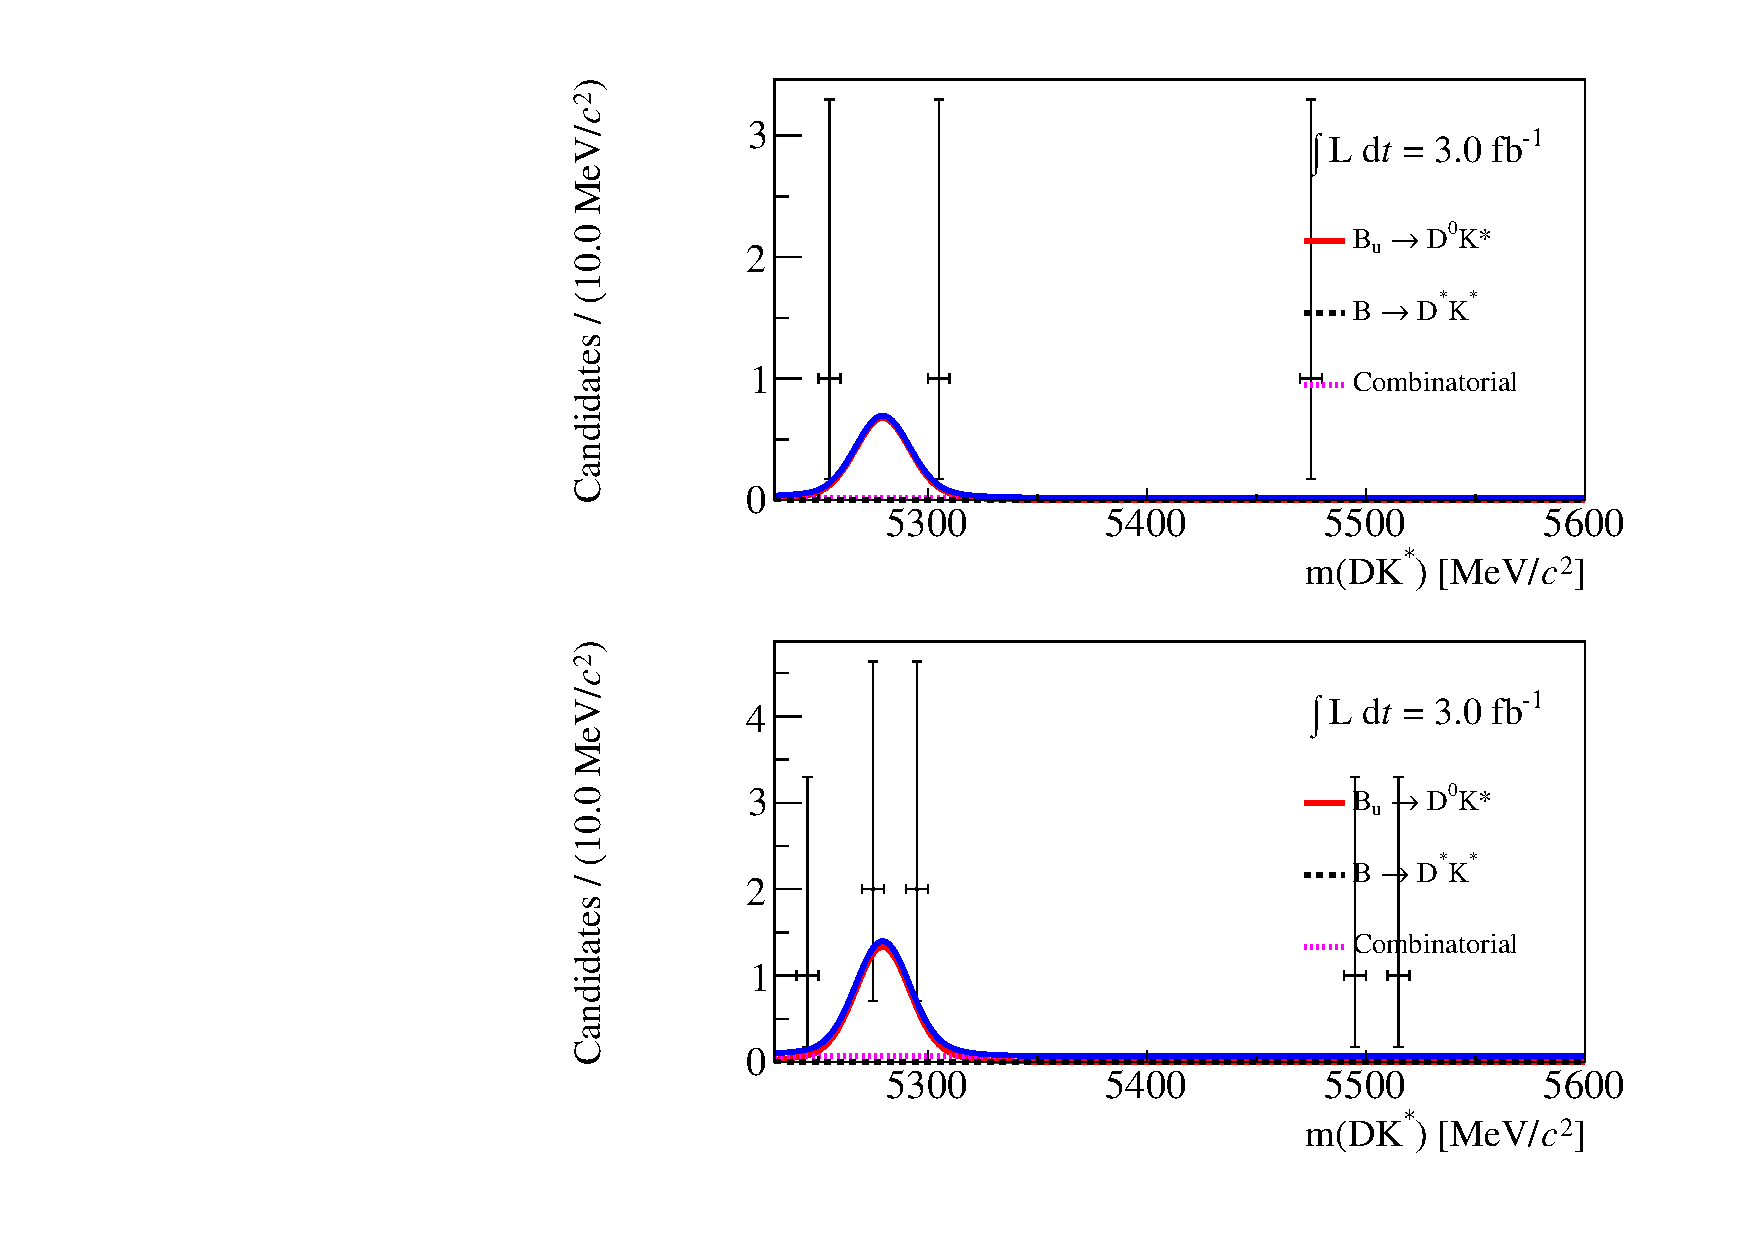
\includegraphics[width=0.25\linewidth]{figures/results/canvas_d2pipi_LL_run1.pdf}}
\hfill
\subfloat[$\pi K$, LL]{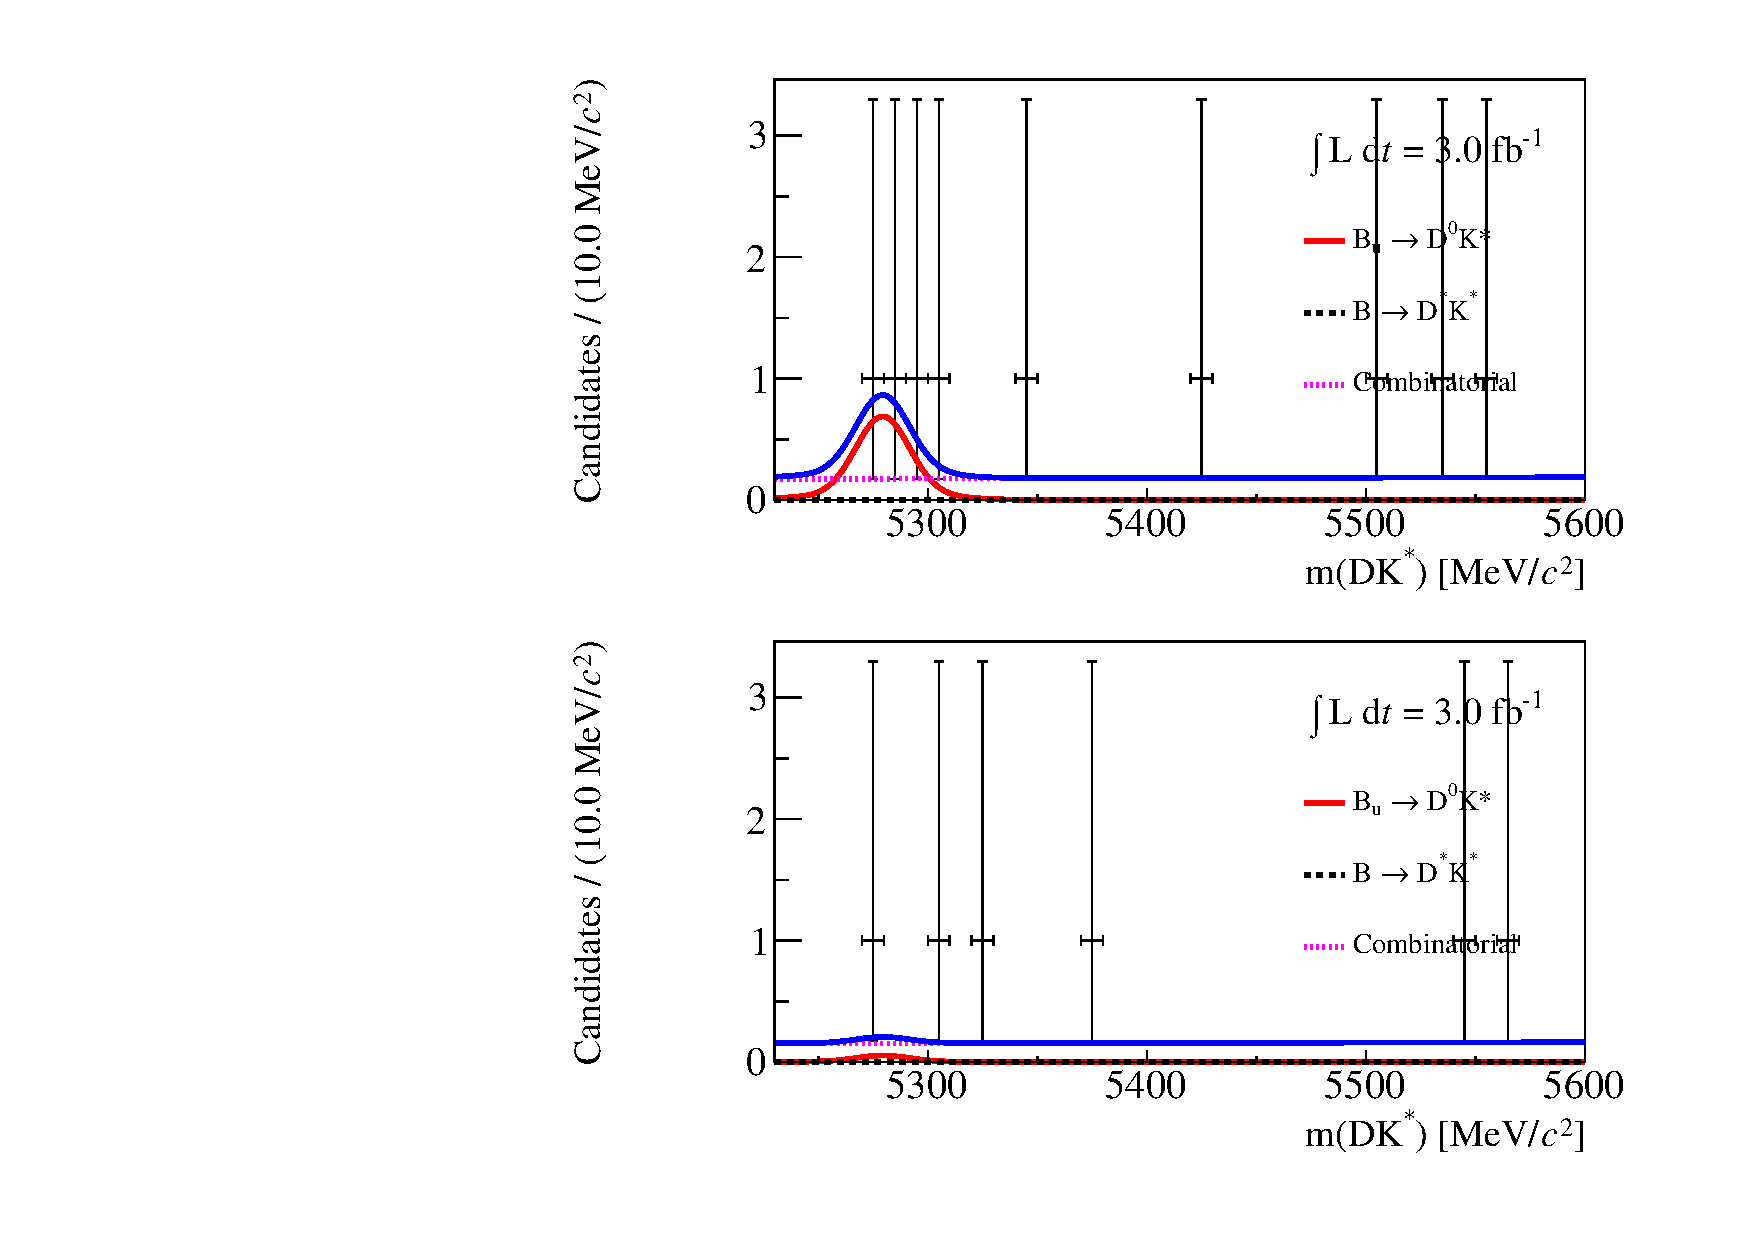
\includegraphics[width=0.25\linewidth]{figures/results/canvas_d2pik_LL_run1.pdf}}
\hfill
\subfloat[$K\pi$, DD]{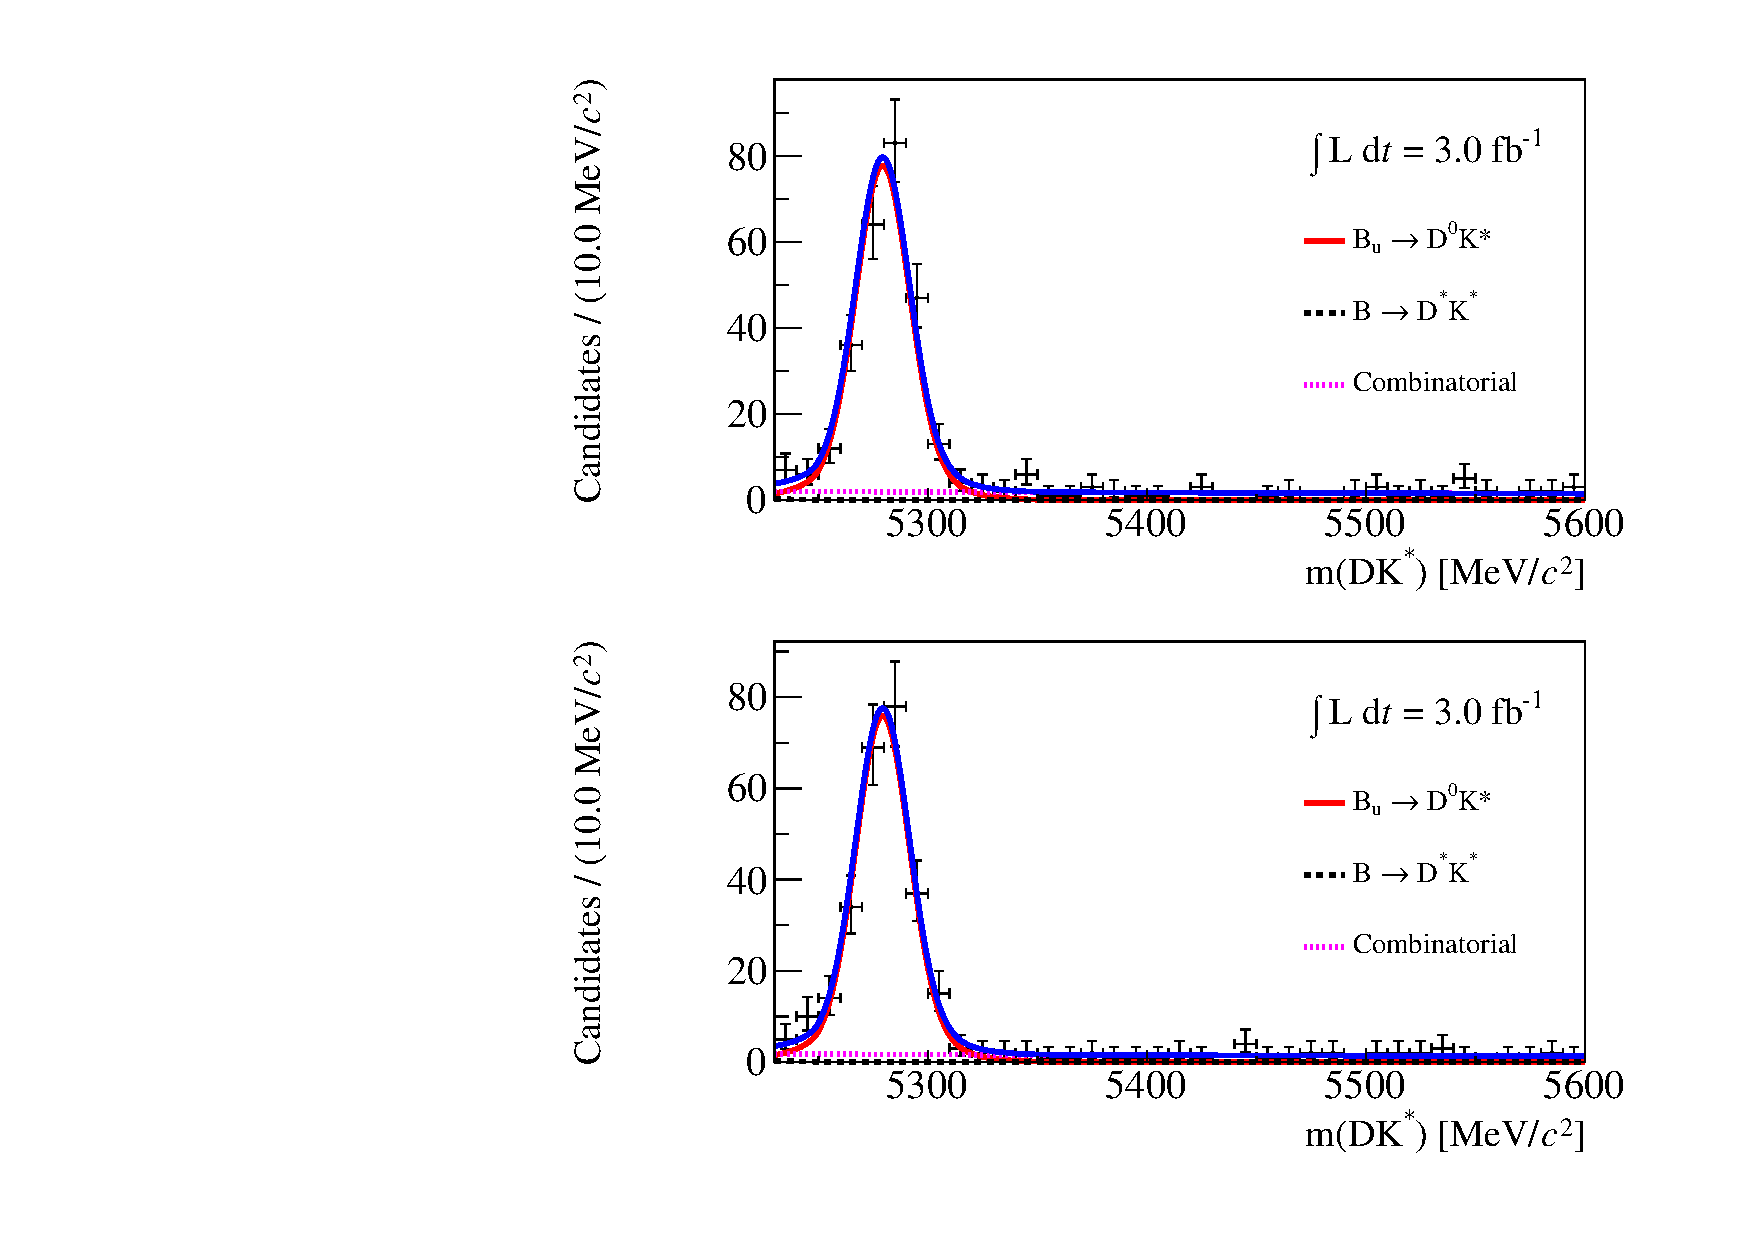
\includegraphics[width=0.25\linewidth]{figures/results/canvas_d2kpi_DD_run1.pdf}}
\hfill
\subfloat[$KK$, DD]{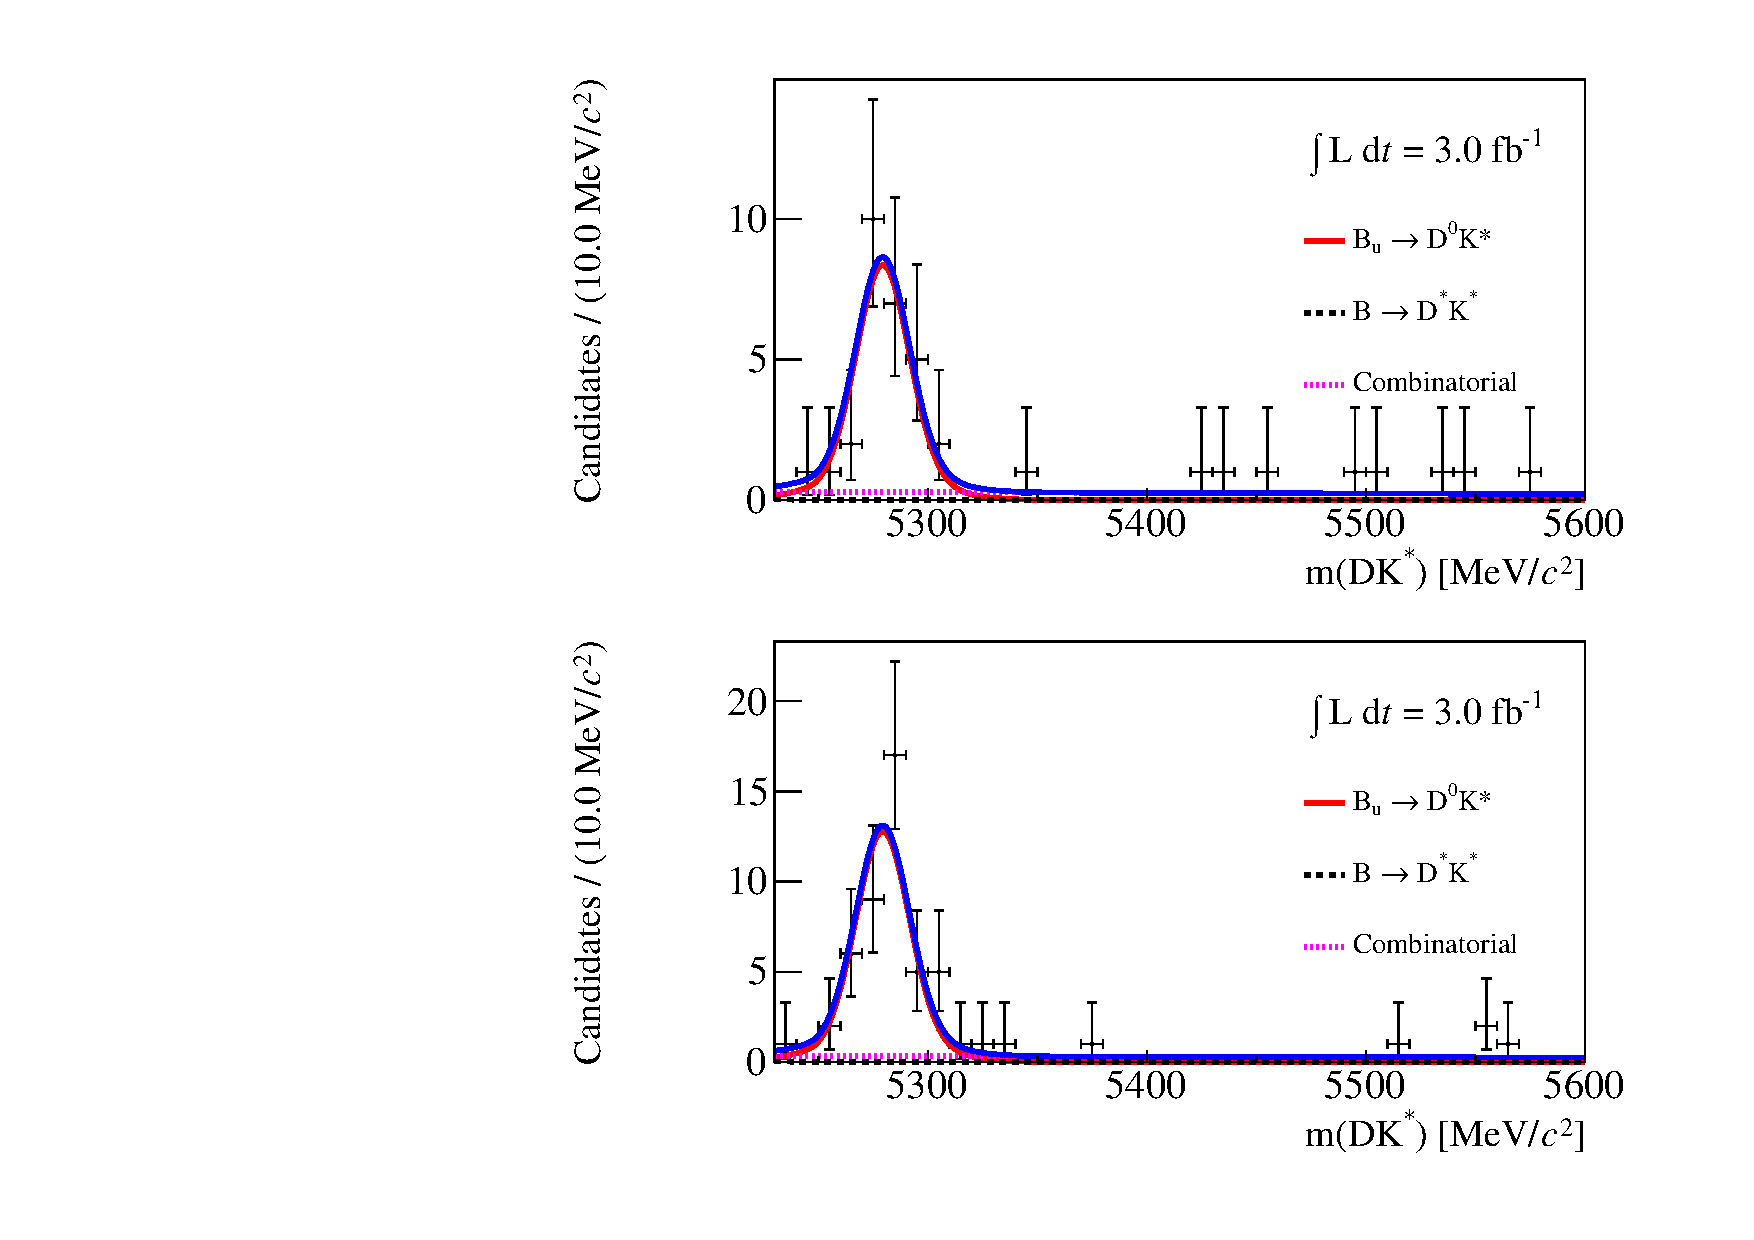
\includegraphics[width=0.25\linewidth]{figures/results/canvas_d2kk_DD_run1.pdf}}
\hfill
\subfloat[$\pi\pi$, DD]{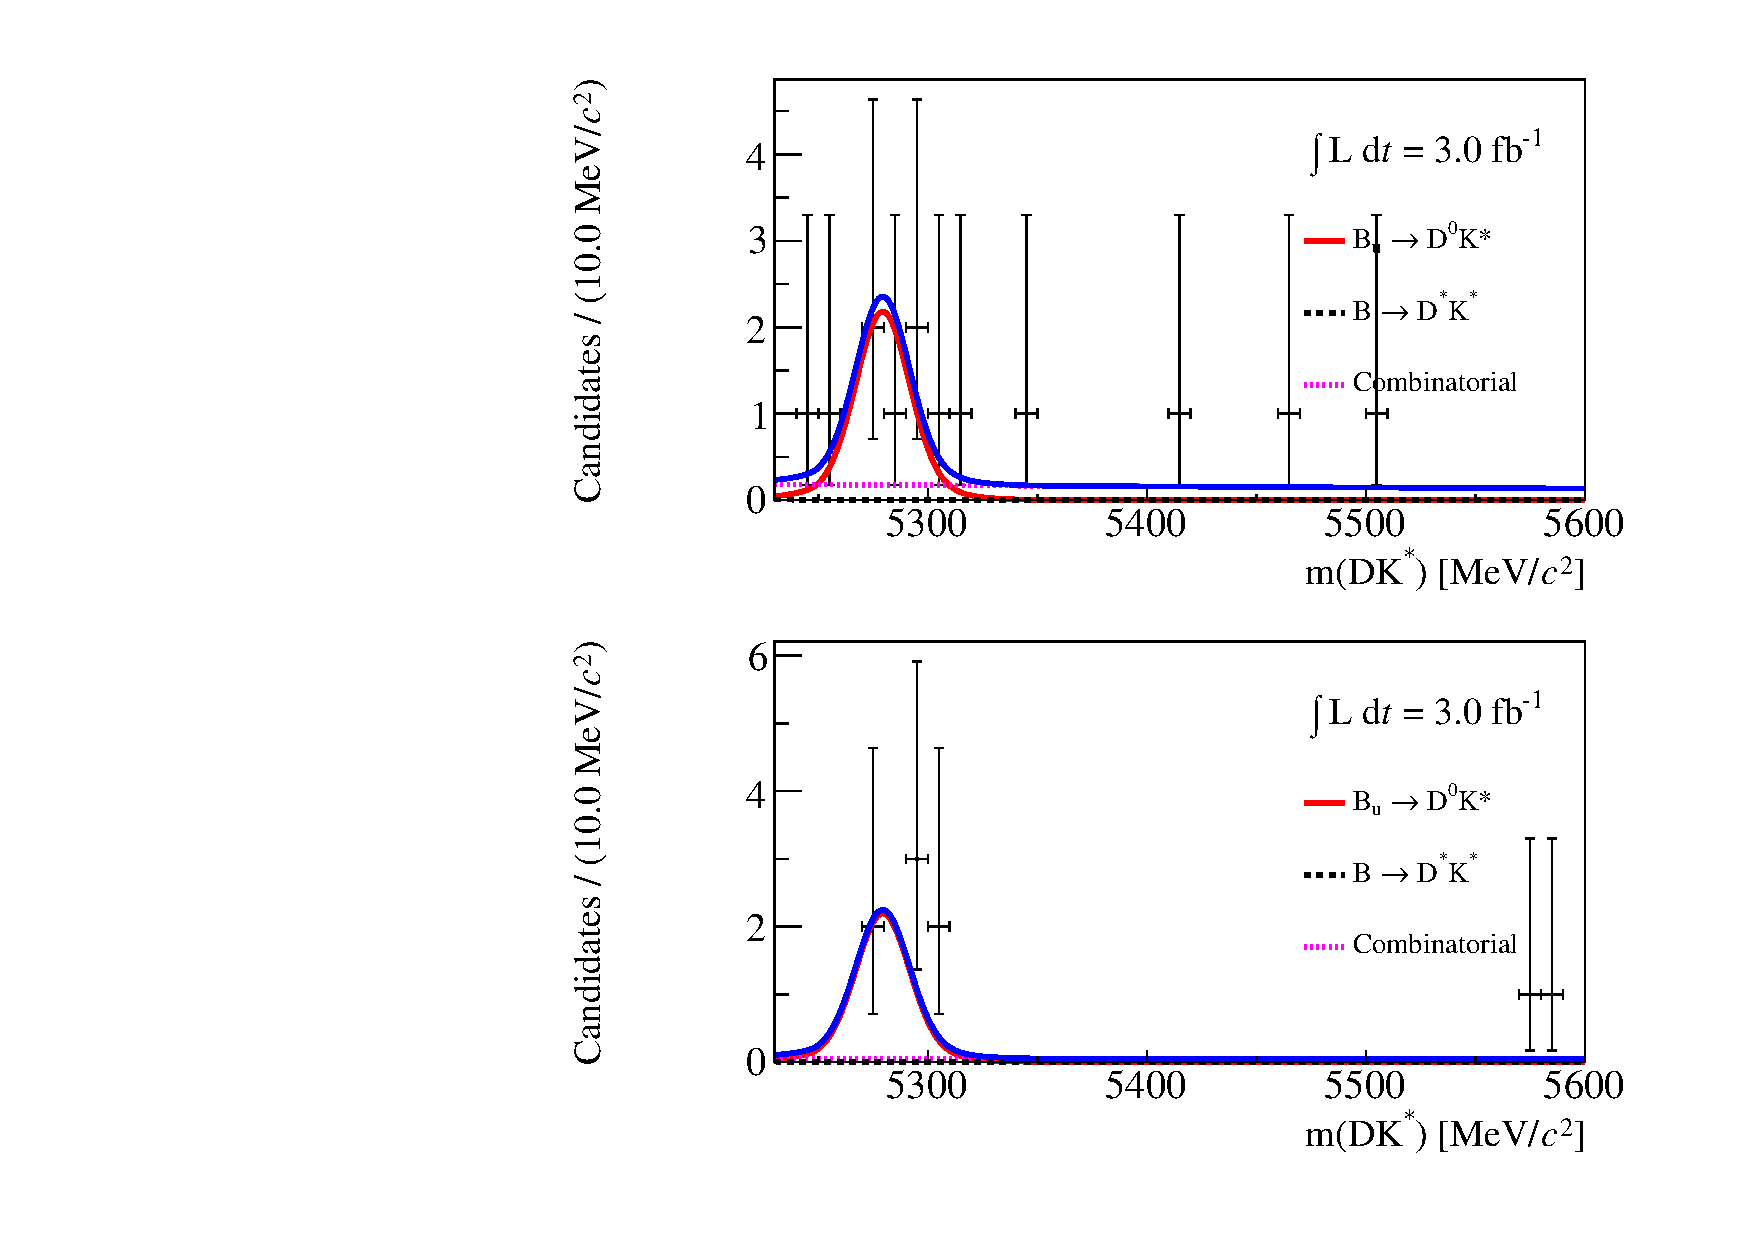
\includegraphics[width=0.25\linewidth]{figures/results/canvas_d2pipi_DD_run1.pdf}}
\hfill
\subfloat[$\pi K$, DD]{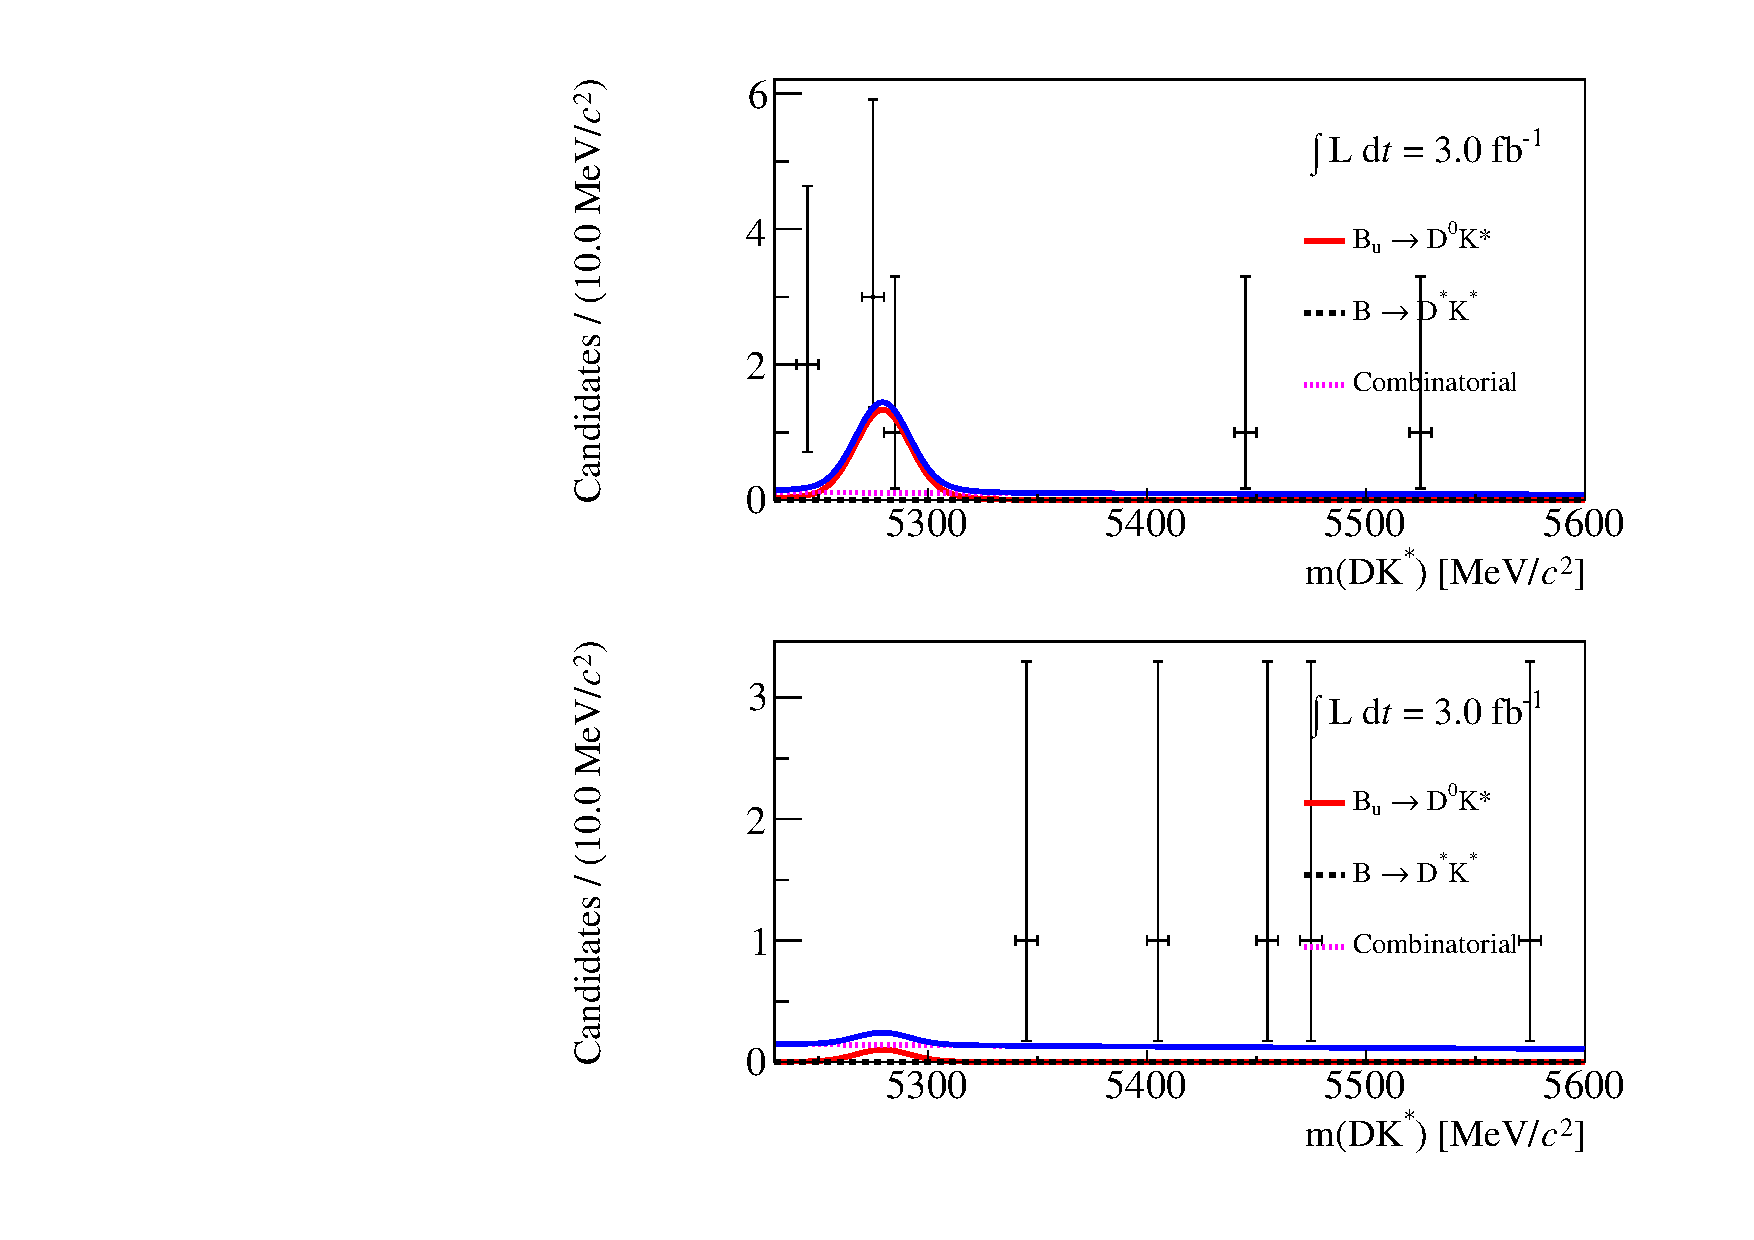
\includegraphics[width=0.25\linewidth]{figures/results/canvas_d2pik_DD_run1.pdf}}
\caption{Results of the simultaneous fit for \runone data for two-body modes. In each pair the top plot is for \Bp decays and the bottom plot is for \Bm decays.}
\label{datafit2bodyRun1}
\end{sidewaysfigure}

\begin{sidewaysfigure}[h]
\centering
\subfloat[$K\pi\pi\pi$, LL]{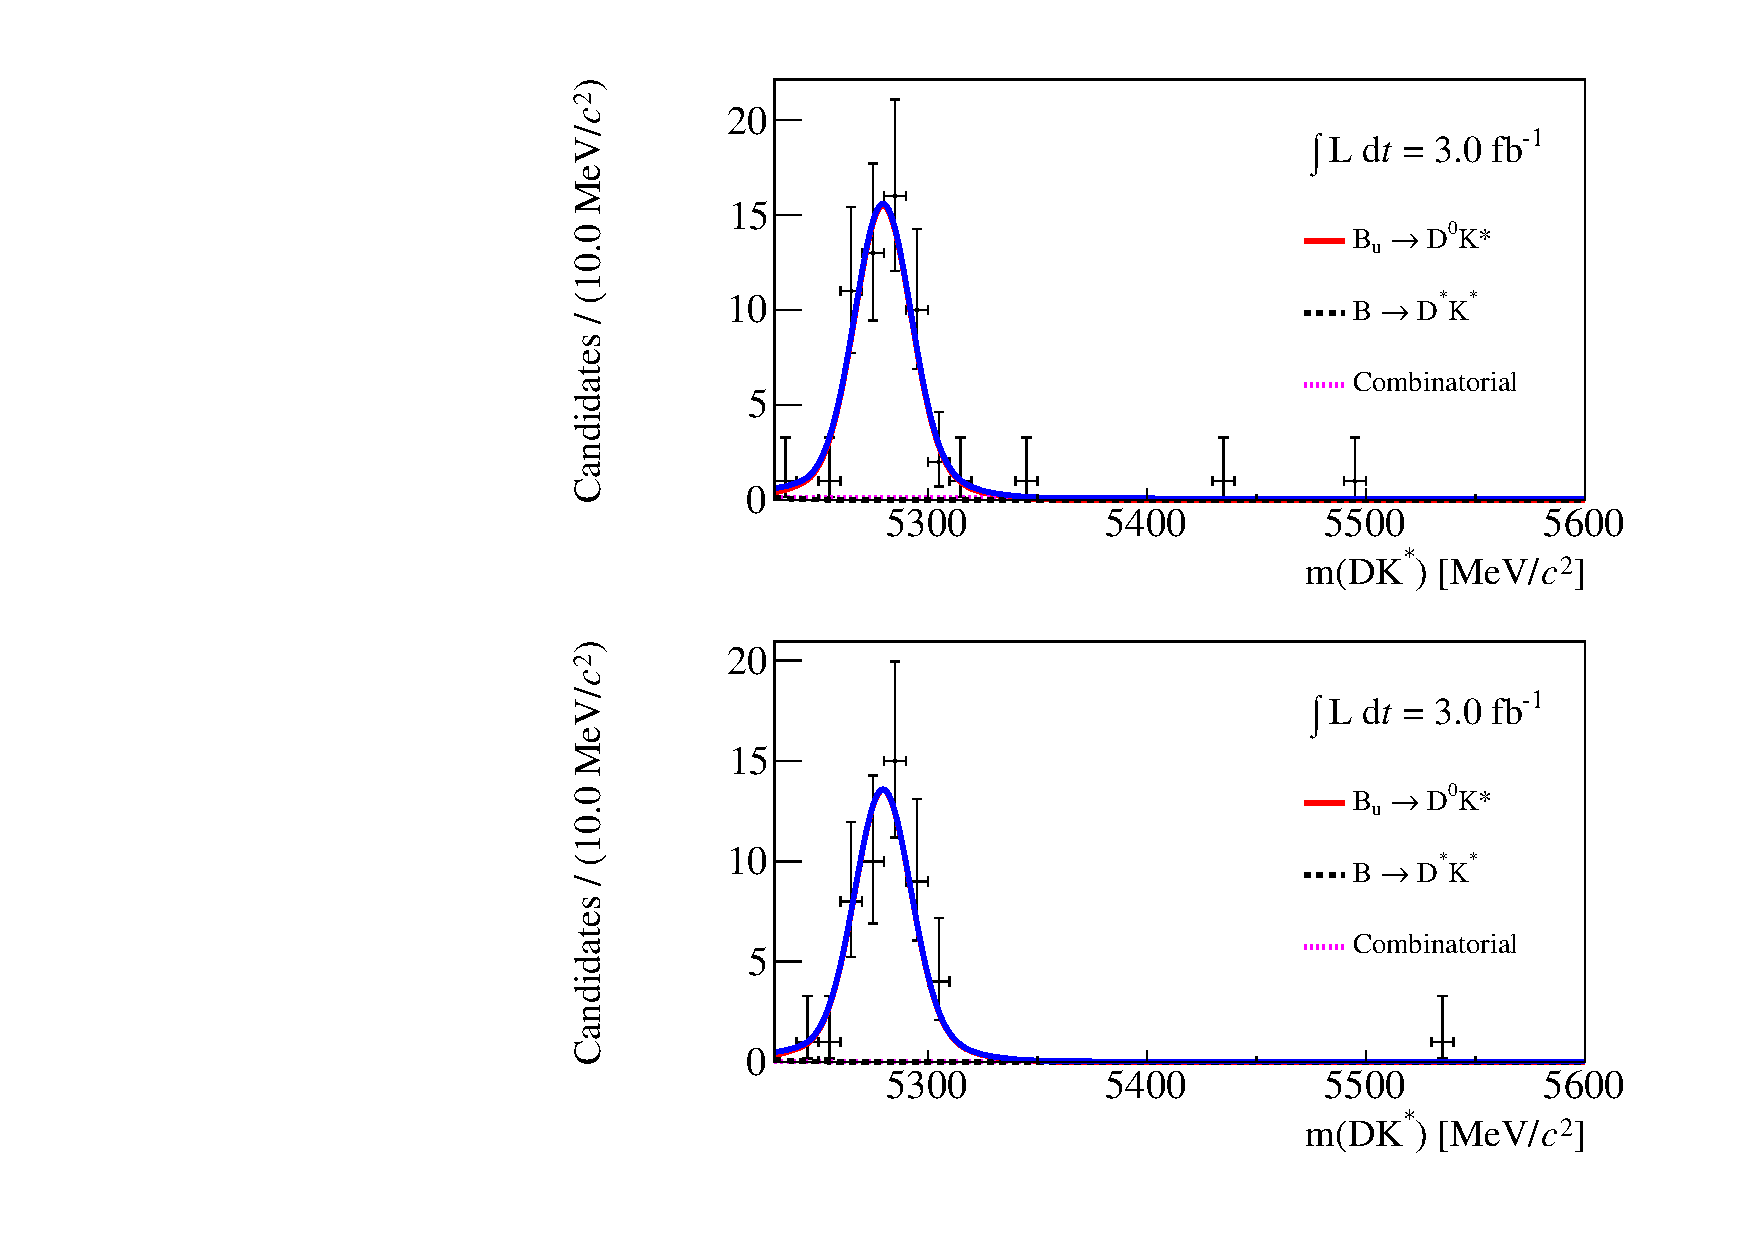
\includegraphics[width=0.3\linewidth]{figures/results/canvas_d2kpipipi_LL_run1.pdf}}
\hfill
\subfloat[$\pi\pi\pi\pi$, LL]{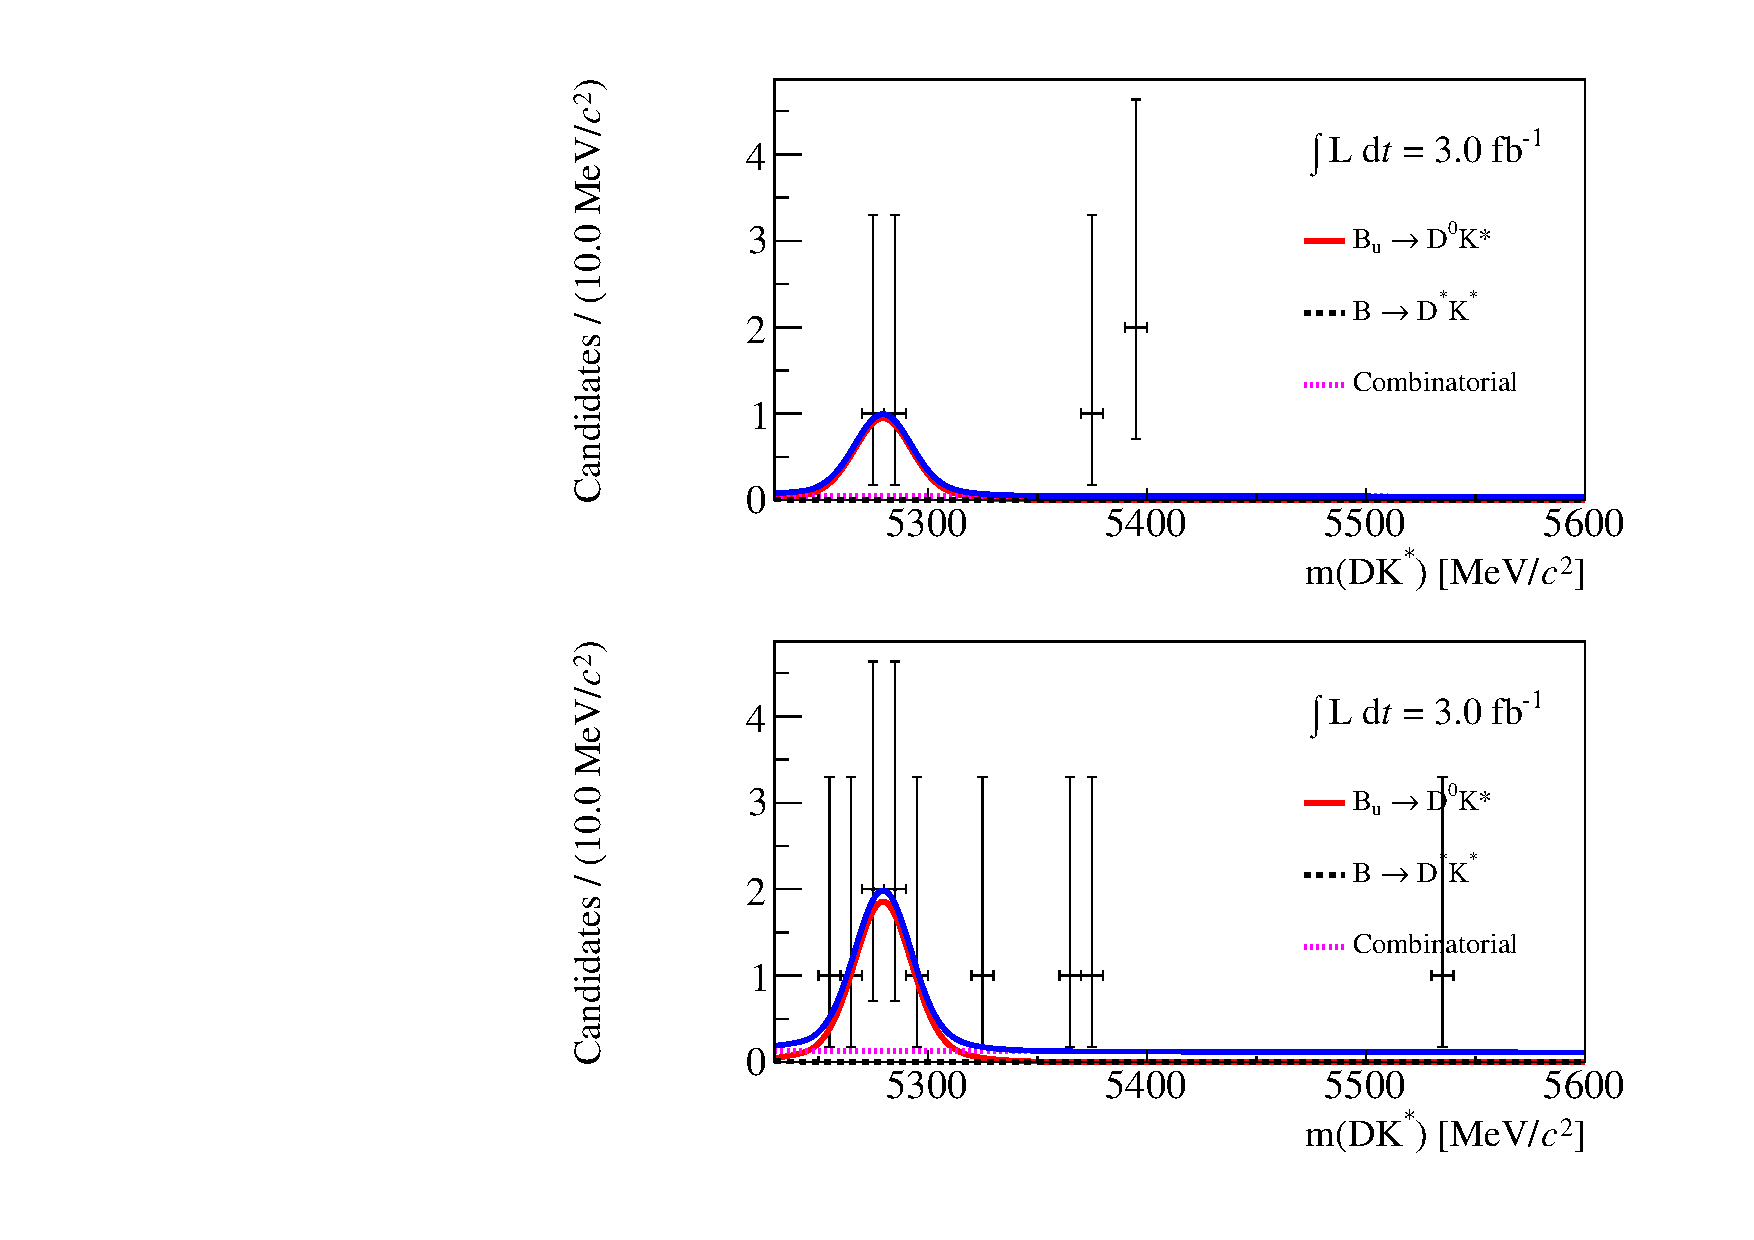
\includegraphics[width=0.3\linewidth]{figures/results/canvas_d2pipipipi_LL_run1.pdf}}
\hfill
\subfloat[$\pi K\pi\pi$, LL]{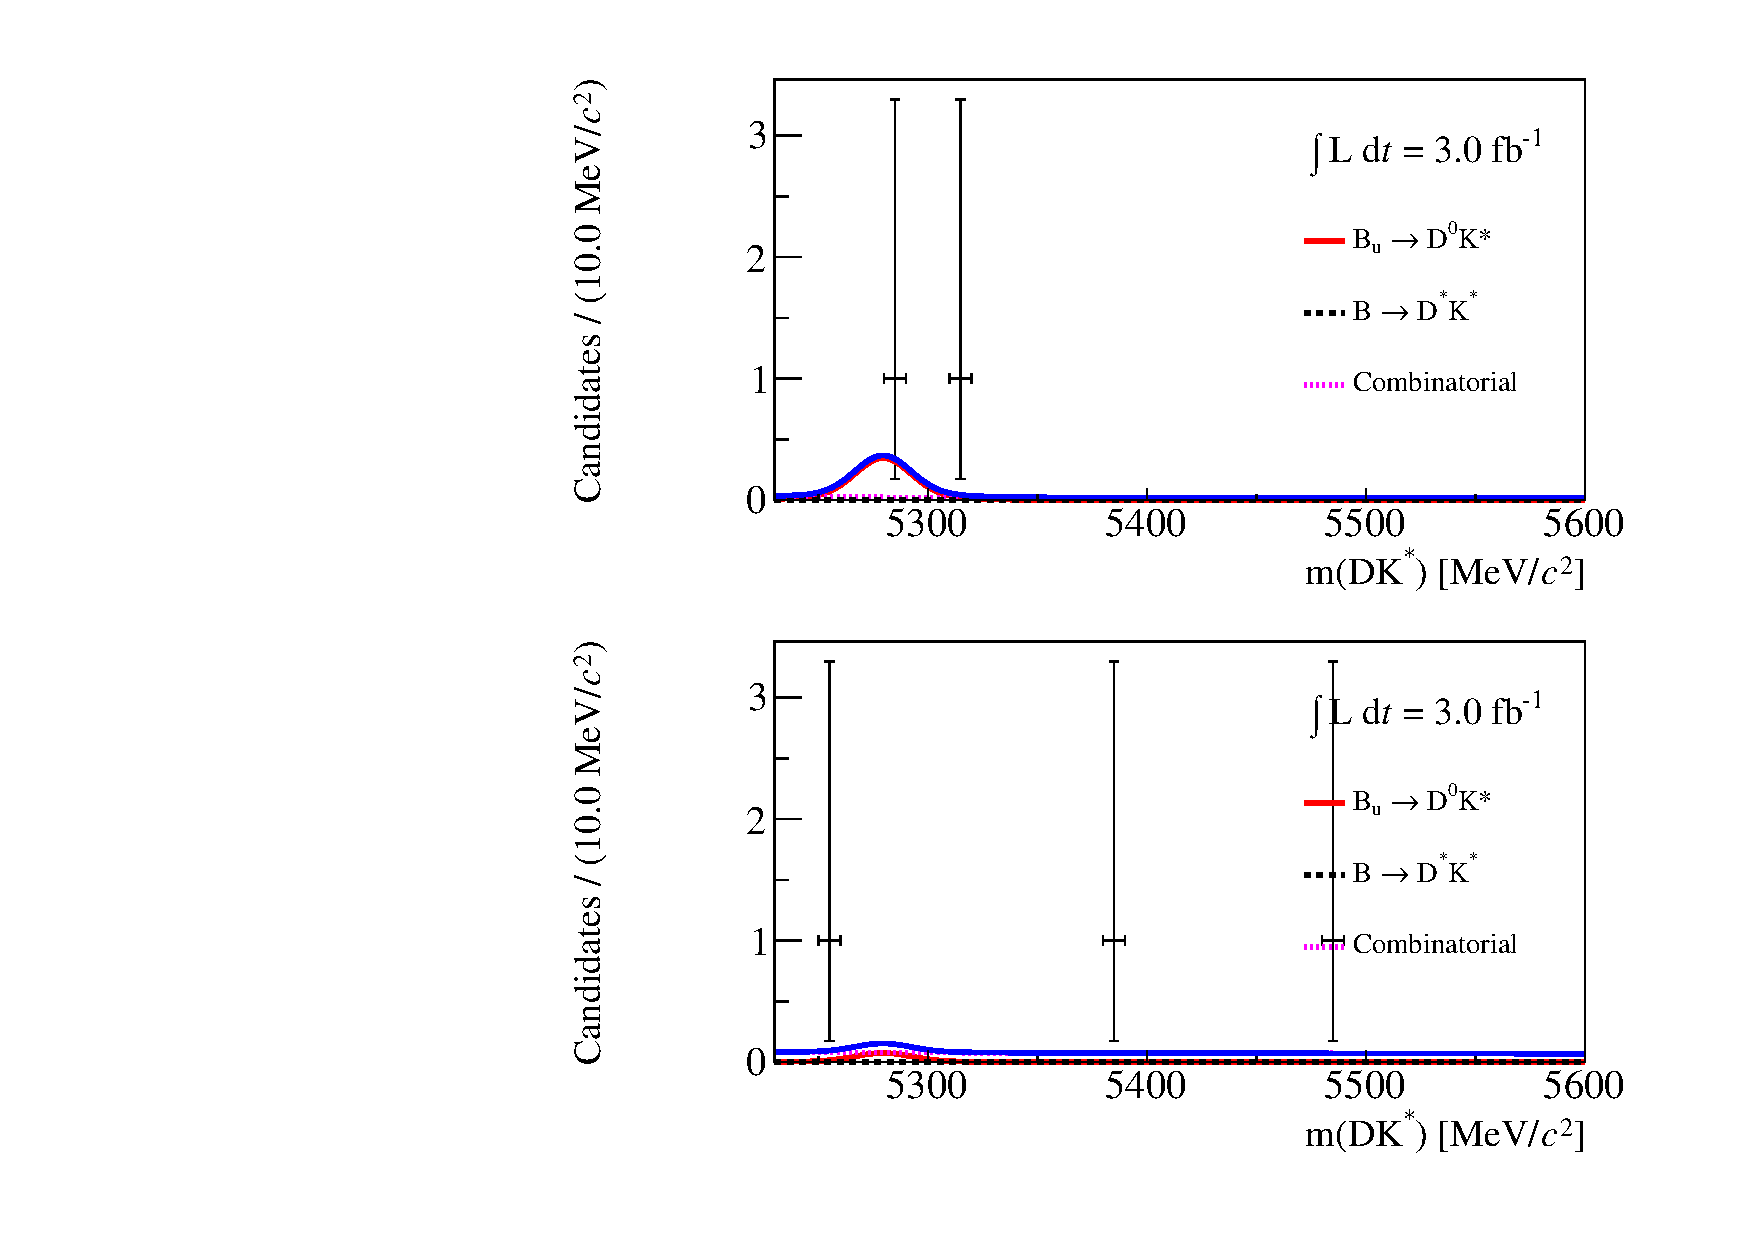
\includegraphics[width=0.3\linewidth]{figures/results/canvas_d2pikpipi_LL_run1.pdf}}
\hfill
\subfloat[$K\pi\pi\pi$, DD]{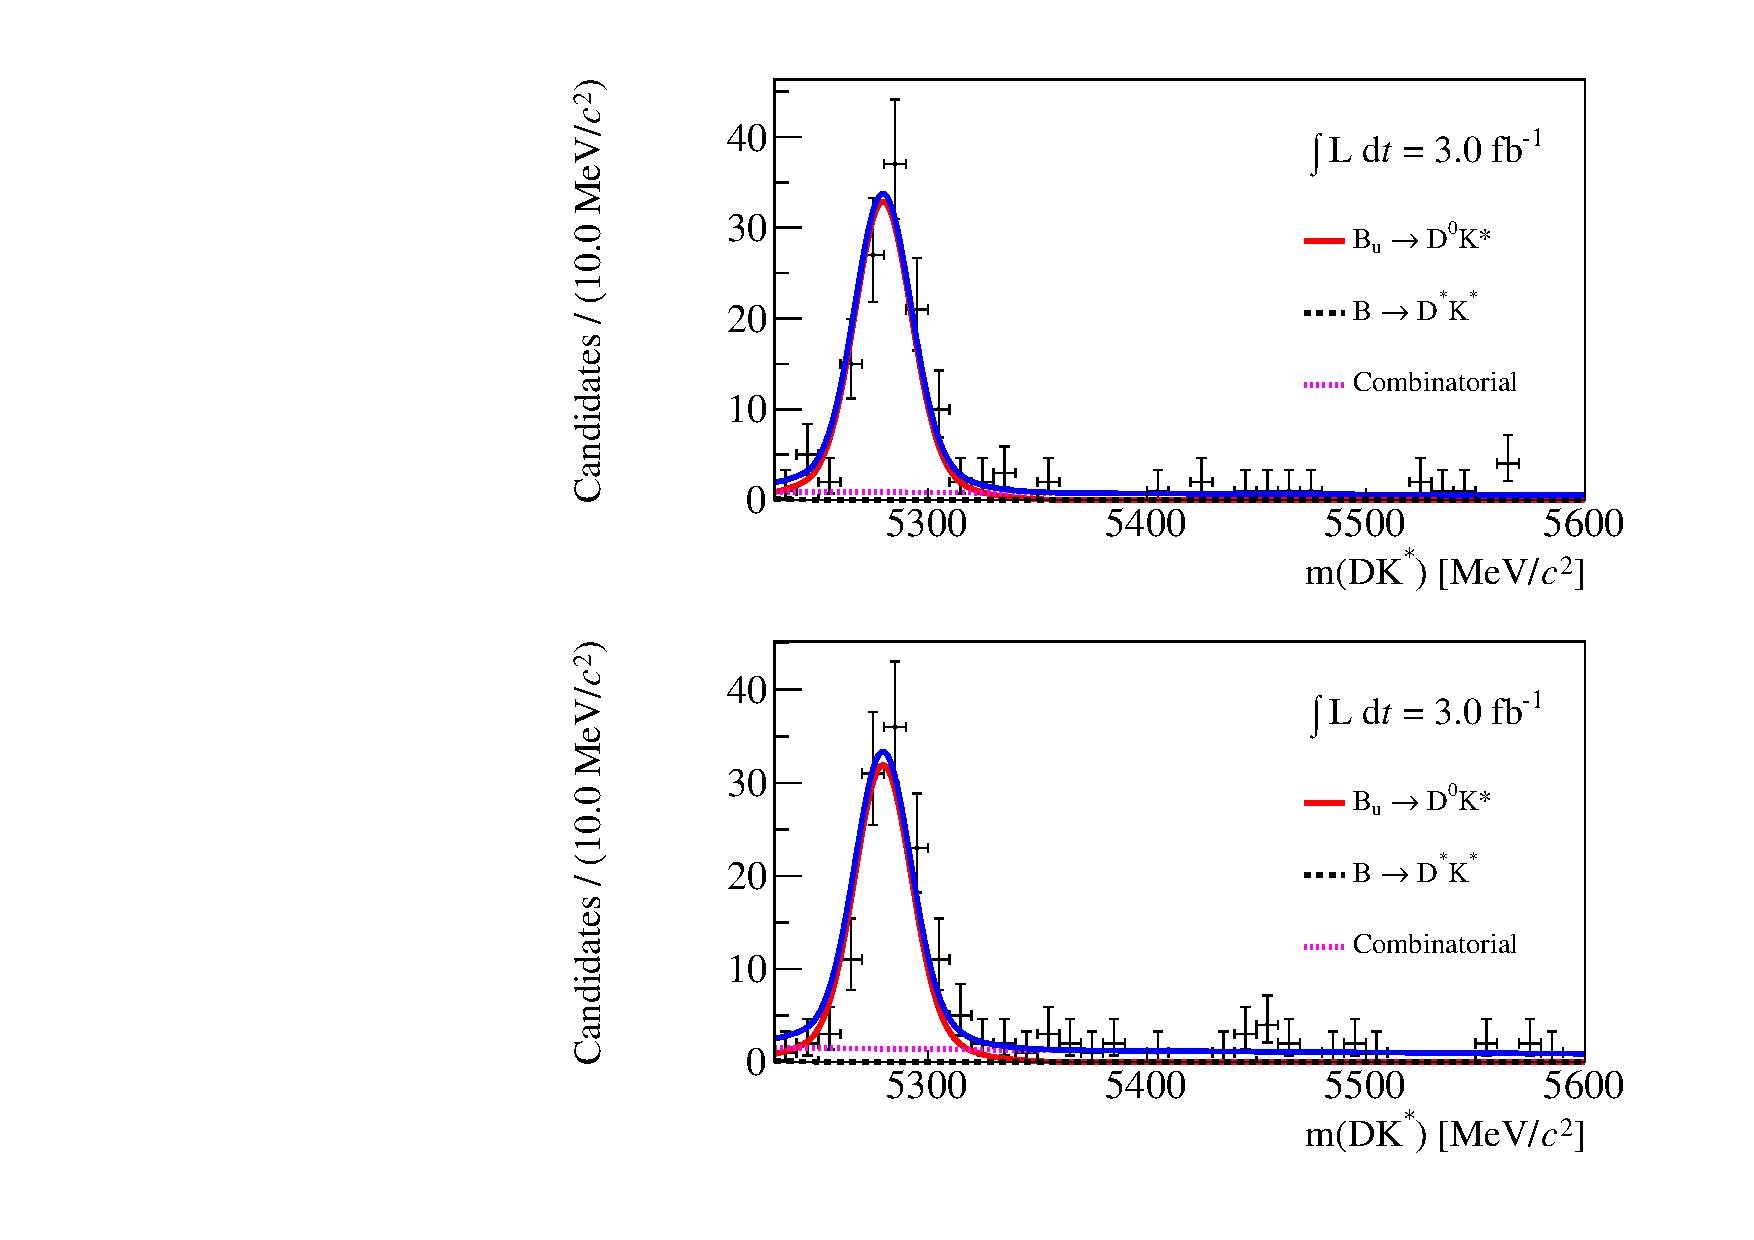
\includegraphics[width=0.3\linewidth]{figures/results/canvas_d2kpipipi_DD_run1.pdf}}
\hfill
\subfloat[$\pi\pi\pi\pi$, DD]{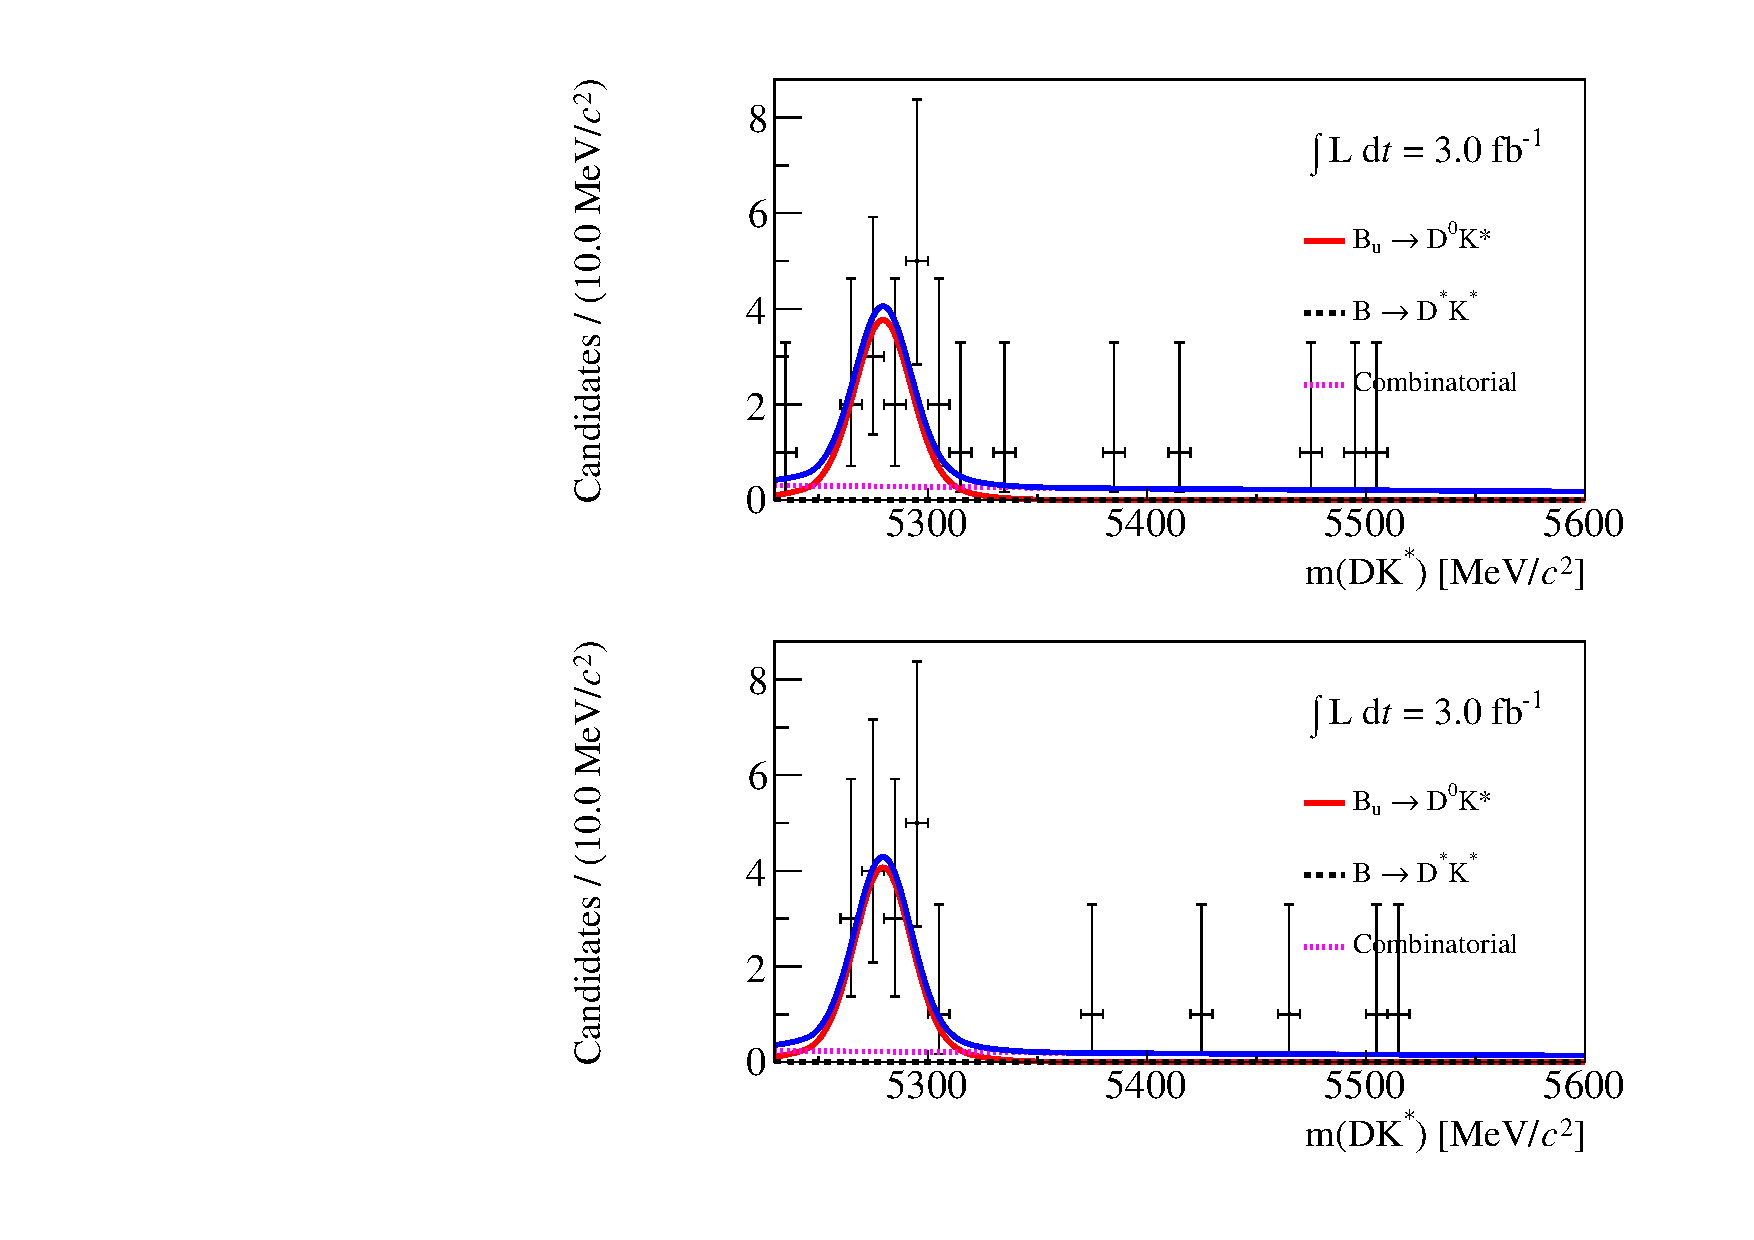
\includegraphics[width=0.3\linewidth]{figures/results/canvas_d2pipipipi_DD_run1.pdf}}
\hfill
\subfloat[$\pi K\pi\pi$, DD]{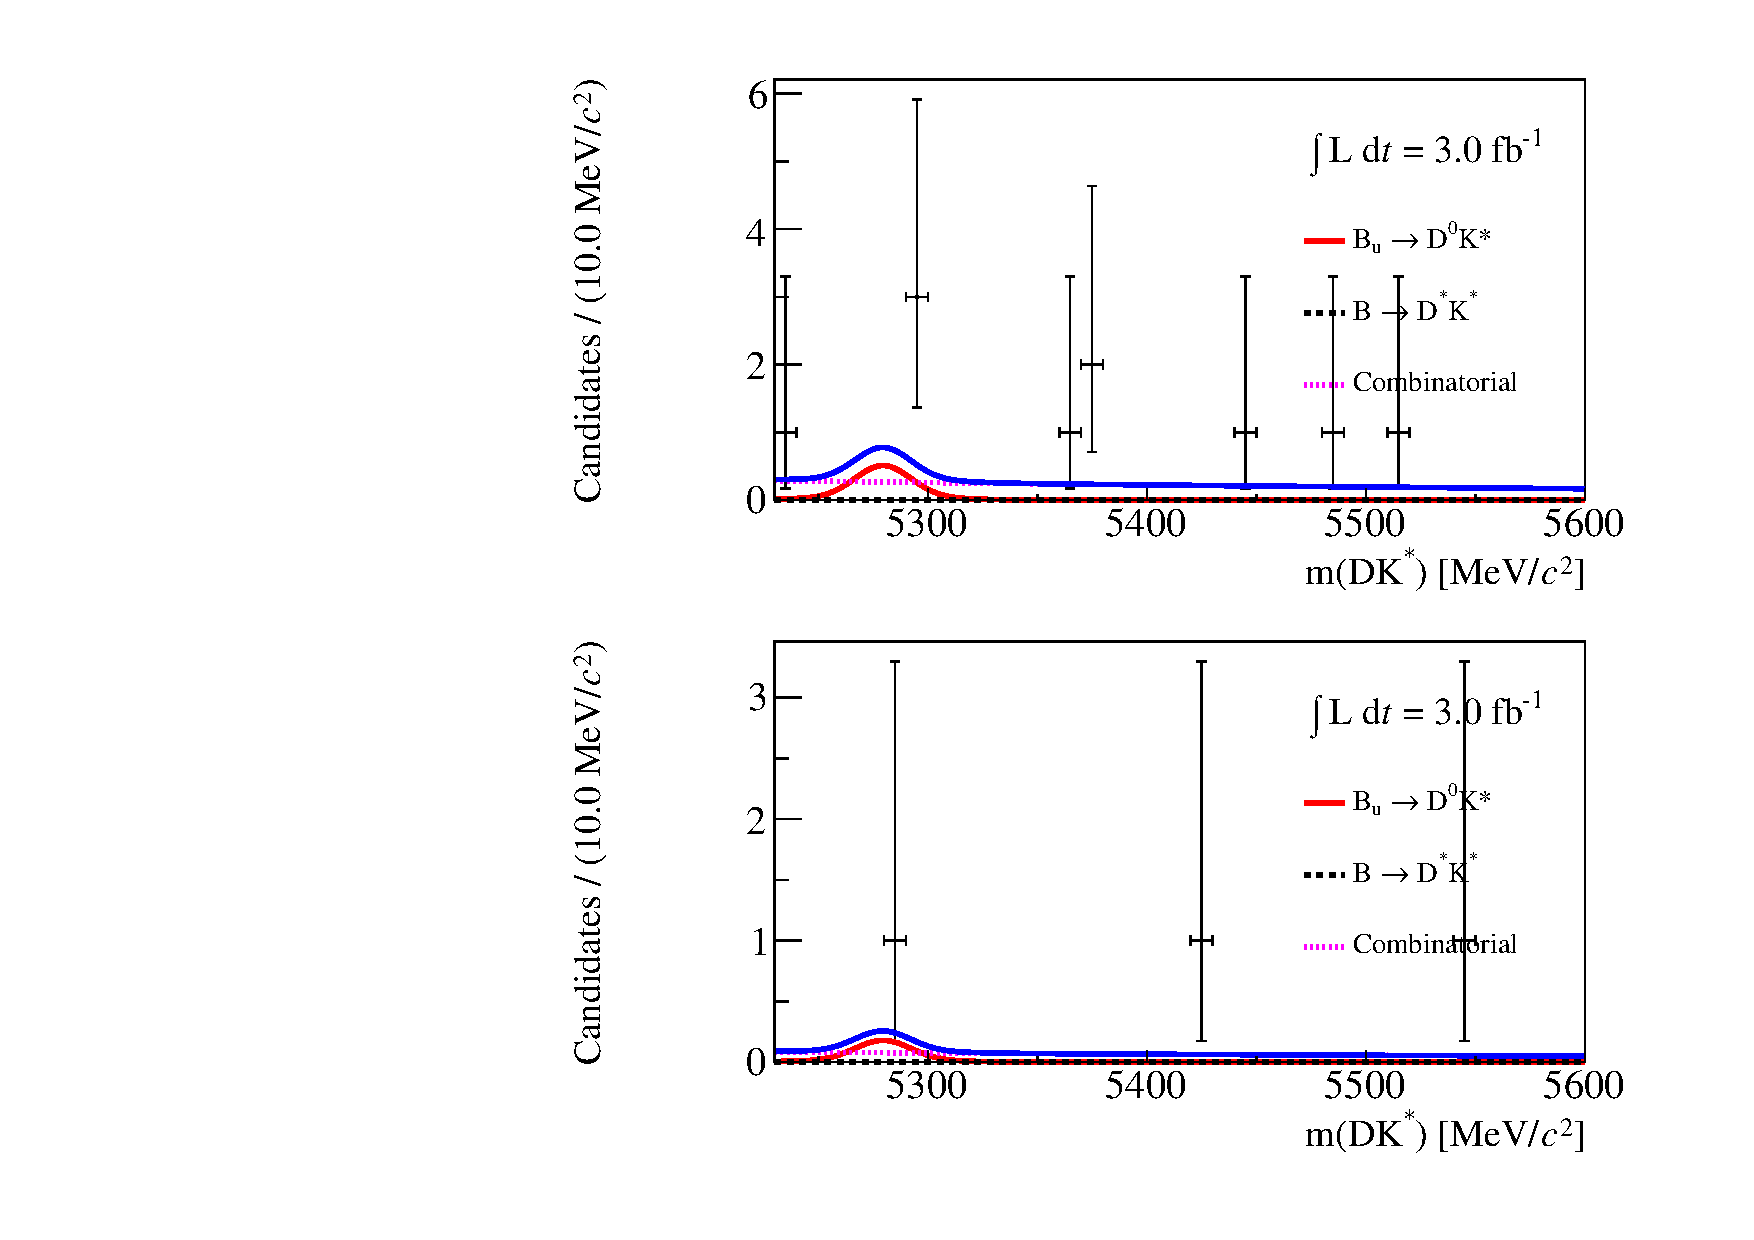
\includegraphics[width=0.3\linewidth]{figures/results/canvas_d2pikpipi_DD_run1.pdf}}
\caption{Results of the simultaneous fit for \runone data for four-body modes. In each pair the top plot is for \Bp decays and the bottom plot is for \Bm decays.}
\label{datafit4bodyRun1}
\end{sidewaysfigure}

\begin{sidewaysfigure}[h]
\centering
\subfloat[$K\pi$, LL]{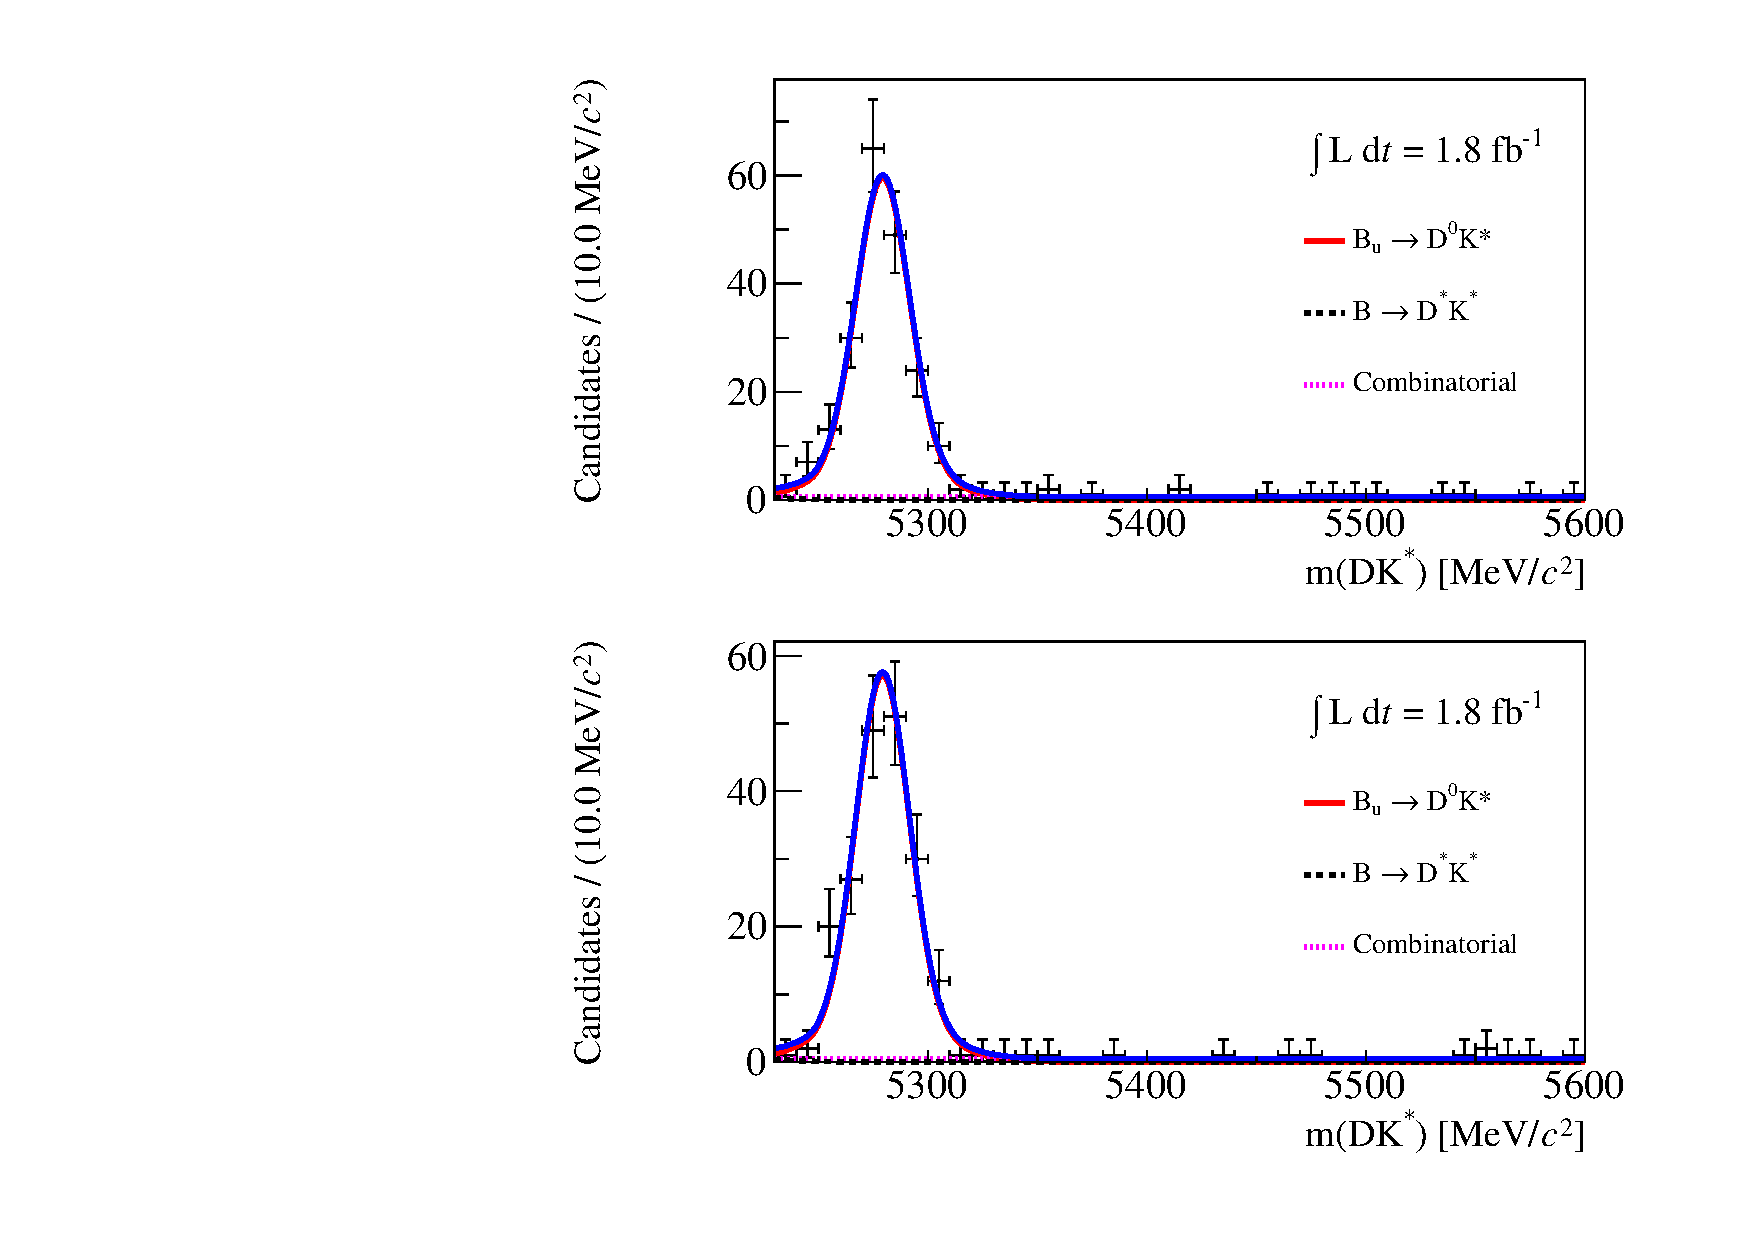
\includegraphics[width=0.25\linewidth]{figures/results/canvas_d2kpi_LL_run2.pdf}}
\hfill
\subfloat[$KK$, LL]{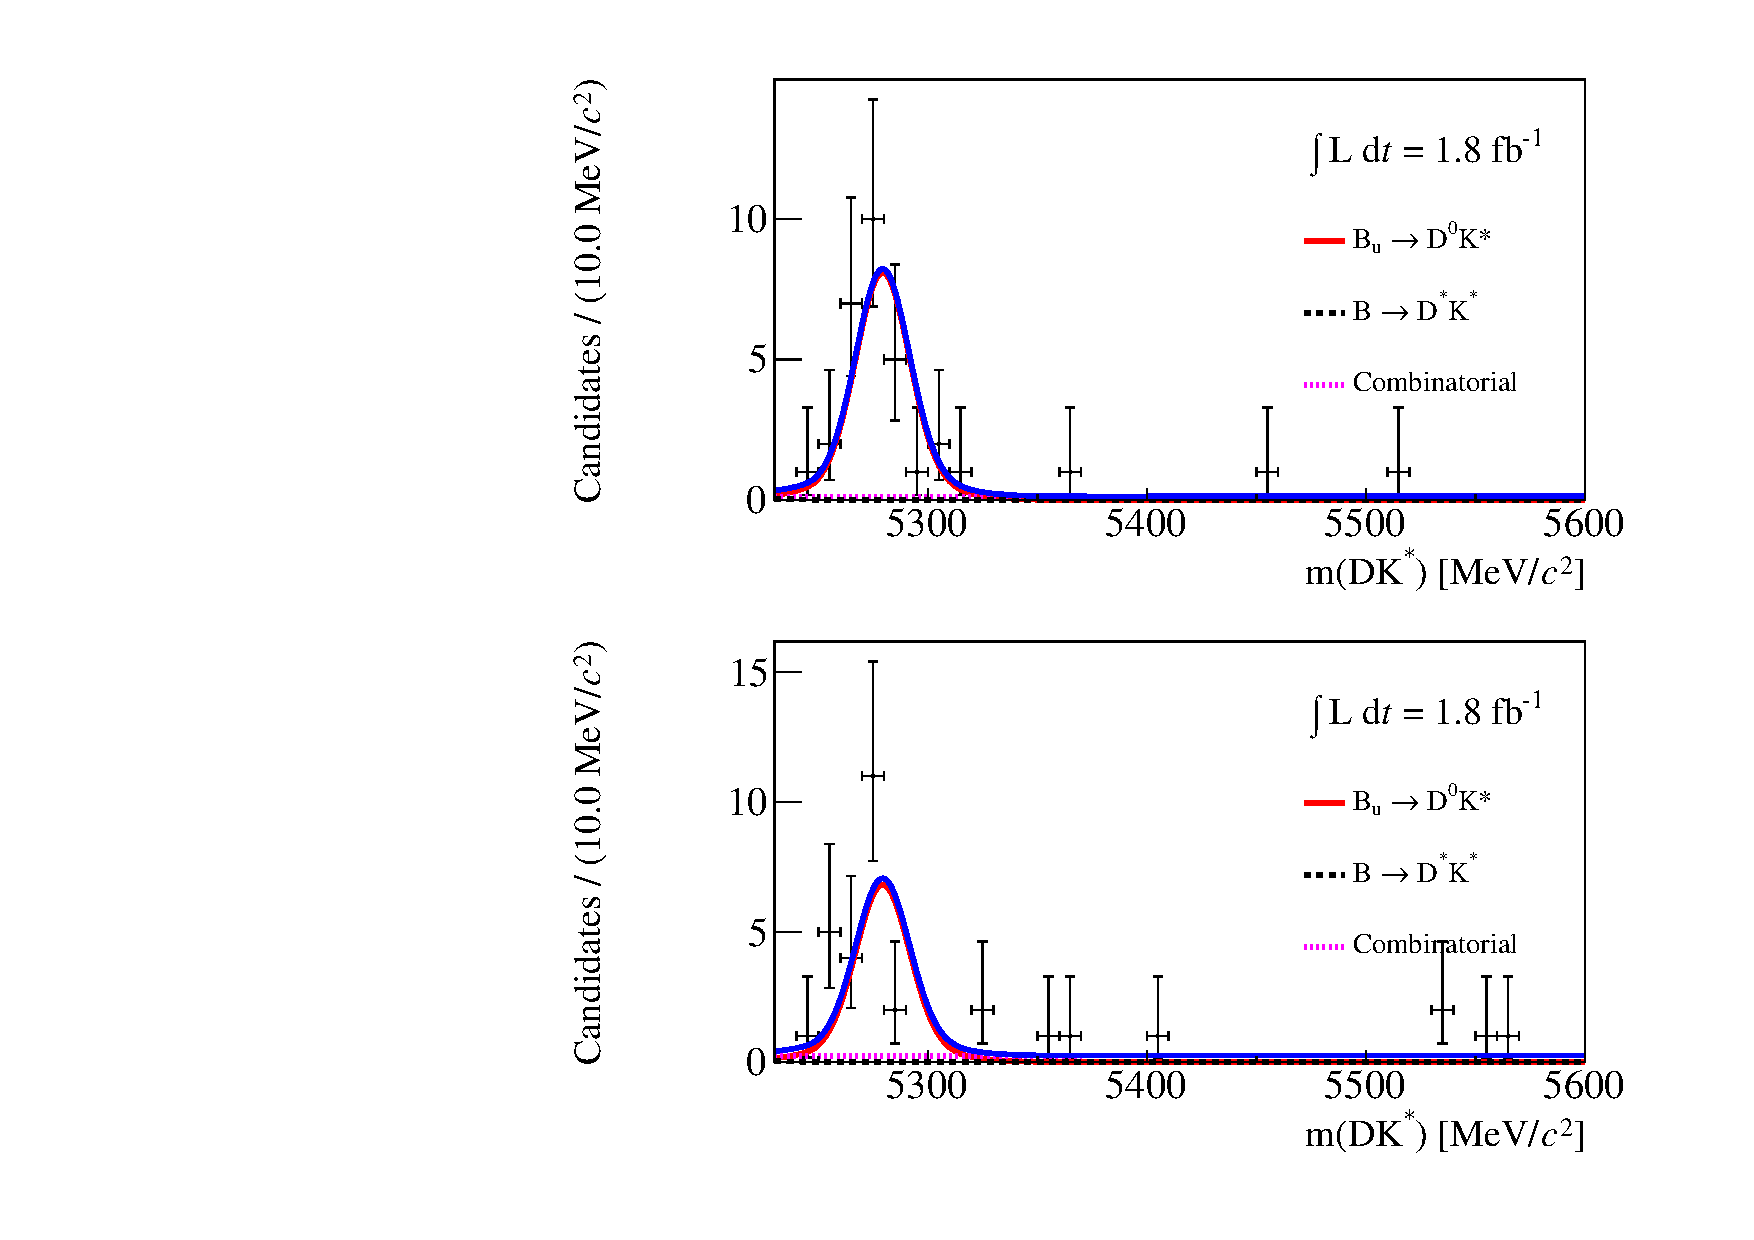
\includegraphics[width=0.25\linewidth]{figures/results/canvas_d2kk_LL_run2.pdf}}
\hfill
\subfloat[$\pi\pi$, LL]{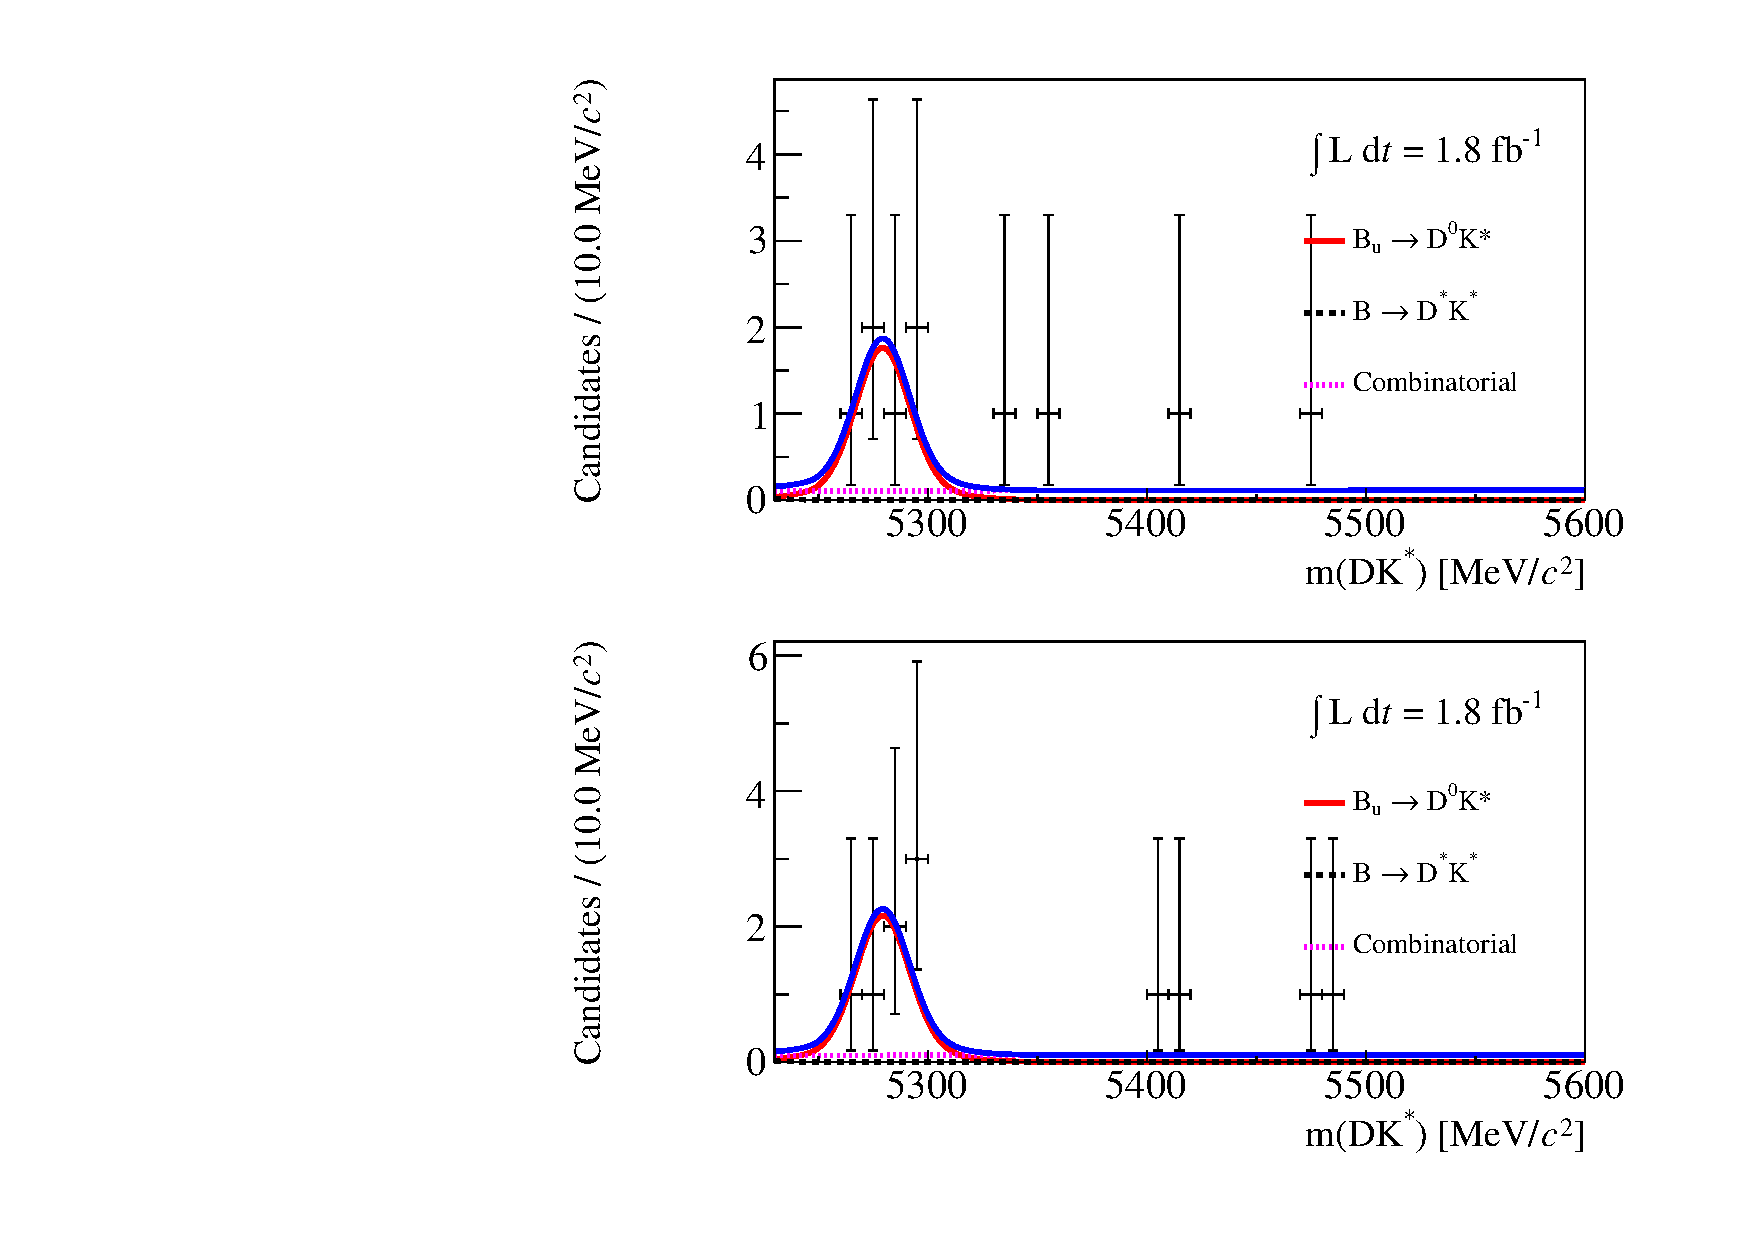
\includegraphics[width=0.25\linewidth]{figures/results/canvas_d2pipi_LL_run2.pdf}}
\hfill
\subfloat[$\pi K$, LL]{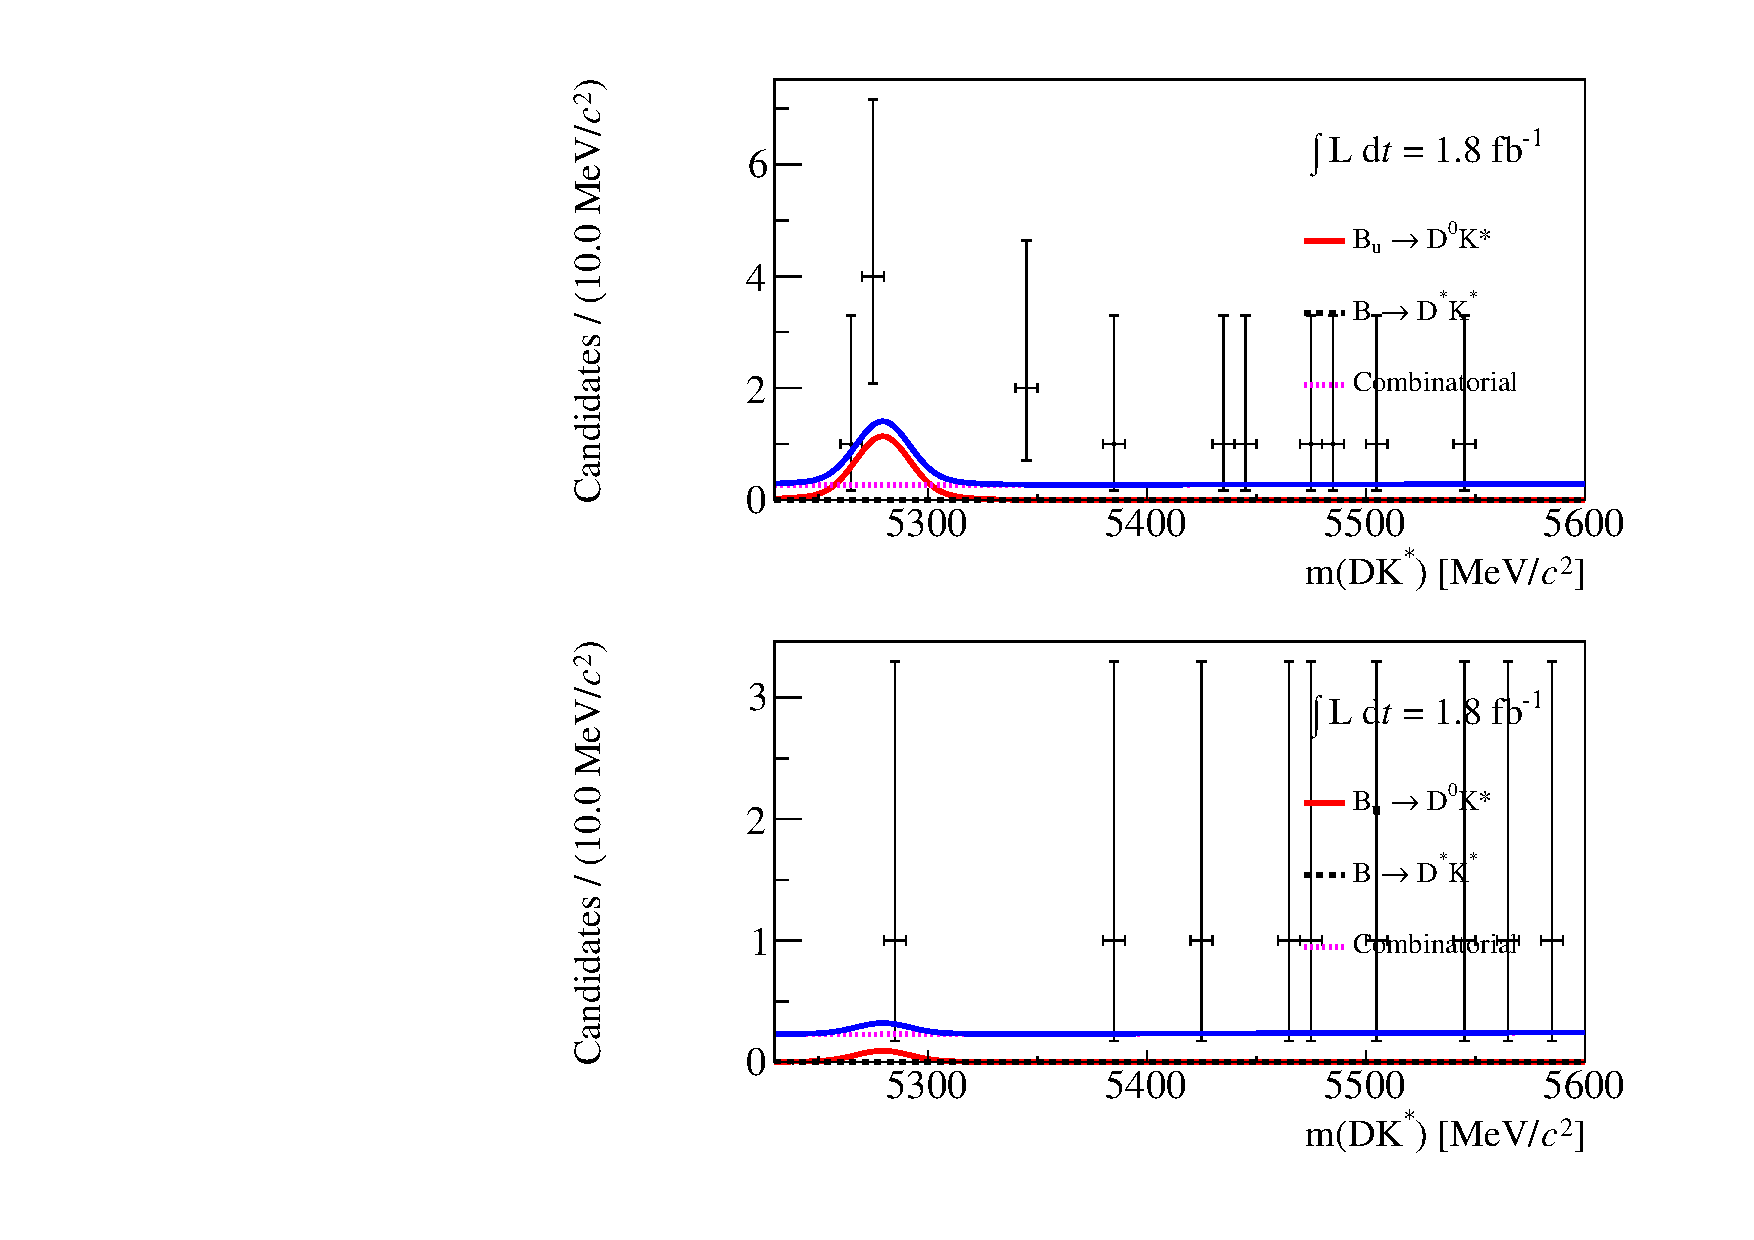
\includegraphics[width=0.25\linewidth]{figures/results/canvas_d2pik_LL_run2.pdf}}
\hfill
\subfloat[$K\pi$, DD]{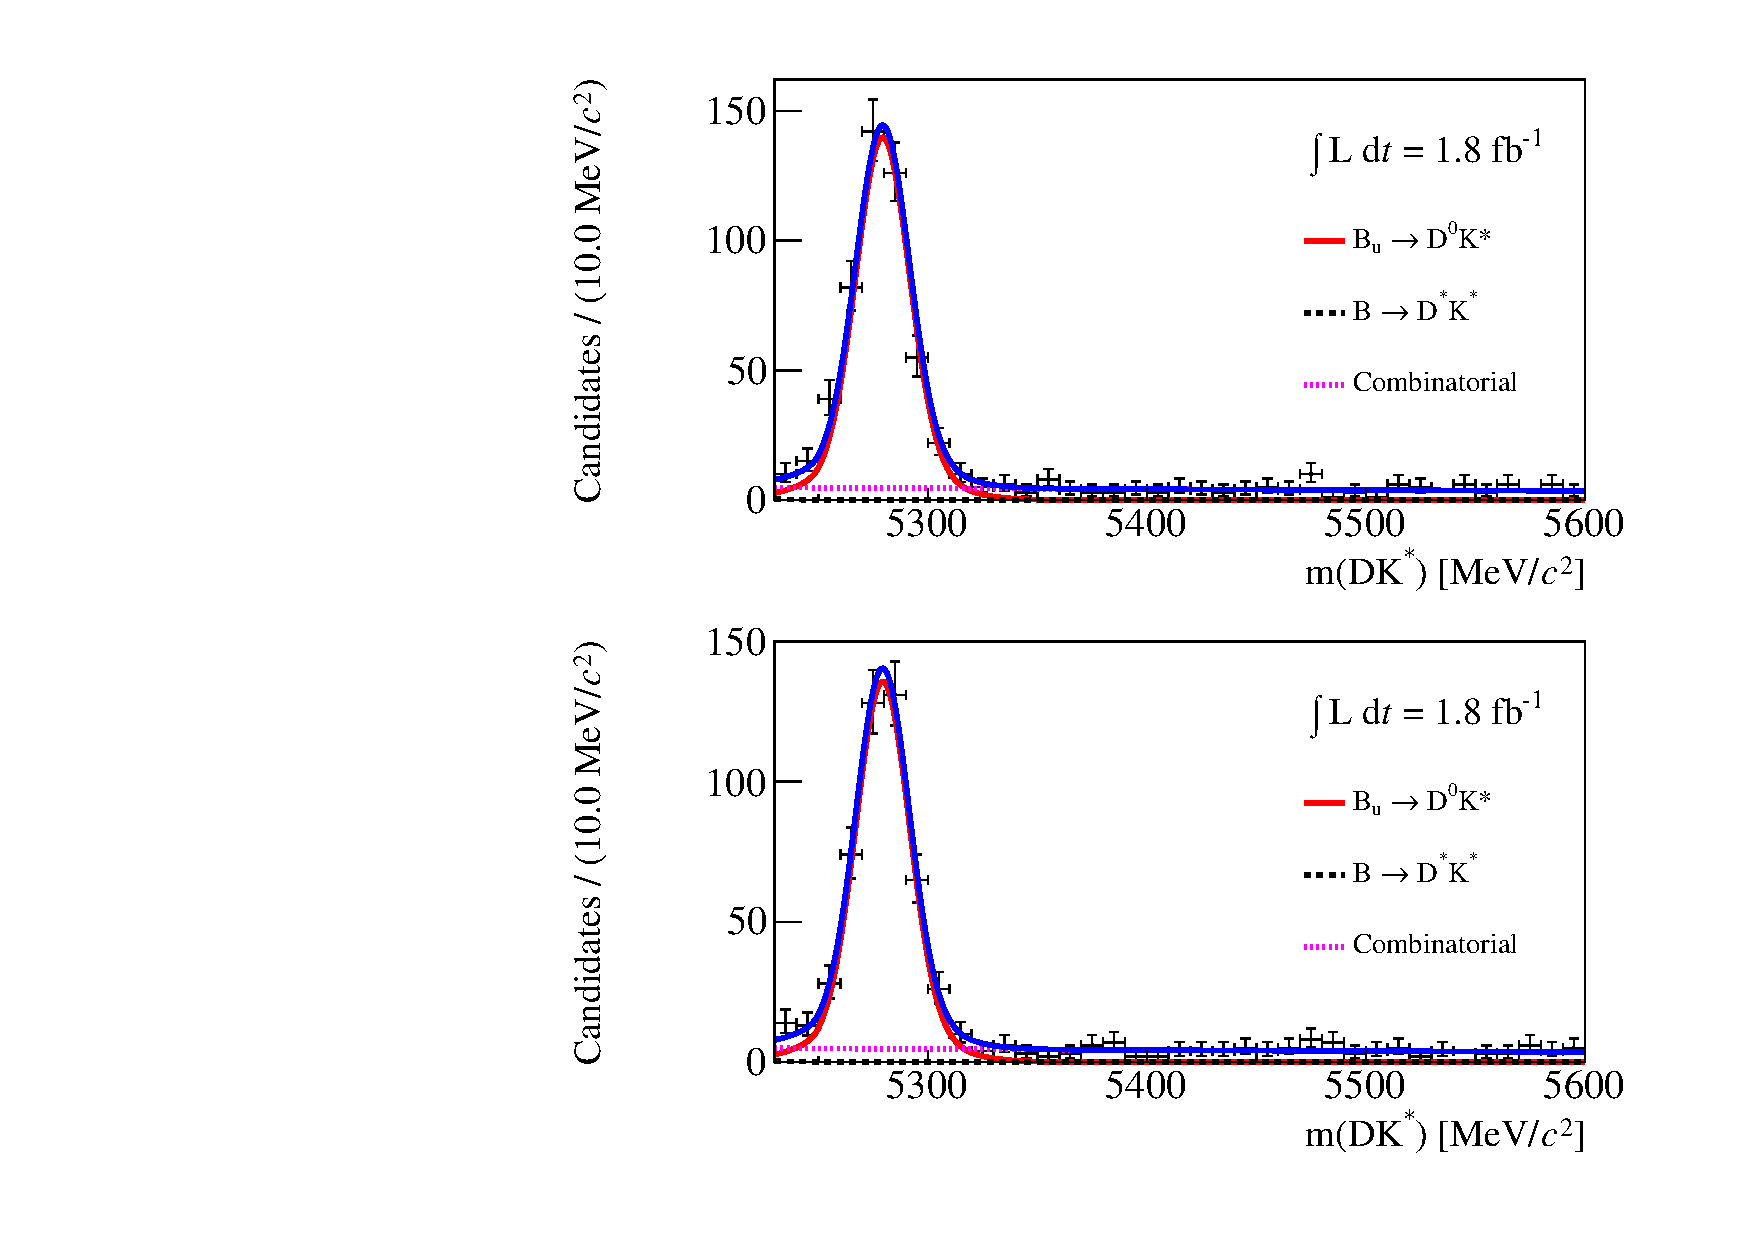
\includegraphics[width=0.25\linewidth]{figures/results/canvas_d2kpi_DD_run2.pdf}}
\hfill
\subfloat[$KK$, DD]{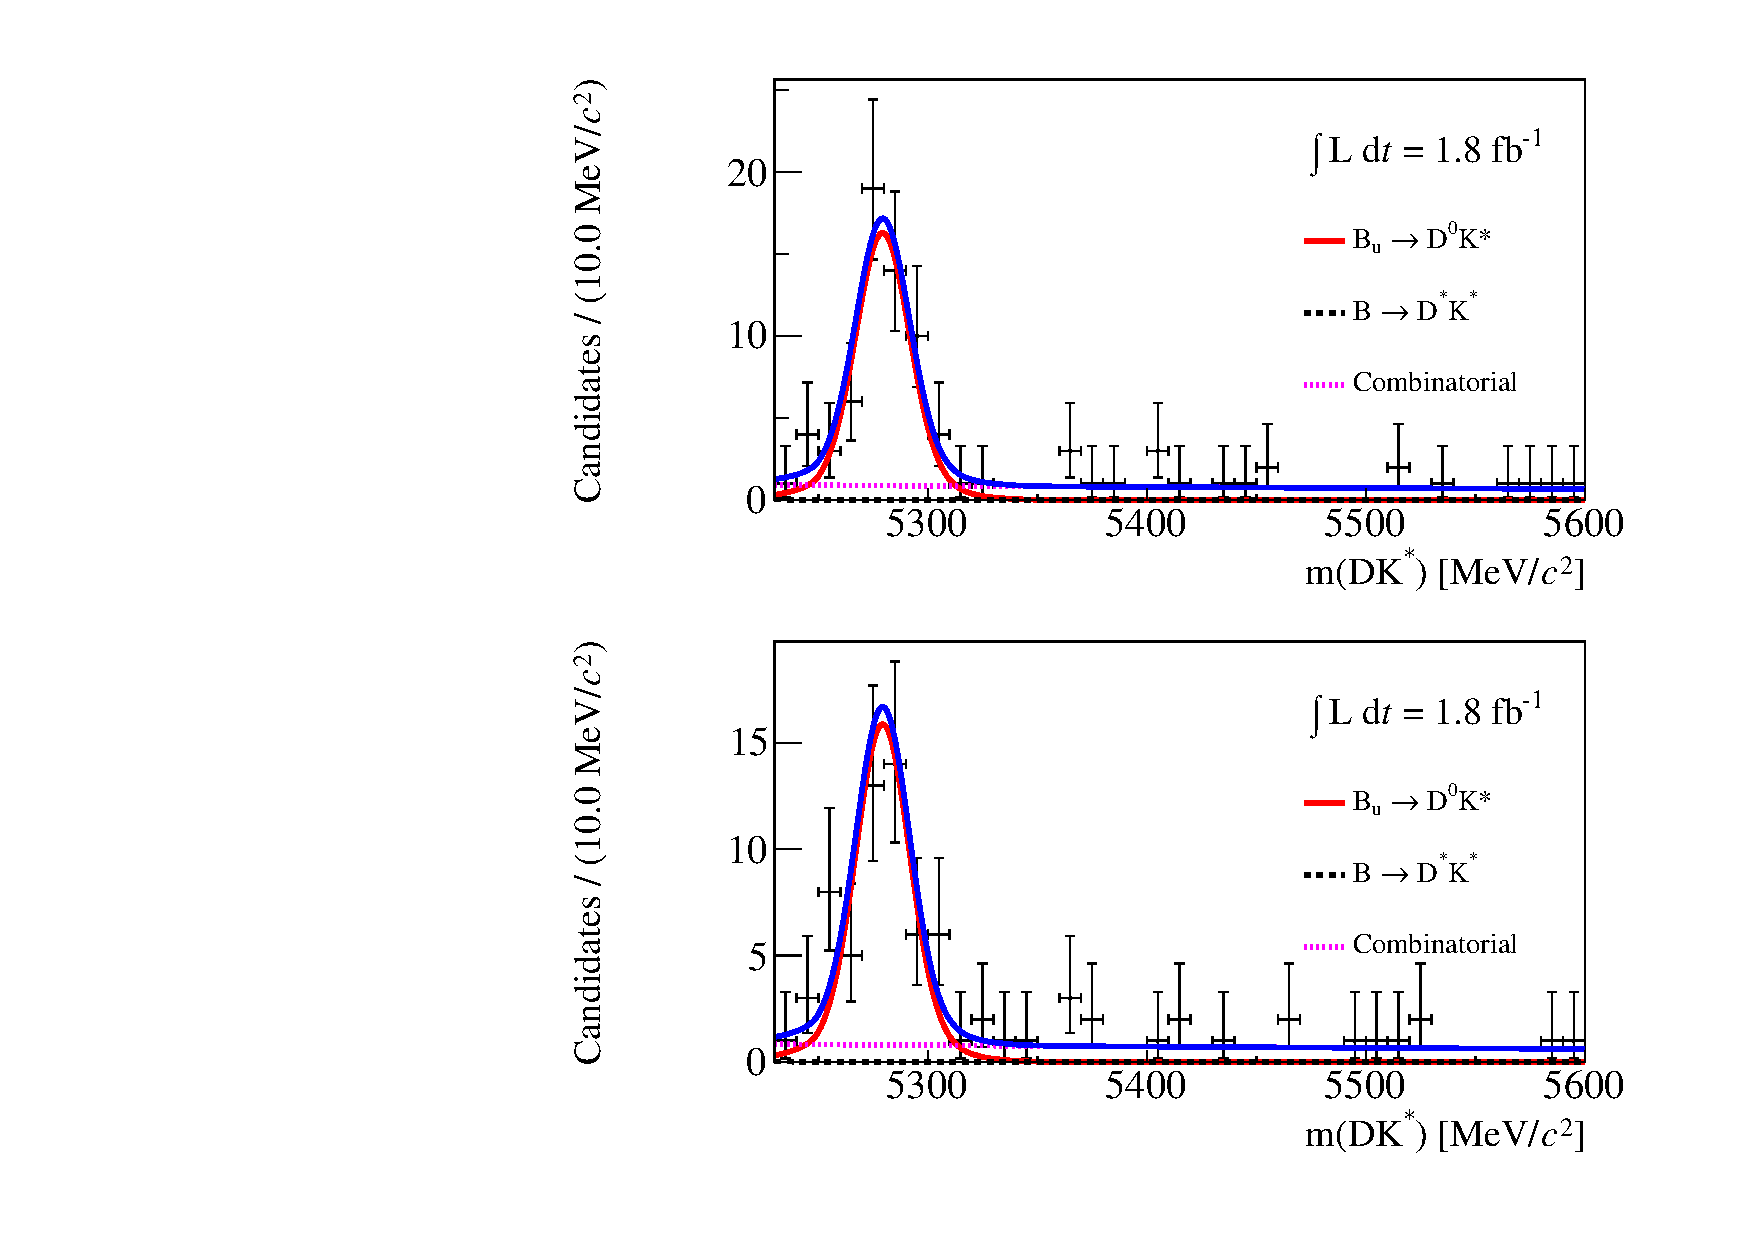
\includegraphics[width=0.25\linewidth]{figures/results/canvas_d2kk_DD_run2.pdf}}
\hfill
\subfloat[$\pi\pi$, DD]{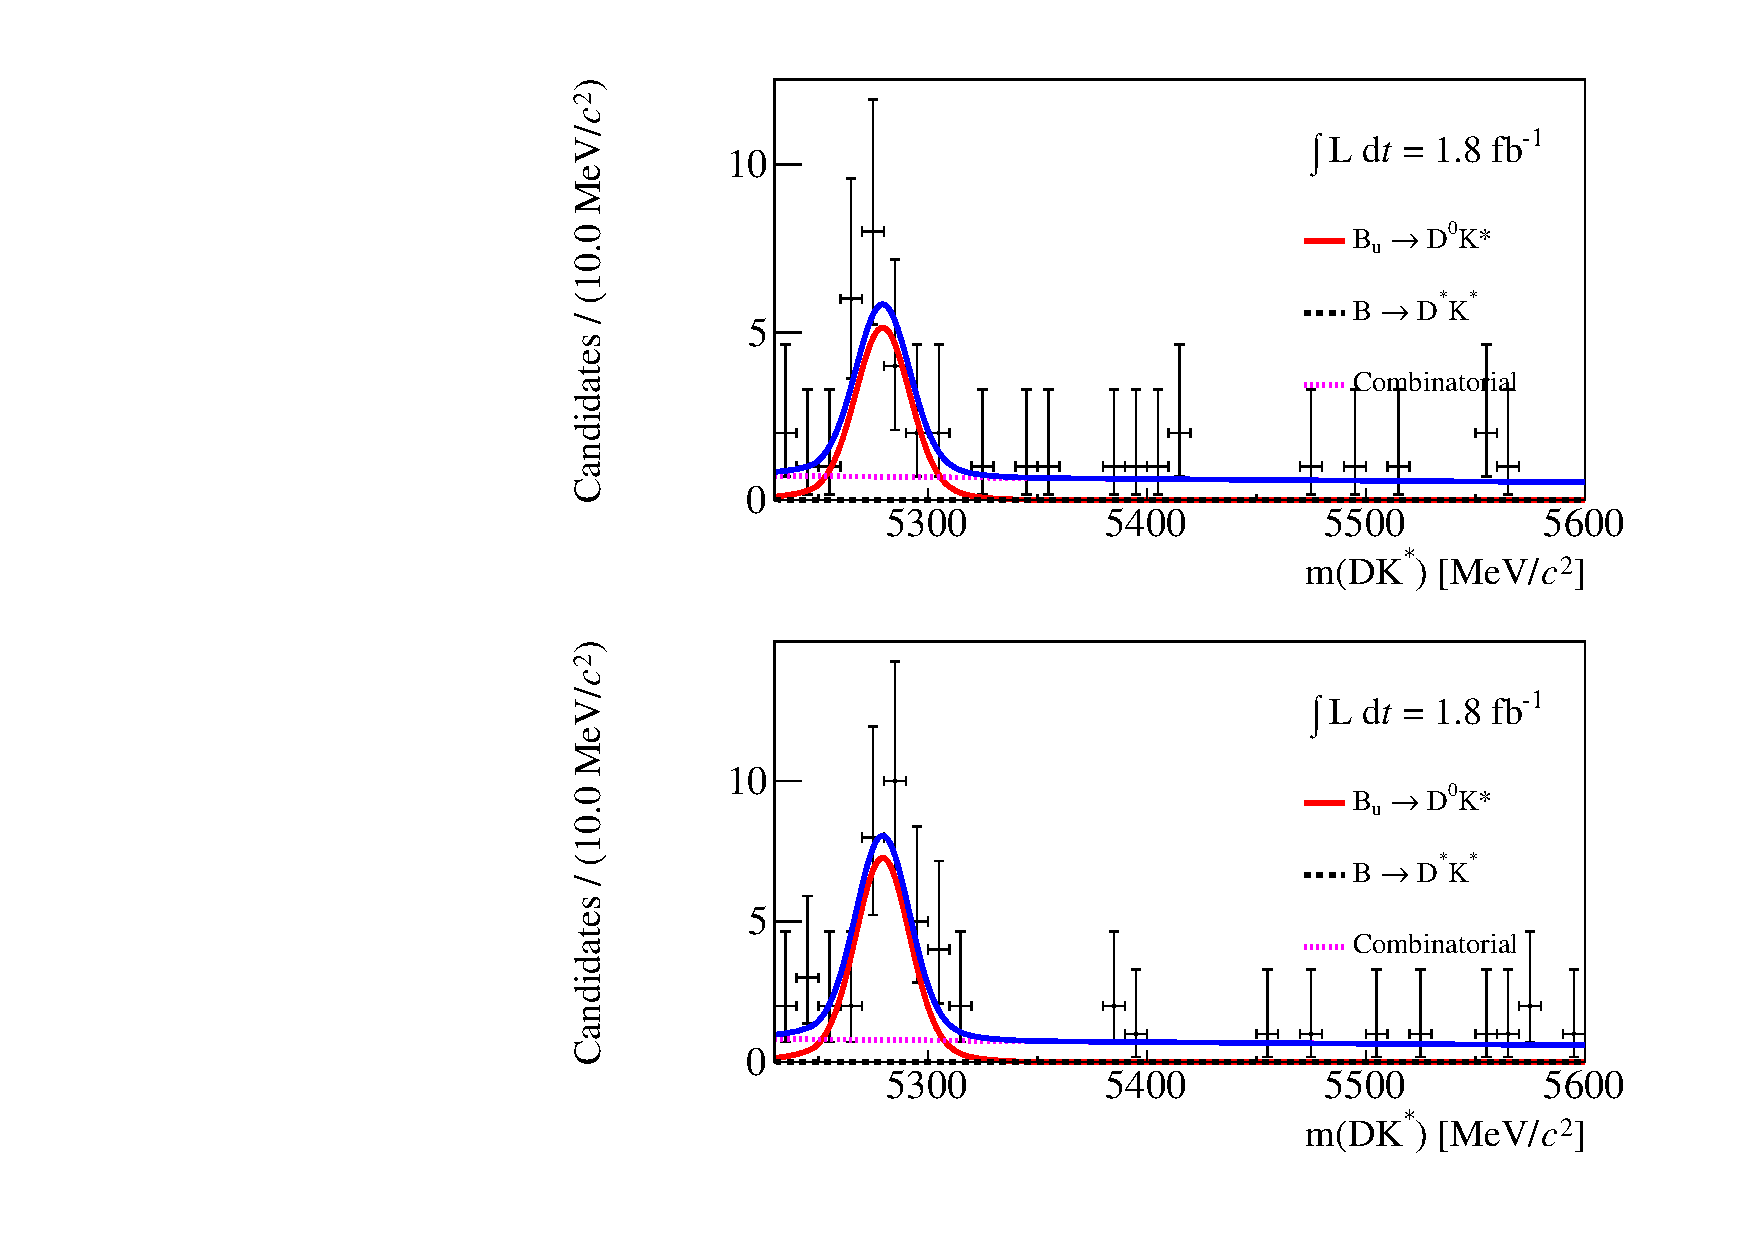
\includegraphics[width=0.25\linewidth]{figures/results/canvas_d2pipi_DD_run2.pdf}}
\hfill
\subfloat[$\pi K$, DD]{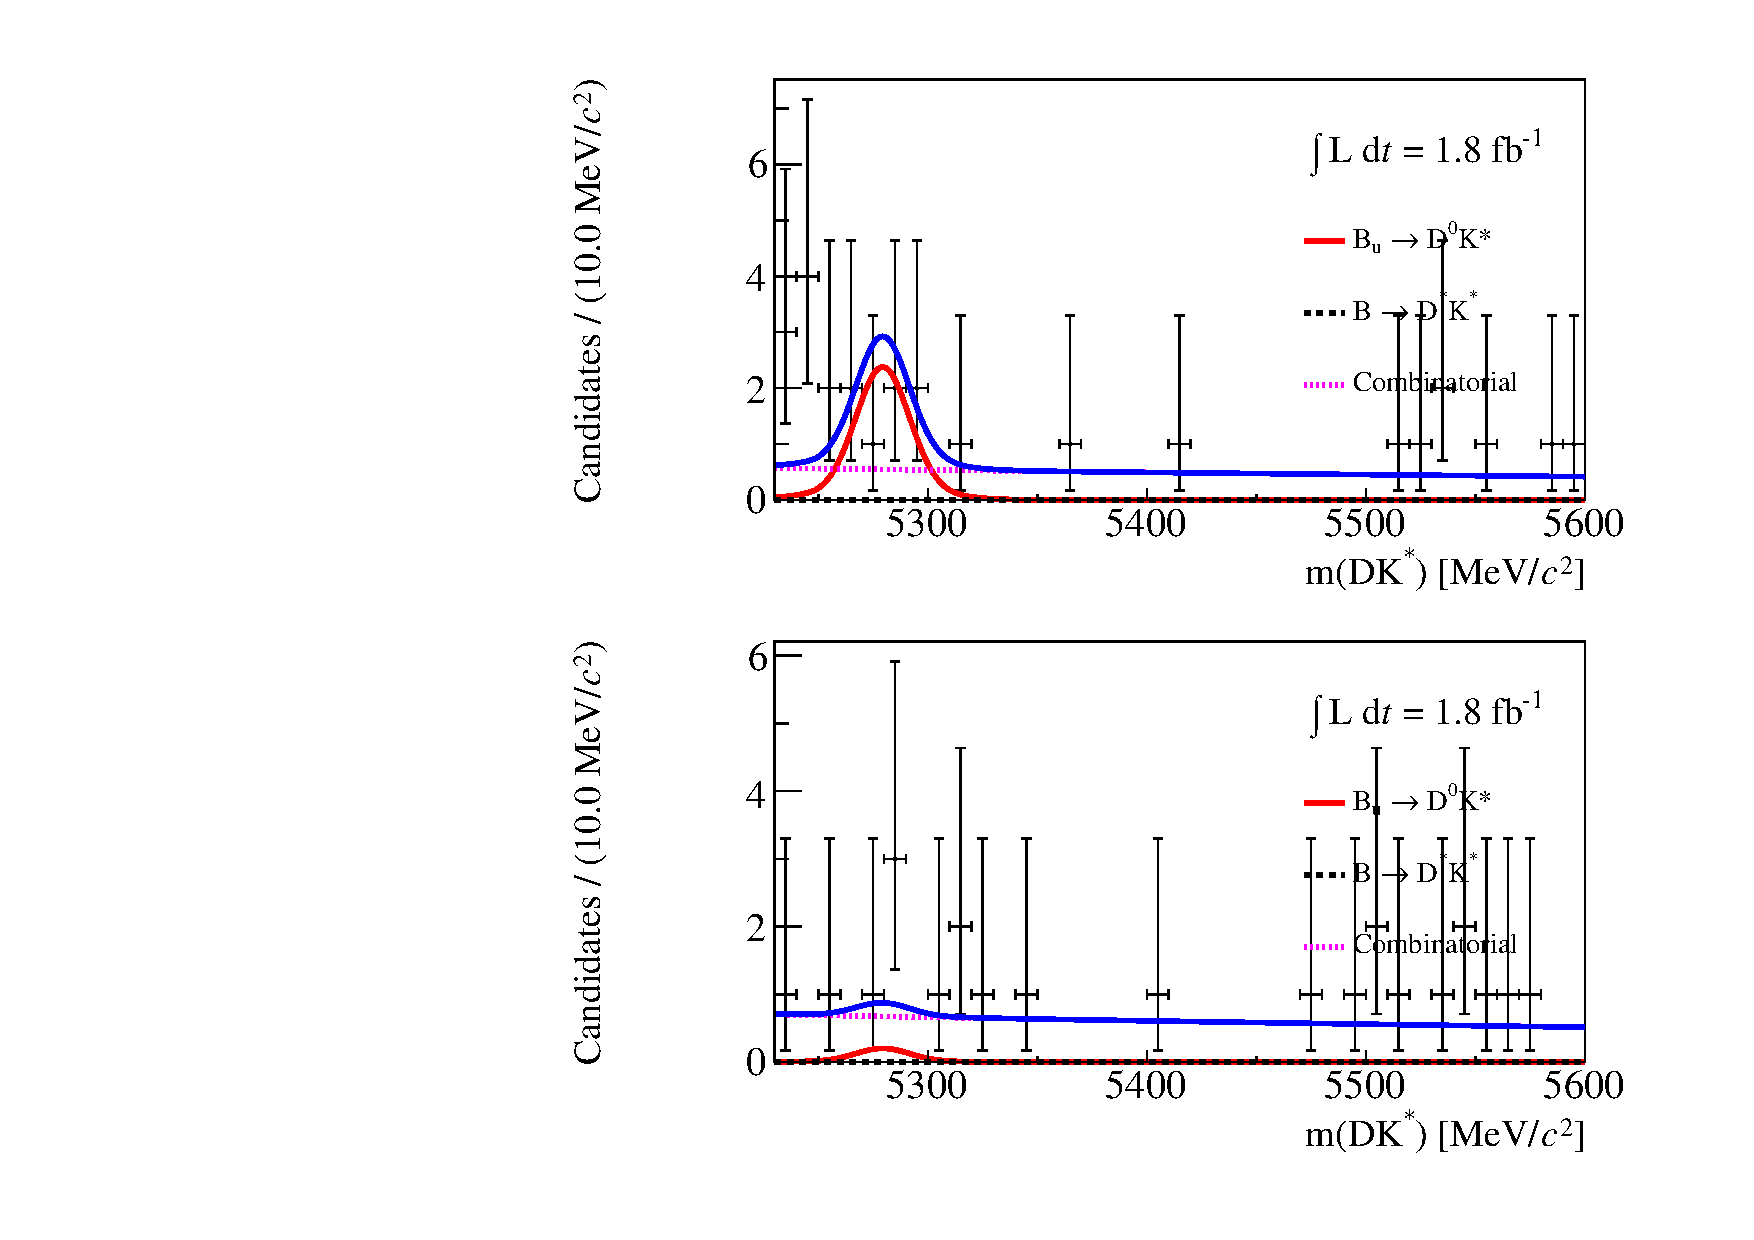
\includegraphics[width=0.25\linewidth]{figures/results/canvas_d2pik_DD_run2.pdf}}
\caption{Results of the simultaneous fit for \runtwo data for two-body modes. In each pair the top plot is for \Bp decays and the bottom plot is for \Bm decays.}
\label{datafit2bodyRun2}
\end{sidewaysfigure}

\begin{sidewaysfigure}[h]
\centering
\subfloat[$K\pi\pi\pi$, LL]{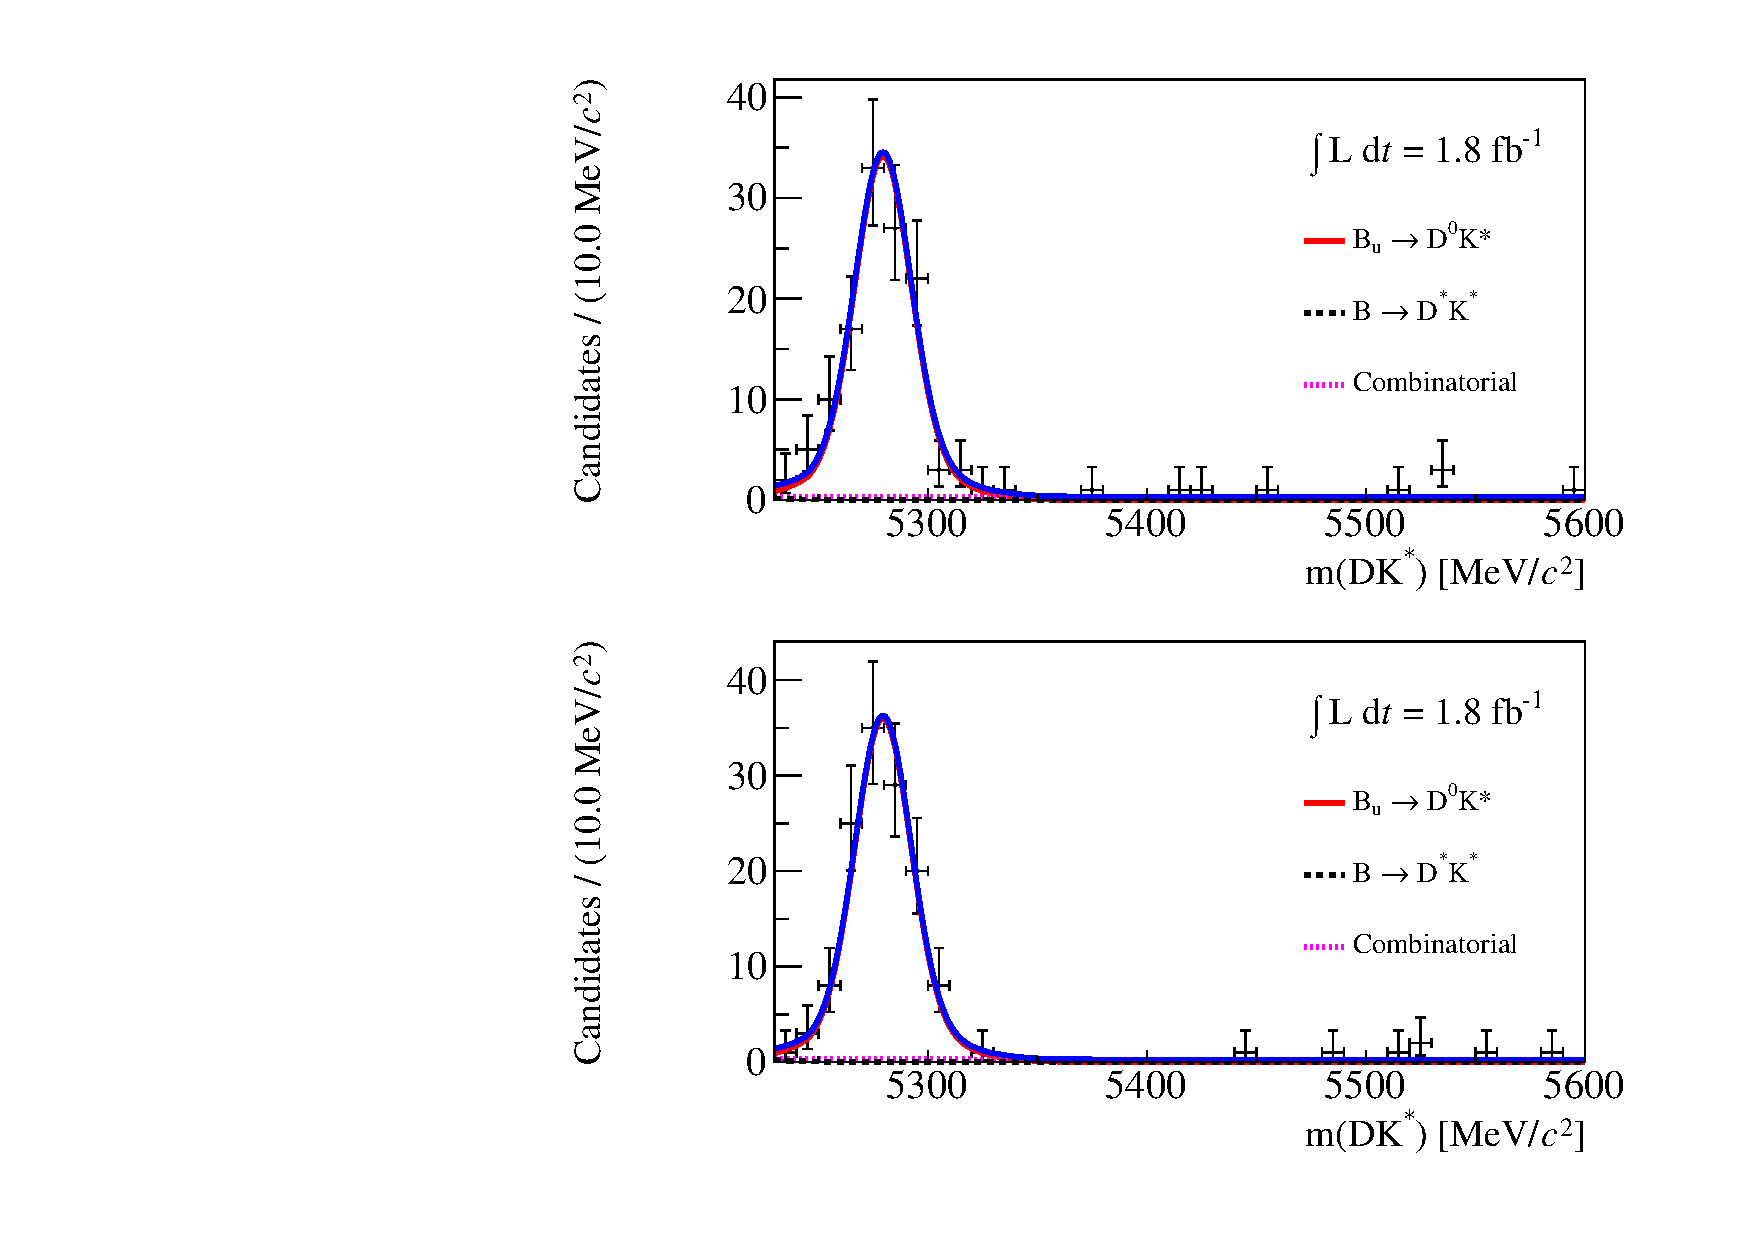
\includegraphics[width=0.3\linewidth]{figures/results/canvas_d2kpipipi_LL_run2.pdf}}
\hfill
\subfloat[$\pi\pi\pi\pi$, LL]{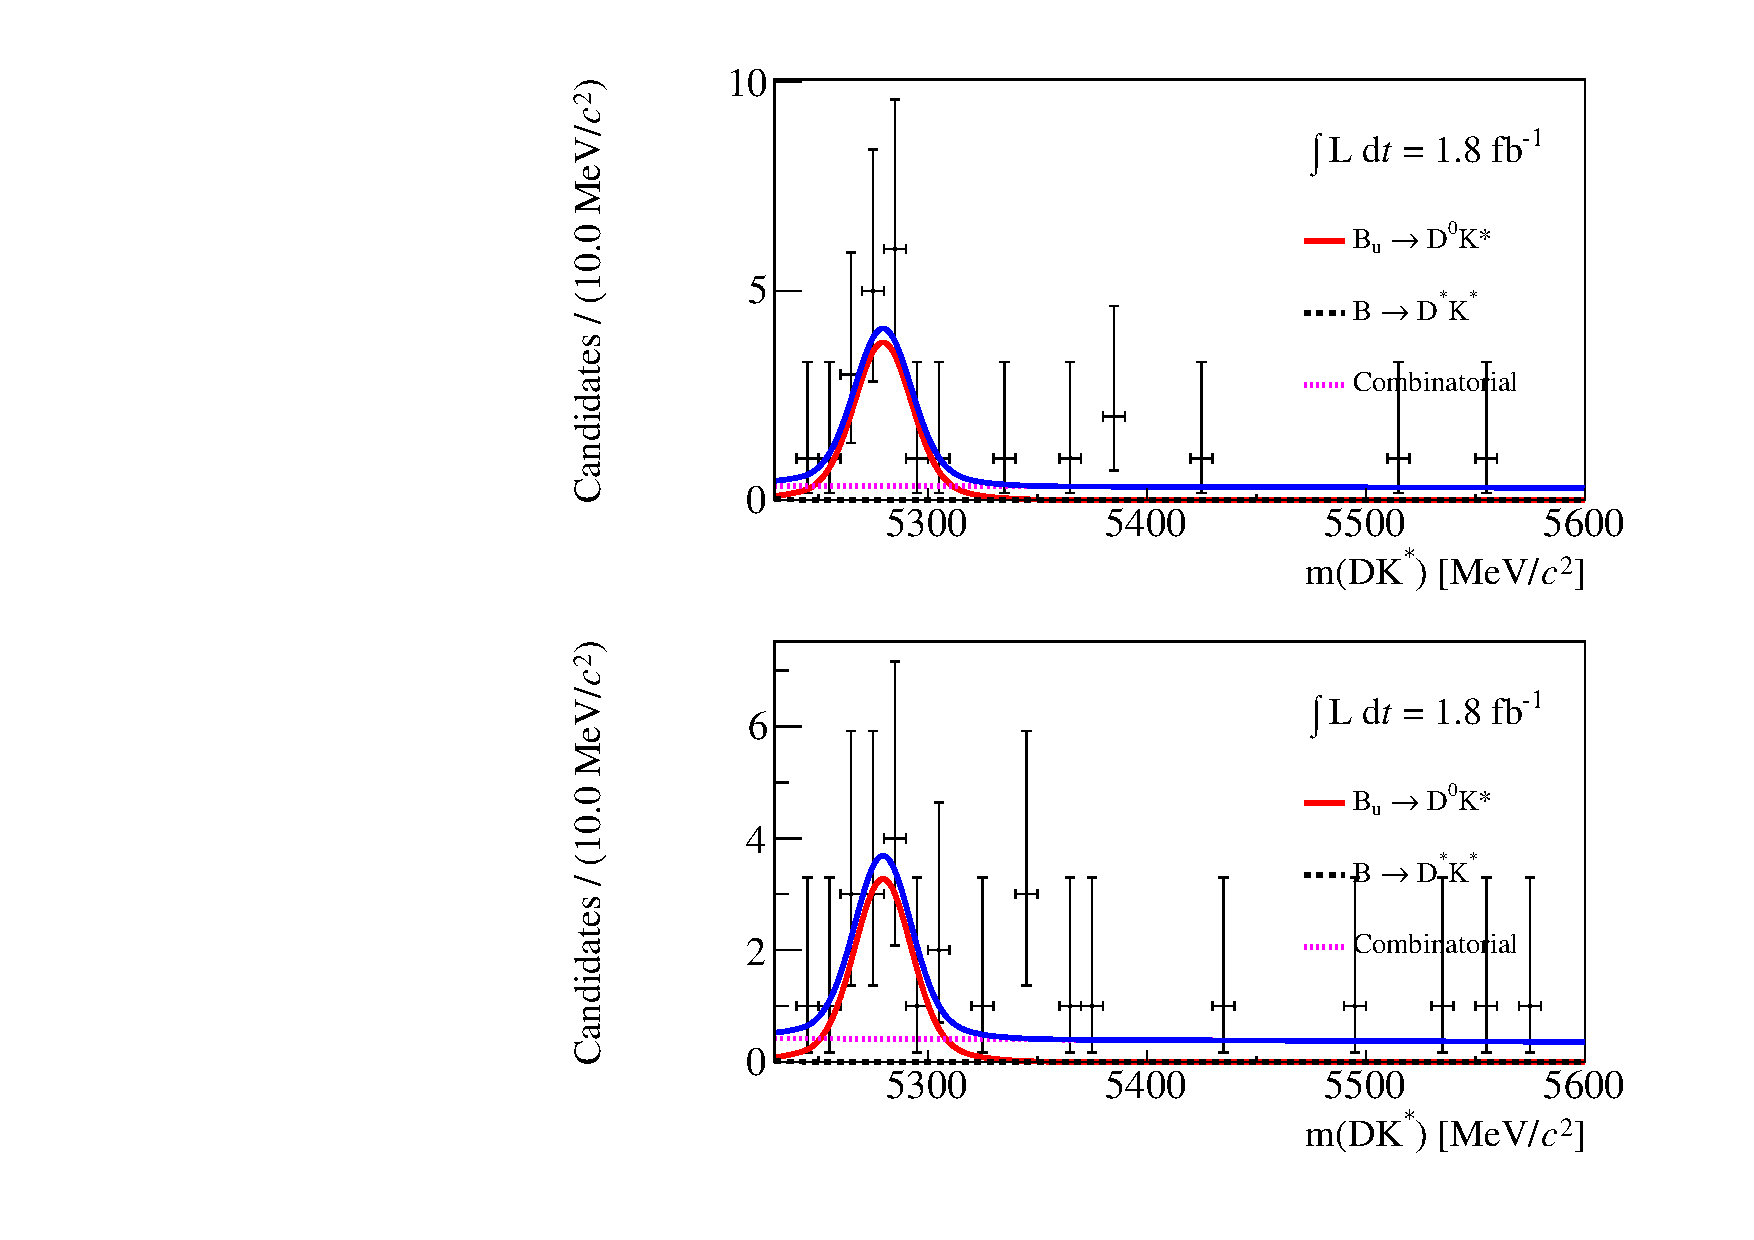
\includegraphics[width=0.3\linewidth]{figures/results/canvas_d2pipipipi_LL_run2.pdf}}
\hfill
\subfloat[$\pi K\pi\pi$, LL]{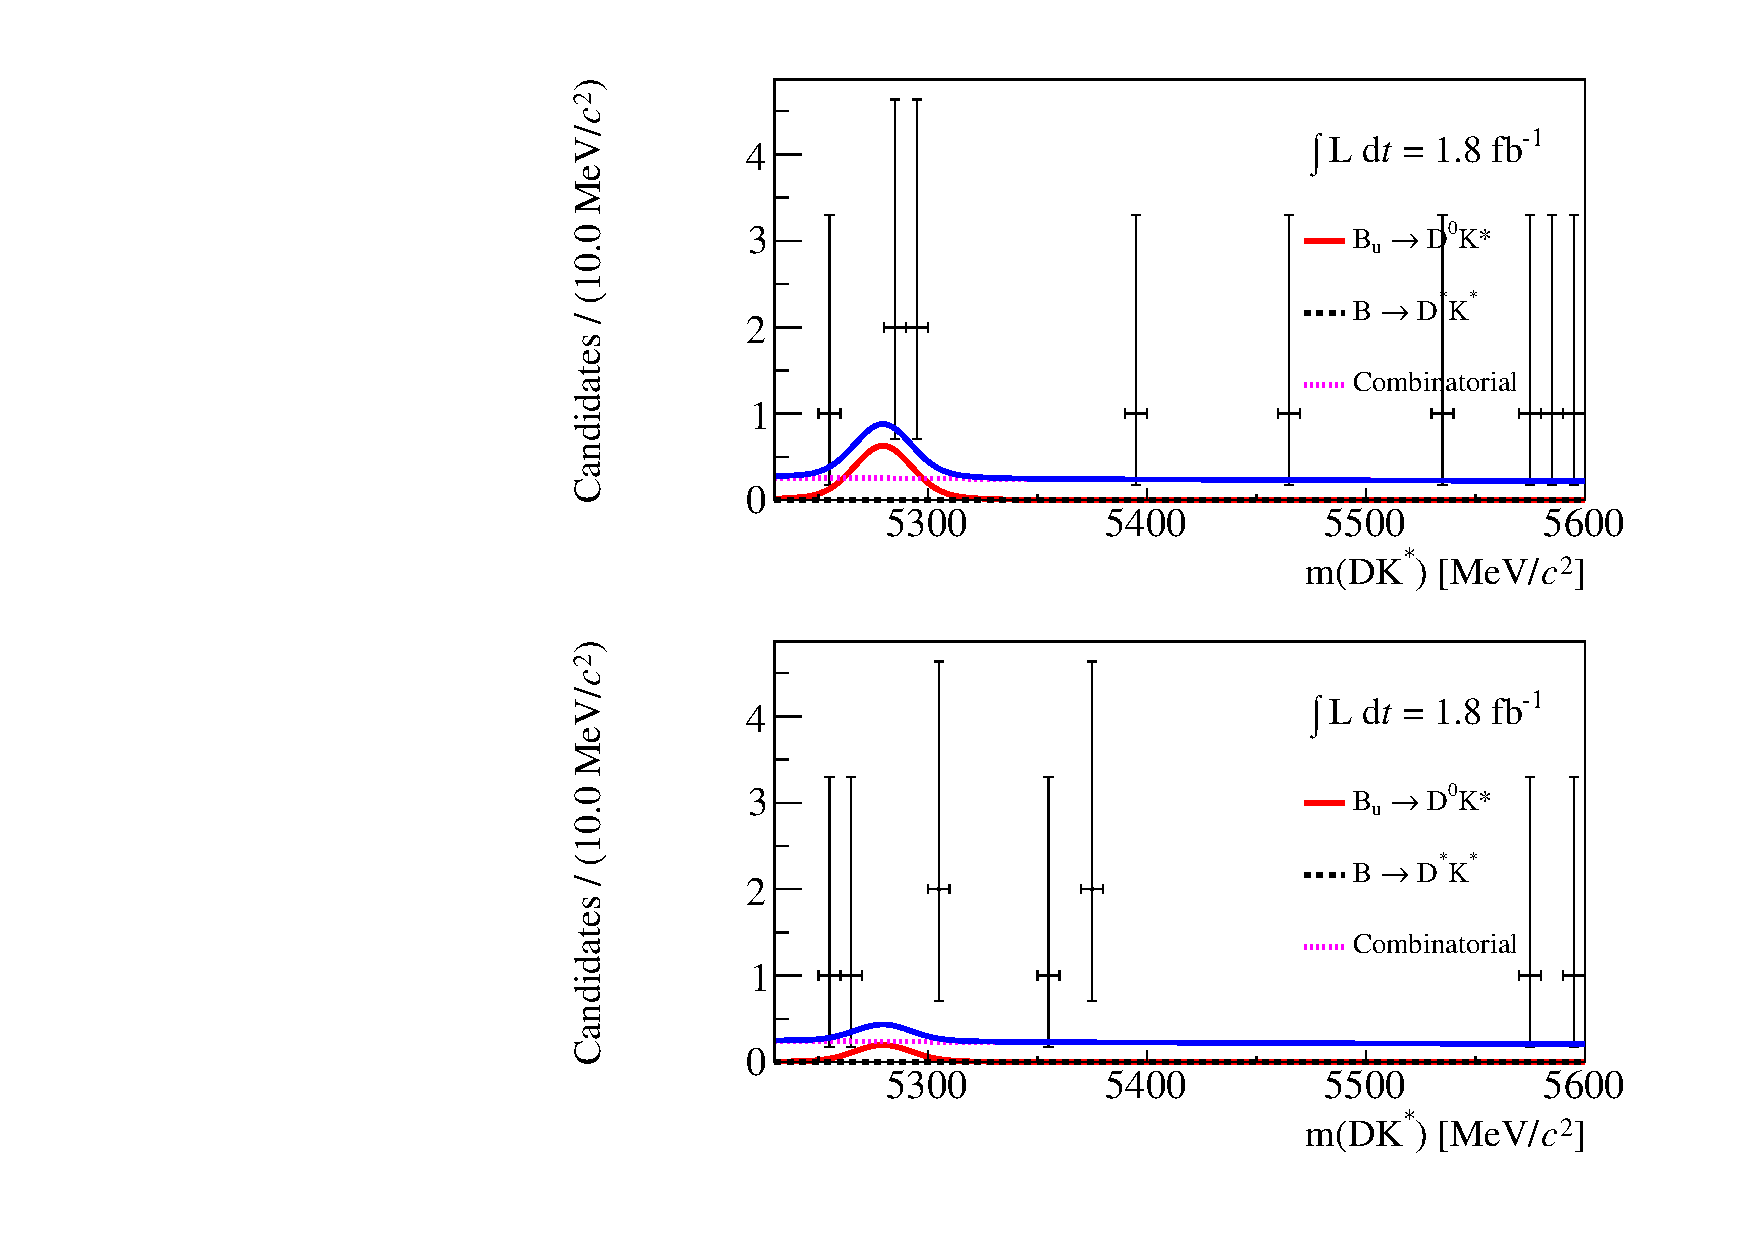
\includegraphics[width=0.3\linewidth]{figures/results/canvas_d2pikpipi_LL_run2.pdf}}
\hfill
\subfloat[$K\pi\pi\pi$, DD]{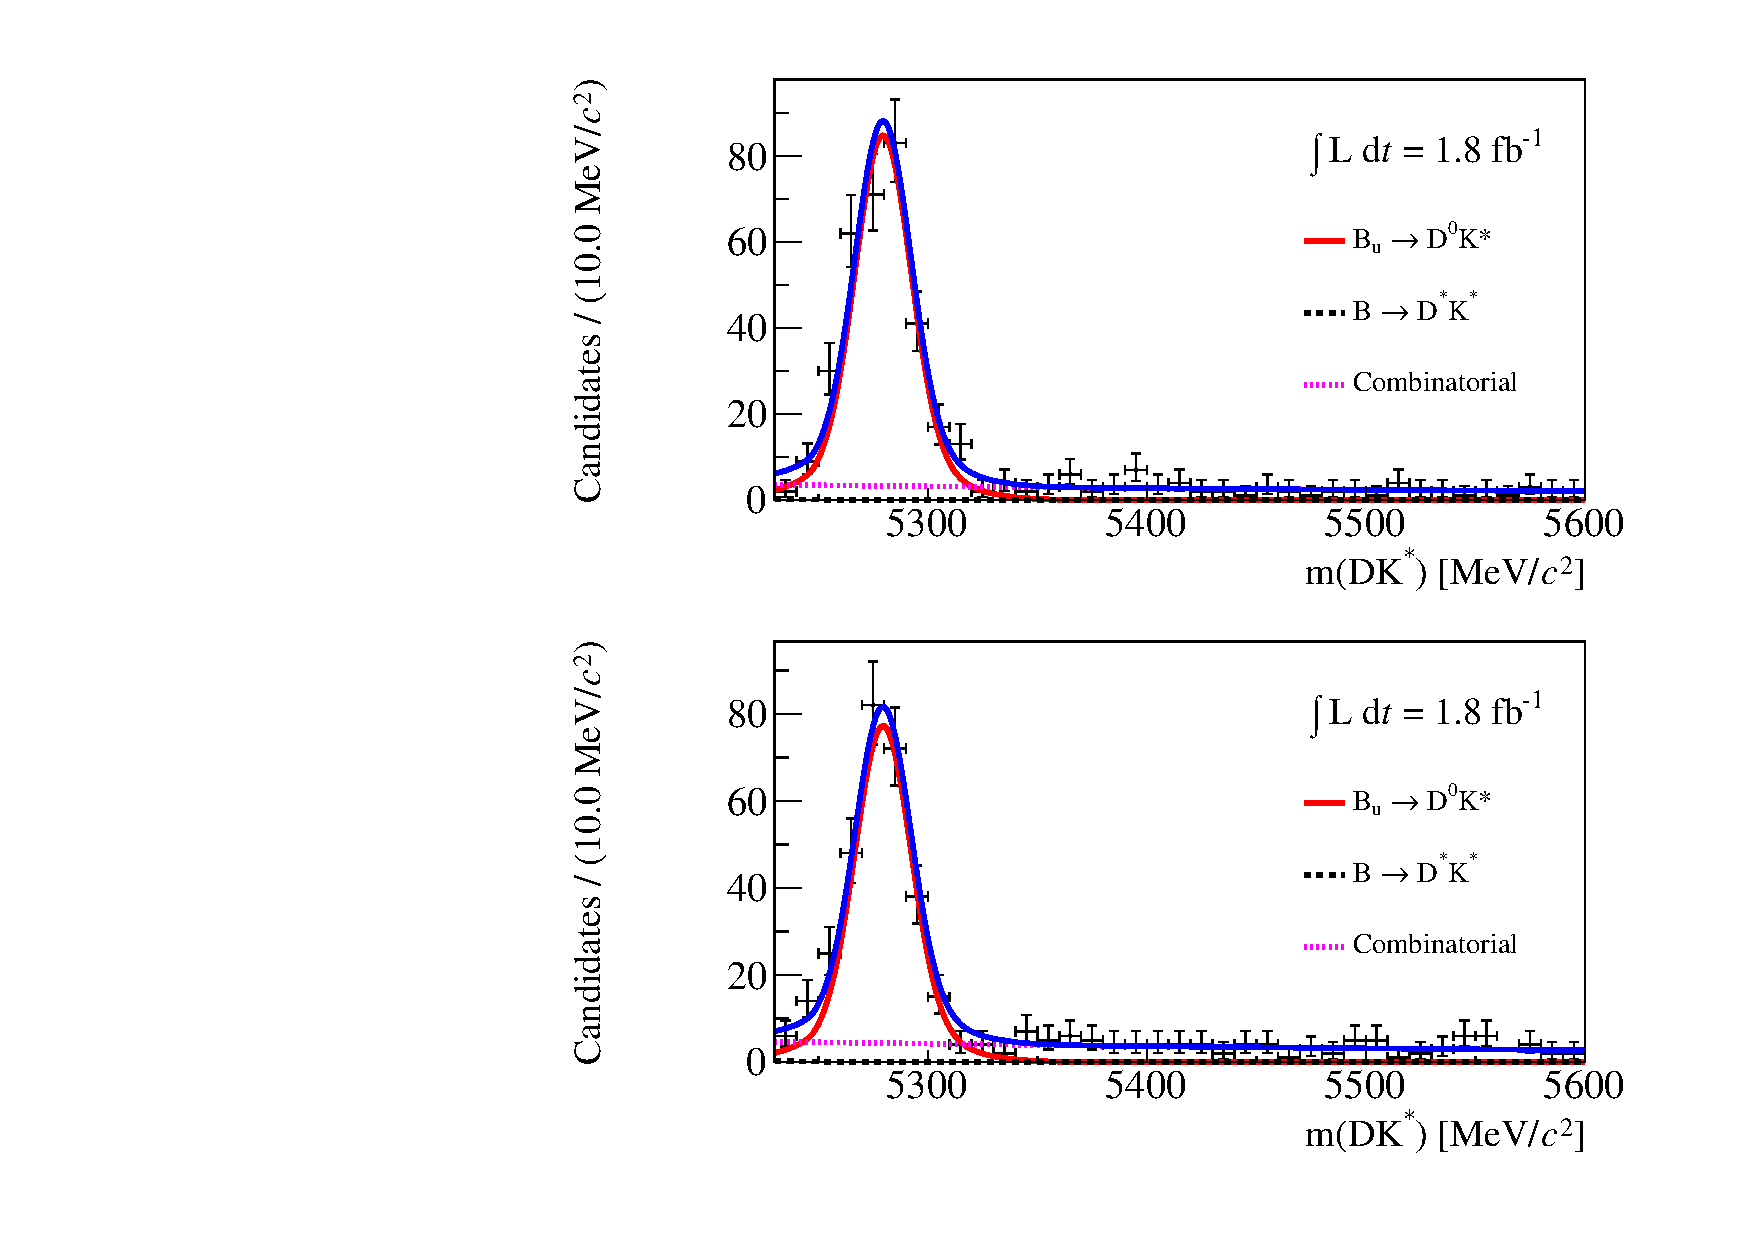
\includegraphics[width=0.3\linewidth]{figures/results/canvas_d2kpipipi_DD_run2.pdf}}
\hfill
\subfloat[$\pi\pi\pi\pi$, DD]{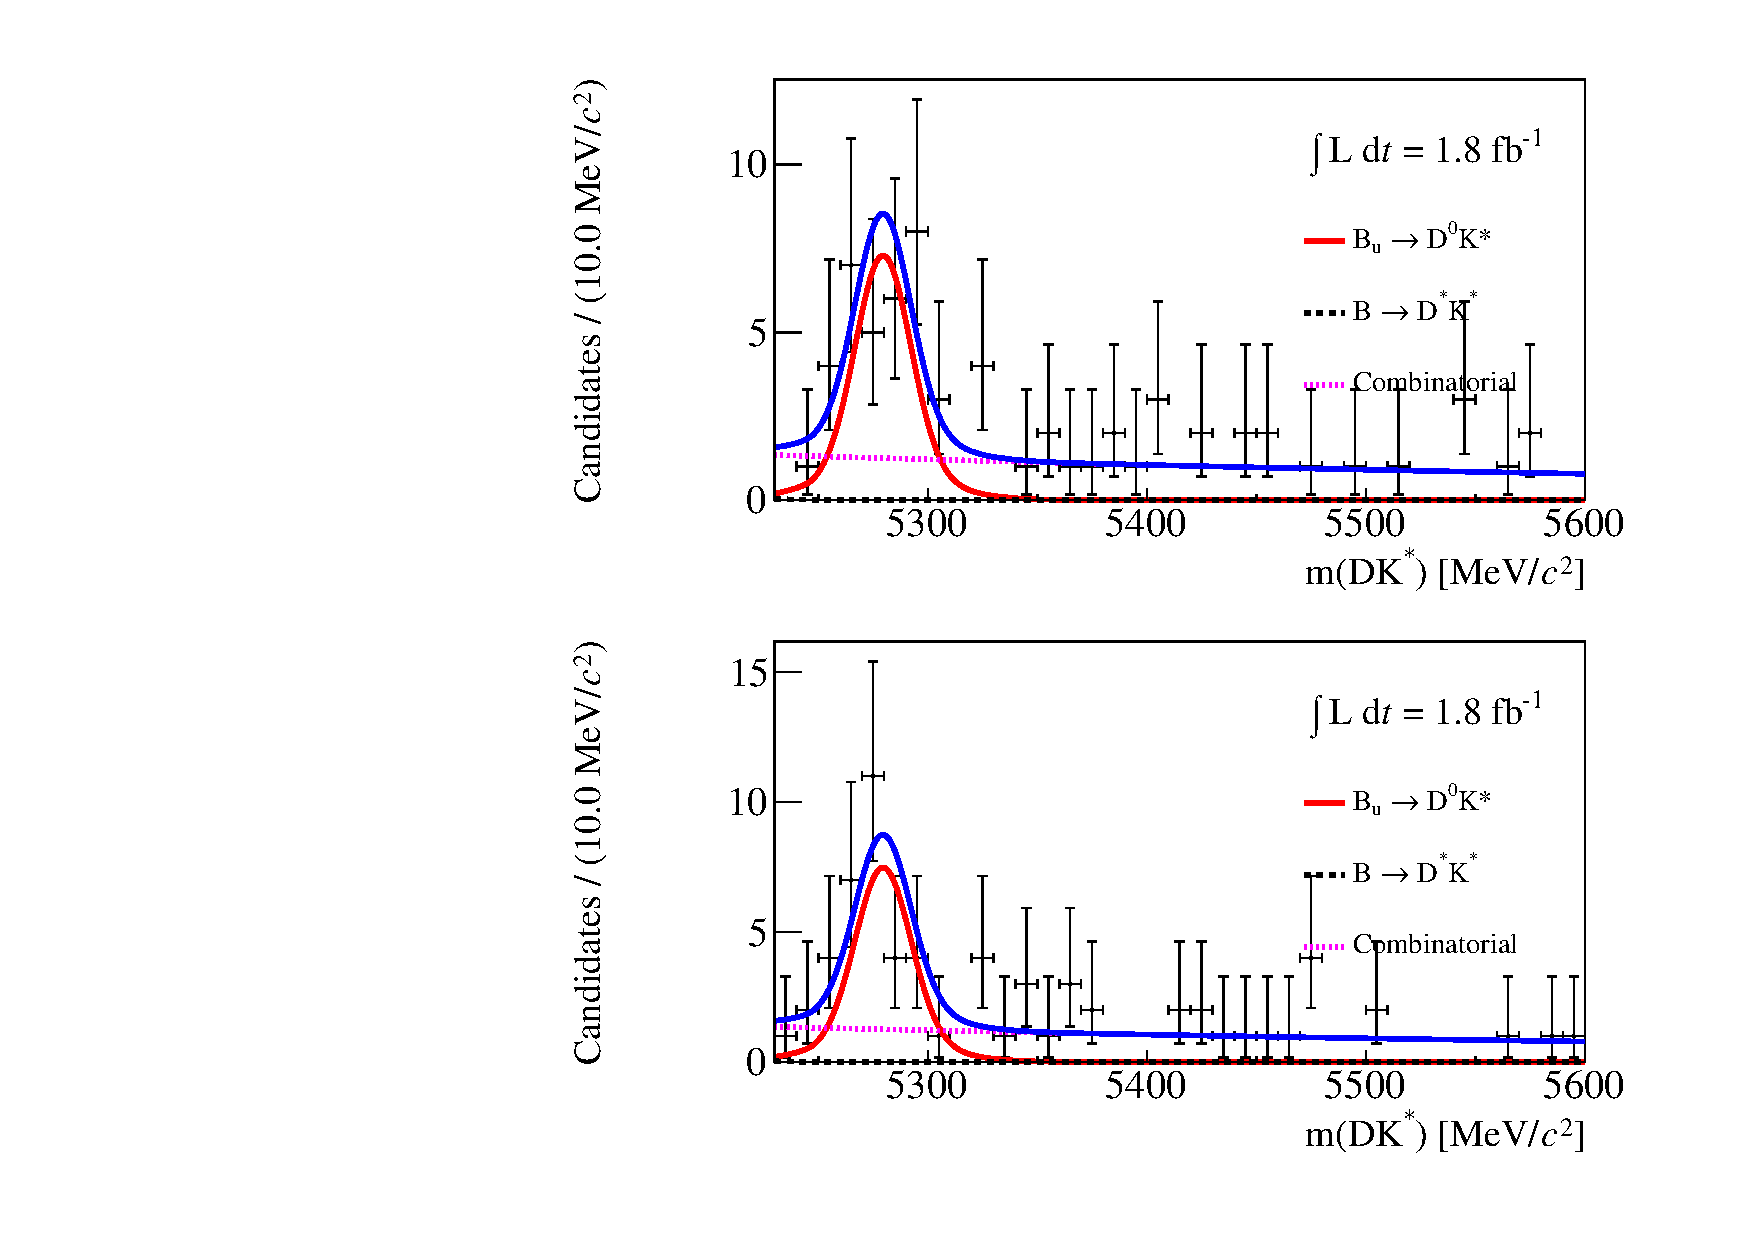
\includegraphics[width=0.3\linewidth]{figures/results/canvas_d2pipipipi_DD_run2.pdf}}
\hfill
\subfloat[$\pi K\pi\pi$, DD]{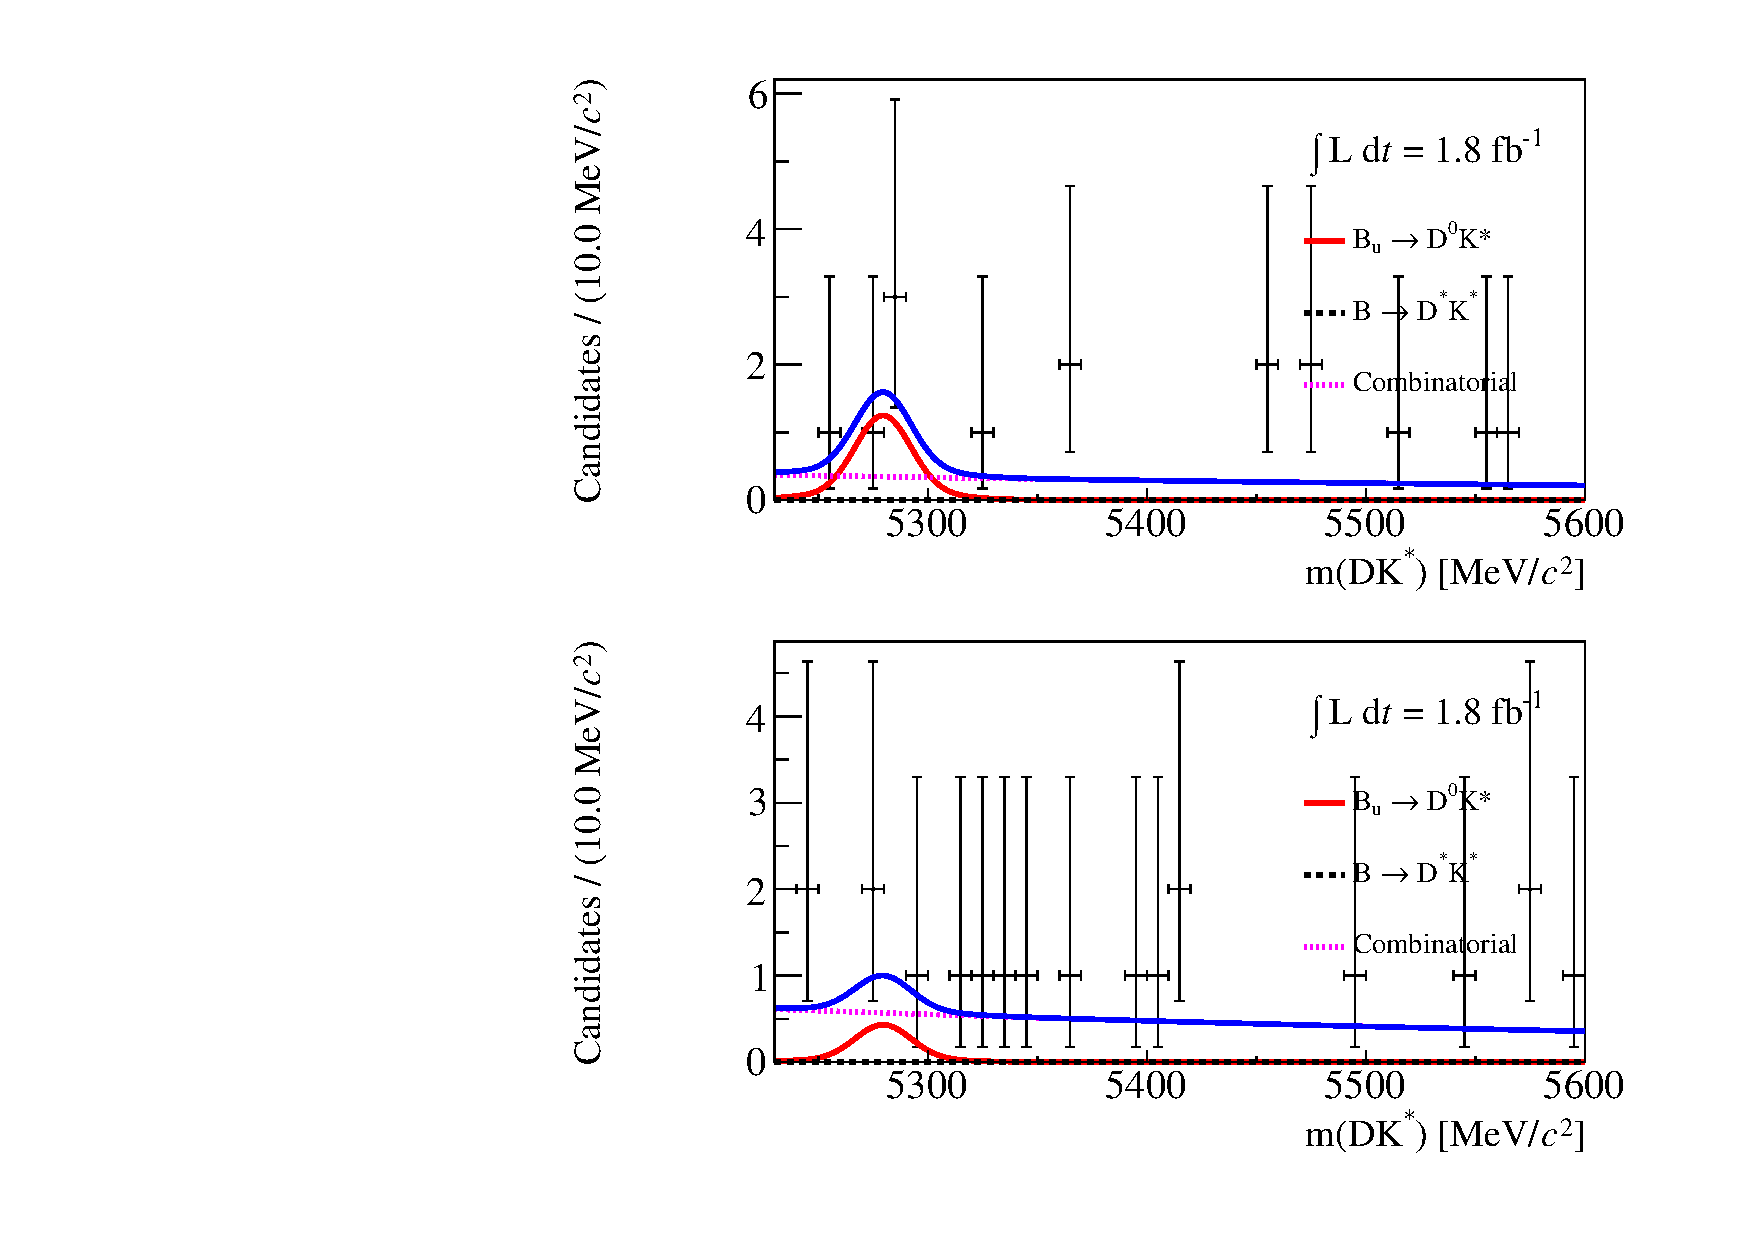
\includegraphics[width=0.3\linewidth]{figures/results/canvas_d2pikpipi_DD_run2.pdf}}
\caption{Results of the simultaneous fit for \runtwo data for four-body modes. In each pair the top plot is for \Bp decays and the bottom plot is for \Bm decays.}
\label{datafit4bodyRun2}
\end{sidewaysfigure}

\begin{table}[h]
\centering
{\footnotesize
\begin{tabular}{cccc}
Parameter & Fitted value & Negative error & Positive error \\
\hline
$A_{K\pi}$ & $-0.004$ & $-0.023$ & $0.023$ \\
$A_{KK}$ & $0.06$ & $-0.07$ & $0.07$ \\
$A_{\pi\pi}$ & $0.15$ & $-0.13$ & $0.13$ \\
$R_{KK}$ & $1.24$ & $-0.08$ & $0.09$ \\
$R_{\pi\pi}$ & $1.08$ & $-0.14$ & $0.15$ \\
$R^+_{K\pi}$ & $0.020$ & $-0.006$ & $0.006$ \\
$R^-_{K\pi}$ & $0.0018$ & $-0.0032$ & $0.0040$ \\
$A_{K\pi\pi\pi}$ & $-0.013$ & $-0.031$ & $0.031$ \\
$A_{\pi\pi\pi\pi}$ & $0.03$ & $-0.11$ & $0.11$ \\
$R_{\pi\pi\pi\pi}$ & $1.11$ & $-0.12$ & $0.13$ \\
$R^+_{K\pi\pi\pi}$ & $0.016$ & $-0.006$ & $0.008$ \\
$R^-_{K\pi\pi\pi}$ & $0.006$ & $-0.005$ & $0.006$ \\
\end{tabular}}
\caption{Fitted values of all the \CP parameters from the \CP fit.}
\label{cpfitresultsphysics}
\end{table}

\begin{table}[h]
\centering
{\footnotesize
\begin{tabular}{cccc}
Parameter & Fitted value & Negative error & Positive error \\
\hline
N\_d2kpi\_DD\_run1 & $503$ & $-22$ & $23$ \\
N\_d2kpi\_DD\_run2 & $911$ & $-32$ & $32$ \\
N\_d2kpi\_LL\_run1 & $228$ & $-14$ & $15$ \\
N\_d2kpi\_LL\_run2 & $388$ & $-19$ & $19$ \\
N\_d2kpipipi\_DD\_run1 & $233$ & $-15$ & $16$ \\
N\_d2kpipipi\_DD\_run2 & $560$ & $-26$ & $26$ \\
N\_d2kpipipi\_LL\_run1 & $101$ & $-9$ & $10$ \\
N\_d2kpipipi\_LL\_run2 & $251$ & $-16$ & $16$ \\
bu\_mean\_kpi & $5279.4$ & $-0.3$ & $0.3$ \\
bu\_mean\_kpipipi & $5279.5$ & $-0.5$ & $0.5$ \\
bu\_width\_kpi & $12.1$ & $-0.3$ & $0.3$ \\
bu\_width\_kpipipi & $12.6$ & $-0.4$ & $0.4$ \\
exp\_kpi\_DD\_combs\_slope & $-0.0008$ & $-0.0006$ & $0.0006$ \\
exp\_kpi\_LL\_combs\_slope & $0.0002$ & $-0.0011$ & $0.0012$ \\
exp\_kpipipi\_DD\_combs\_slope & $-0.0014$ & $-0.0006$ & $0.0006$ \\
exp\_kpipipi\_LL\_combs\_slope & $-0.0003$ & $-0.0014$ & $0.0015$ \\
\end{tabular}}
\caption{Fitted values of the signal yields and shape parameters from the \CP fit.}
\label{cpfitresultsshapes}
\end{table}

\begin{table}[h]
\centering
{\tiny
\begin{tabular}{cccc}
Parameter & Fitted value & Negative error & Positive error \\
\hline
n\_comb\_d2kk\_minus\_DD\_run1 & $9.2644$ & $-3.2413$ & $4.1306$ \\
n\_comb\_d2kk\_minus\_DD\_run2 & $29.5912$ & $-5.8248$ & $6.6312$ \\
n\_comb\_d2kk\_minus\_LL\_run1 & $0.0000$ & $0.0000$ & $0.8409$ \\
n\_comb\_d2kk\_minus\_LL\_run2 & $10.2769$ & $-3.2586$ & $4.0635$ \\
n\_comb\_d2kk\_plus\_DD\_run1 & $11.0377$ & $-3.2611$ & $4.0359$ \\
n\_comb\_d2kk\_plus\_DD\_run2 & $28.5043$ & $-5.6729$ & $6.4917$ \\
n\_comb\_d2kk\_plus\_LL\_run1 & $6.9477$ & $-2.7573$ & $3.6031$ \\
n\_comb\_d2kk\_plus\_LL\_run2 & $4.1843$ & $-1.9720$ & $2.8582$ \\
n\_comb\_d2kpi\_minus\_DD\_run1 & $54.6504$ & $-8.3230$ & $9.2240$ \\
n\_comb\_d2kpi\_minus\_DD\_run2 & $155.8847$ & $-14.5137$ & $15.4315$ \\
n\_comb\_d2kpi\_minus\_LL\_run1 & $7.9888$ & $-2.8410$ & $3.7060$ \\
n\_comb\_d2kpi\_minus\_LL\_run2 & $15.9239$ & $-4.2968$ & $5.2111$ \\
n\_comb\_d2kpi\_plus\_DD\_run1 & $64.6413$ & $-9.1168$ & $10.0035$ \\
n\_comb\_d2kpi\_plus\_DD\_run2 & $154.8678$ & $-14.5472$ & $15.4779$ \\
n\_comb\_d2kpi\_plus\_LL\_run1 & $13.0412$ & $-3.8827$ & $4.7734$ \\
n\_comb\_d2kpi\_plus\_LL\_run2 & $19.8632$ & $-4.8676$ & $5.7870$ \\
n\_comb\_d2kpipipi\_minus\_DD\_run1 & $43.3016$ & $-7.2924$ & $8.1779$ \\
n\_comb\_d2kpipipi\_minus\_DD\_run2 & $135.8805$ & $-13.5205$ & $14.4923$ \\
n\_comb\_d2kpipipi\_minus\_LL\_run1 & $1.2423$ & $-0.8669$ & $1.6936$ \\
n\_comb\_d2kpipipi\_minus\_LL\_run2 & $9.5762$ & $-3.1916$ & $4.1240$ \\
n\_comb\_d2kpipipi\_plus\_DD\_run1 & $26.9317$ & $-5.7903$ & $6.6844$ \\
n\_comb\_d2kpipipi\_plus\_DD\_run2 & $99.1967$ & $-11.8452$ & $12.8635$ \\
n\_comb\_d2kpipipi\_plus\_LL\_run1 & $3.2506$ & $-1.7378$ & $2.6474$ \\
n\_comb\_d2kpipipi\_plus\_LL\_run2 & $13.2367$ & $-3.9555$ & $4.9514$ \\
n\_comb\_d2pik\_minus\_DD\_run1 & $4.9988$ & $-1.9166$ & $2.5806$ \\
n\_comb\_d2pik\_minus\_DD\_run2 & $22.0339$ & $-4.6793$ & $5.3881$ \\
n\_comb\_d2pik\_minus\_LL\_run1 & $5.7087$ & $-2.1669$ & $2.8313$ \\
n\_comb\_d2pik\_minus\_LL\_run2 & $8.7460$ & $-2.6869$ & $3.3592$ \\
n\_comb\_d2pik\_plus\_DD\_run1 & $3.5811$ & $-1.7805$ & $2.5381$ \\
n\_comb\_d2pik\_plus\_DD\_run2 & $18.5923$ & $-4.4531$ & $5.1798$ \\
n\_comb\_d2pik\_plus\_LL\_run1 & $6.2716$ & $-2.3435$ & $3.0760$ \\
n\_comb\_d2pik\_plus\_LL\_run2 & $10.1699$ & $-3.0098$ & $3.7295$ \\
n\_comb\_d2pikpipi\_minus\_DD\_run1 & $2.3189$ & $-1.2711$ & $1.9952$ \\
n\_comb\_d2pikpipi\_minus\_DD\_run2 & $17.6630$ & $-4.0703$ & $4.7570$ \\
n\_comb\_d2pikpipi\_minus\_LL\_run1 & $2.8918$ & $-1.4152$ & $2.0824$ \\
n\_comb\_d2pikpipi\_minus\_LL\_run2 & $8.0364$ & $-2.7499$ & $3.4109$ \\
n\_comb\_d2pikpipi\_plus\_DD\_run1 & $8.5916$ & $-2.7559$ & $3.4576$ \\
n\_comb\_d2pikpipi\_plus\_DD\_run2 & $11.3239$ & $-3.2068$ & $3.9408$ \\
n\_comb\_d2pikpipi\_plus\_LL\_run1 & $0.5468$ & $0.0000$ & $1.5795$ \\
n\_comb\_d2pikpipi\_plus\_LL\_run2 & $8.1112$ & $-2.7664$ & $3.5289$ \\
n\_comb\_d2pipi\_minus\_DD\_run1 & $2.5555$ & $-1.3991$ & $2.1909$ \\
n\_comb\_d2pipi\_minus\_DD\_run2 & $22.3622$ & $-5.1858$ & $6.0198$ \\
n\_comb\_d2pipi\_minus\_LL\_run1 & $2.8497$ & $-1.5111$ & $2.2778$ \\
n\_comb\_d2pipi\_minus\_LL\_run2 & $4.5092$ & $-1.8921$ & $2.6286$ \\
n\_comb\_d2pipi\_plus\_DD\_run1 & $6.3000$ & $-2.4807$ & $3.2589$ \\
n\_comb\_d2pipi\_plus\_DD\_run2 & $20.7800$ & $-4.7887$ & $5.5926$ \\
n\_comb\_d2pipi\_plus\_LL\_run1 & $1.2180$ & $-0.8483$ & $1.6131$ \\
n\_comb\_d2pipi\_plus\_LL\_run2 & $4.4715$ & $-1.9438$ & $2.6960$ \\
n\_comb\_d2pipipipi\_minus\_DD\_run1 & $6.4229$ & $-2.4483$ & $3.2700$ \\
n\_comb\_d2pipipipi\_minus\_DD\_run2 & $39.6563$ & $-6.6510$ & $7.4336$ \\
n\_comb\_d2pipipipi\_minus\_LL\_run1 & $4.4140$ & $-1.9854$ & $2.7711$ \\
n\_comb\_d2pipipipi\_minus\_LL\_run2 & $14.1558$ & $-3.8758$ & $4.6747$ \\
n\_comb\_d2pipipipi\_plus\_DD\_run1 & $8.7170$ & $-3.0106$ & $3.8208$ \\
n\_comb\_d2pipipipi\_plus\_DD\_run2 & $38.6850$ & $-6.5763$ & $7.3661$ \\
n\_comb\_d2pipipipi\_plus\_LL\_run1 & $3.0998$ & $-1.4649$ & $2.1490$ \\
n\_comb\_d2pipipipi\_plus\_LL\_run2 & $9.5359$ & $-3.1792$ & $4.0340$ \\
\end{tabular}}
\caption{Fitted values of all the combinatoric yields from the \CP fit.}
\label{cpfitresultscomb}
\end{table}

\begin{table}
\centering
\begin{tabular}{c|c}
\hline
\D mode & Total yield \\
\hline
$K\pi$ & $2030 \pm 49$ \\
$KK$ & $257 \pm 18$ \\
$\pi\pi$ & $80 \pm 11$ \\
$\pi K$ & $20 \pm 7$ \\
$K\pi\pi\pi$ & $1144 \pm 37$ \\
$\pi\pi\pi\pi$ & $115 \pm 13$ \\
$\pi K\pi\pi$ & $13 \pm 7$ \\
\hline
\end{tabular}
\caption{Total fitted yields in each of the \Dz decay modes extracted from the simultaneous fit performed with \Bm and \Bp charges combined.}
\label{fittedyields}
\end{table}


%%%%%%%%%%%%%%%%%%%%%%%%

\clearpage

\section{Systematics}
\label{sec:systematics}

When performing the \CP fit, uncertainty in the \CP observables arises from statistical fluctuations in the data due to the limited size of the data sample. These uncertainties, shown in Table \ref{cpfitresultsphysics}, are referred to as statistical uncertainty. However, there is a different source of uncertainty arising from the assumptions involved in the construction and implementation of the model. These assumptions include those made about the shapes used to model different components in the fit, as described in Section \ref{sec:massfit}, and the use of fixed value inputs calculated prior to the fit, which have an associated uncertainty, as described in Section \ref{sec:cpfit:setup}. The uncertainties originating from assumptions made in the construction and implementation of the model are referred to as systematic uncertainties.

In this section, various sources of systematic uncertainty that affect the measurements of the \CP observables are investigated. Many fixed parameters are used in the fit model. Each of these fixed inputs has an associated uncertainty which needs to be propagated to the \CP observables giving rise to the systematic uncertainties. Uncertainties from the assumptions made for individual model components used in the \CP fit must also be propagated to the \CP observables. 
%Systematic uncertainties are computed either by multiple fits to data with certain parameters varied or by using pseudoexperiments where the generation is different to the fit model. 

\subsection{Sources of systematic uncertainty}

Branching fractions~\cite{PDG2016}, efficiencies and asymmetries are used as inputs to the \CP fit in order to relate the measured yields to the \CP observables, as described in Sections \ref{sec:cpfit:efficiencies} and \ref{sec:cpfit:asymmetries}. The systematic uncertainty for these fixed inputs is calculated based on how much the \CP observables are affected by changes to these inputs on the scale of their associated uncertainty. The systematic uncertainties due to the use of fixed inputs from branching ratios, simulation efficiencies, asymmetry corrections and shape parameters are estimated by performing multiple fits to data where each relevant parameter is varied according to a Gaussian distribution with the width as the assigned uncertainty. Any correlations between the parameters are ignored. Each time the fit is performed a value for each of the fitted parameters is extracted, resulting in a distribution for each \CP observable. The standard deviation of each of these distributions is taken to be the systematic uncertainty for that \CP observable. 

Other systematic uncertainties arise from the modelling of the signal and partially reconstructed backgrounds and the effect of any residual charmless \B decays, discussed in Section \ref{sec:backgrounds:charmless}. The systematic uncertainties from these sources are computed by generating pseudoexperiments, as described in Section \ref{sec:cpfit:fitterbias}. For each of these systematic effects being investigated, the generated model is varied to account for the corresponding model assumption. For example, for the systematic related to the signal shape, the shape generated in the pseudoexperiments to describe the signal component is changed compared to the nominal model. When the fit is performed on this generated data, any difference in the measured \CP observables, compared to the values generated, represents an uncertainty in these observables due to the choice of signal shape in the model. For each of these systematic effects, the systematic uncertainty on each observable is taken to be the difference between the mean of the fitted parameter distribution from pseudoexperiments and the generated value. 

Each of the sources of systematic uncertainty, from both fixed inputs and model components, is described individually in the following sections. A summary of the systematic uncertainties for the \CP observables is given in Table~\ref{systematics}.

\subsubsection{Branching ratios}

The branching ratios for the different \D decays are used in the \CP fit as shown in Equations \ref{effcorrectionglw2body} and \ref{effcorrectionglw4body}. The values used for the branching ratios are given in Table \ref{BR} along with their uncertainties. A systematic is assigned by performing 1000 fits to data each time varying the branching ratio values by a Gaussian with a width corresponding to the uncertainty of each branching ratio.

\begin{table}
\centering
\begin{tabular}{l|l}
\hline
Mode & Branching ratio \\
\hline
$\mathcal{B}(\decay{\Dz}{\Km\pip})$ & $0.0393 \pm 0.0004$ \\
$\mathcal{B}(\decay{\Dz}{\Kp\Km})$ & $0.00401 \pm 0.00007$ \\
$\mathcal{B}(\decay{\Dz}{\pip\pim})$ & $0.001421 \pm 0.000025$ \\
$\mathcal{B}(\decay{\Dz}{\Km\pip\pim\pip})$ & $0.0811 \pm 0.0015$ \\
$\mathcal{B}(\decay{\Dz}{\pip\pim\pip\pim})$ & $0.00745 \pm 0.00020$ \\
\hline
\end{tabular}
\caption{Branching ratios for the different \Dz decay modes, which are used as fixed inputs in the \CP fit~\cite{PDG2014}.}
\label{BR}
\end{table}


\subsubsection{Simulation efficiencies}

Selection efficiencies and BDT efficiencies are used in the \CP fit as shown in Equations \ref{effcorrectionglw2body}, \ref{effcorrectionglw4body}, \ref{effcorrectionads2body} and \ref{effcorrectionads4body}. The values used in the \CP fit are shown in Tables \ref{seleff} and \ref{bdteff} along with their uncertainties. These values are fixed in the \CP fit. A systematic is assigned by performing 1000 fits to data each time varying these fixed parameters according to a Gaussian whose width is the assigned uncertainty for that parameter.

\subsubsection{PID efficiencies}

PID efficiencies are used in the \CP fit as shown in Equations \ref{effcorrectionglw2body} and \ref{effcorrectionglw4body} and the values used are shown in Table \ref{pideff}. A systematic is assigned by performing 1000 fits to data each time varying the PID efficiencies according to a Gaussian whose width is the assigned uncertainty for that value.

\subsubsection{Veto efficiencies}

Veto efficiencies are required in the \CP fit to correct for the veto applied in the two- and four-body ADS modes, as shown in Equations \ref{effcorrectionads2body} and \ref{effcorrectionads4body}, with the actual values used shown in Table \ref{vetoeff} as well as the uncertainties. A systematic is assigned by performing 1000 fits to data each time varying the veto efficiencies according to a Gaussian whose width is the assigned uncertainty for that value.

\subsubsection{Asymmetry corrections}

Corrections must be made in the \CP for various sources of asymmetry as detailed in Section \ref{sec:cpfit:asymmetries}, namely production asymmetry, detection asymmetry and PID asymmetry. For each source of asymmetry a correction is applied in the \CP fit and a systematic is assigned separately to each based on the uncertainty of each correction. Details of the values used with their corresponding uncertainties are given in Section \ref{sec:cpfit:asymmetries}.

\subsubsection{Signal shape}
\label{sec:systematics:signal}

The signal shape, described in Section \ref{sec:massfit:signal}, is modelled as a Double Crystal Ball with all the parameters fixed from simulation apart from the mean and width. From simulated signal samples it can be seen that the signal shape has more than one characteristic width and a low mass tail. There are two sources of uncertainty in the choice of signal shape: the tail parameters, $\alpha$ and $n$, and the width ratio and yield fraction, $f_{\sigma}$ and $f_{cb}$, between the two CBs. These two sources of uncertainty are treated separately and combined. The uncertainty in the tail parameters is quantified by generating 1000 toys with an alternative signal shape. This shape is taken to have the same width ratio and yield fraction as the Double Crystal Ball used in the \CP fit. Other parameters are fixed from a fit to the simulated signal sample, shown in Figure \ref{signalshapesys}. The \CP fit is then performed to this data, generated with this alternative shape, using the nominal fit model.  The results from this method are given in the first row of Table \ref{signalshapeSystematics}.

\begin{figure}[h]
\centering
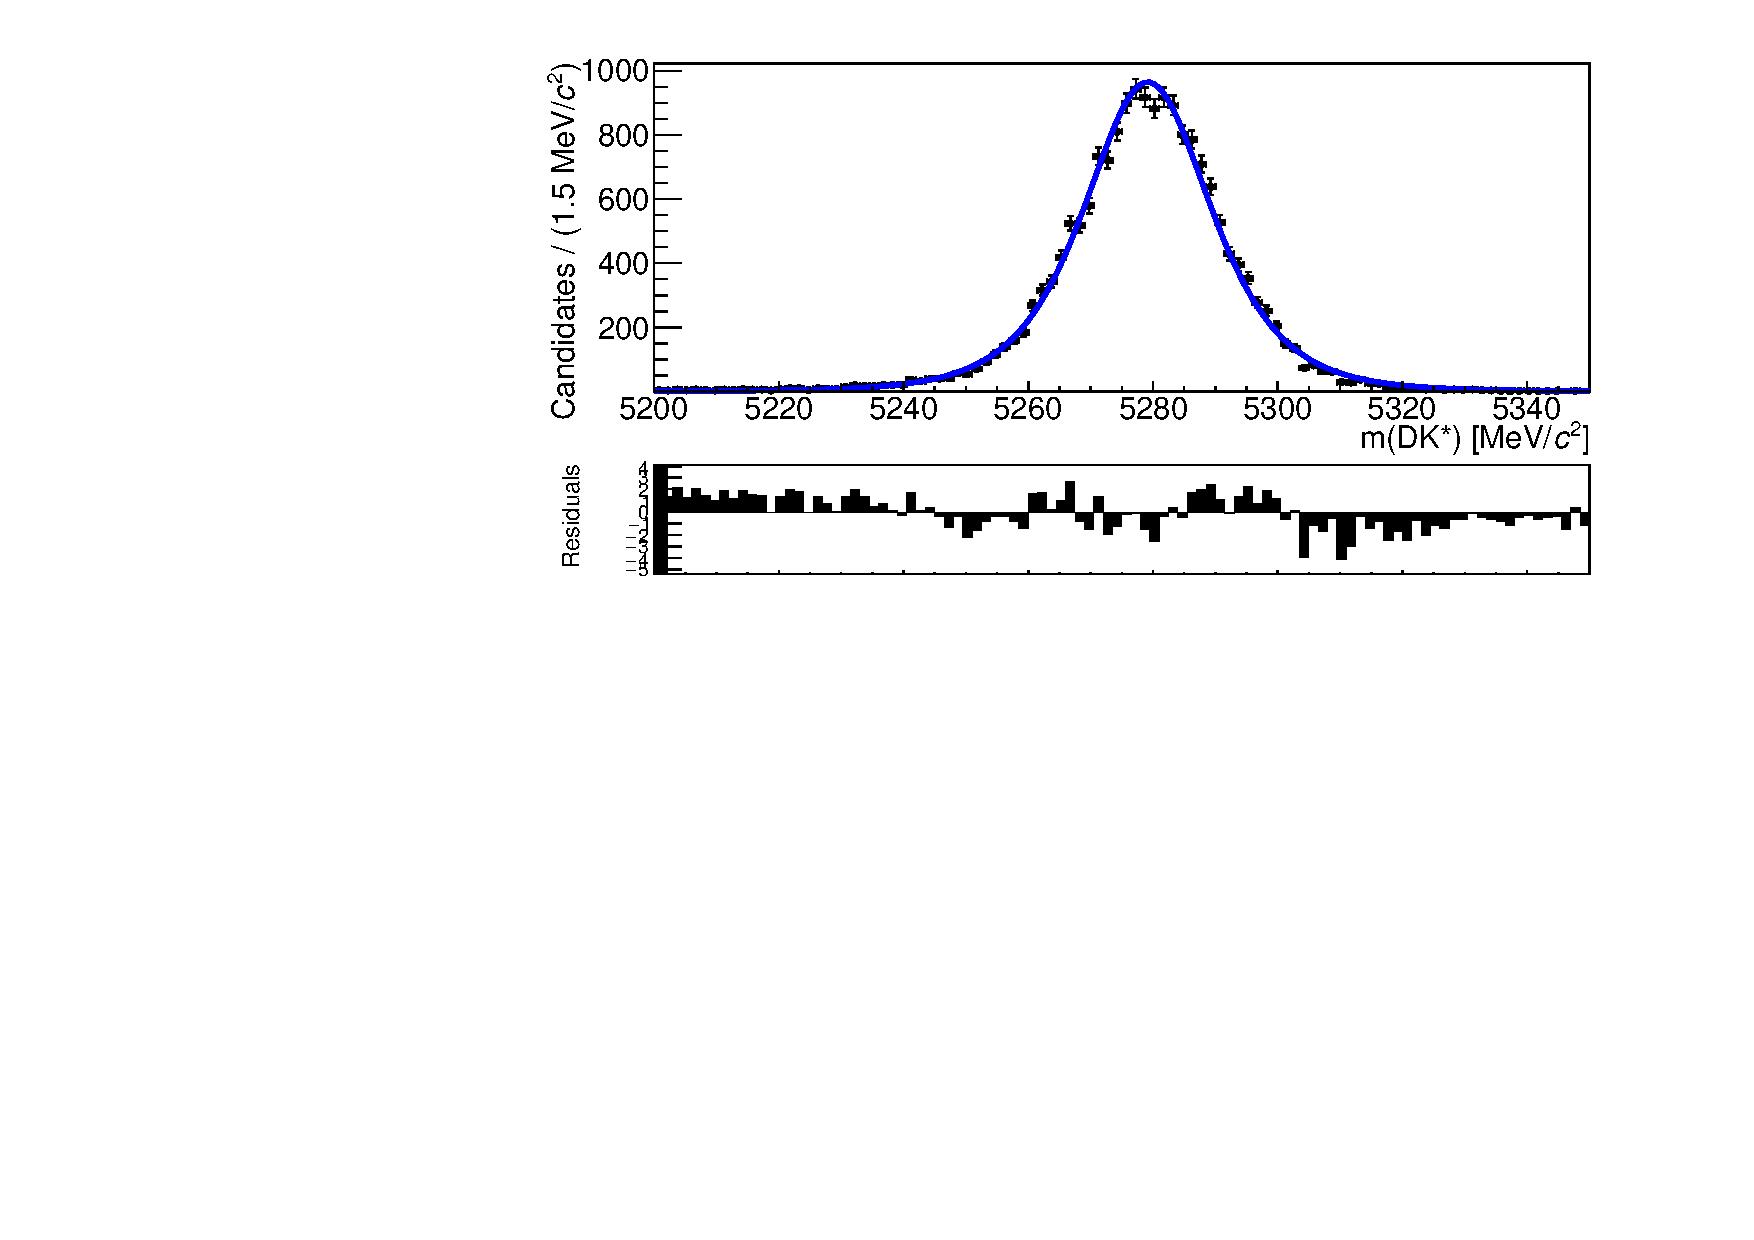
\includegraphics[width=0.5\linewidth]{figures/fitComponents/signalShape_DD_KPi_Johnson.pdf}
\caption{Fit performed on a simulated signal sample of DD candidates using an alternative shape.}
\label{signalshapesys}
\end{figure}

For the uncertainty in the width ratio and yield fraction, a systematic is assigned by performing 1000 fits to data each time varying the width ratio and yield fraction according to a Gaussian whose width is the assigned uncertainty for that value, which is taken from the fits to simulated samples, as given in Table \ref{signalparameters}. The results from this method are given in the second row of Table \ref{signalshapeSystematics}. The systematic from generating a Double Johnson distribution and that from varying the Double Crystal Ball parameters are added in quadrature to give the total signal shape systematic.

\begin{table}[h]
\centering
{\footnotesize
\resizebox{\textwidth}{!}{
\begin{tabular}{ccccccccc}
\hline
& $A_{K\pi}$ & $A_{KK}$ & $A_{\pi\pi}$ & $R_{KK}$ & $R_{\pi\pi}$ & $R^+_{K\pi}$ & $R^-_{K\pi}$ \\
\hline
Alternative shape & $1.1 \times 10^{-3}$ & $2.9 \times 10^{-3}$ & $1.1 \times 10^{-2}$ & $3.0 \times 10^{-3}$ & $2.6 \times 10^{-2}$ & $1.0 \times 10^{-3}$ & $1.3 \times 10^{-3}$ \\
Vary parameters & $2.3 \times 10^{-4}$ & $1.1 \times 10^{-3}$ & $1.4 \times 10^{-3}$ & $5.9 \times 10^{-4}$ & $4.4 \times 10^{-3}$ & $2.2 \times 10^{-4}$ & $1.1 \times 10^{-4}$ \\
\hline
Total & $1.1 \times 10^{-3}$ & $3.1 \times 10^{-3}$ & $1.1 \times 10^{-2}$ & $3.0 \times 10^{-2}$ & $2.7 \times 10^{-2}$ & $1.1 \times 10^{-3}$ & $1.3 \times 10^{-3}$ \\
\hline
\end{tabular}}
\begin{tabular}{cccccc}
\hline
& $A_{K\pi\pi\pi}$ & $A_{\pi\pi\pi\pi}$ & $R_{\pi\pi\pi\pi}$ & $R^+_{K3\pi}$ & $R^-_{K3\pi}$ \\
\hline
Alternative shape & $1.6 \times 10^{-3}$ & $1.3 \times 10^{-3}$ & $9.8 \times 10^{-3}$ & $3.0 \times 10^{-3}$ & $3.8 \times 10^{-3}$ \\
Vary parameters & $4.7 \times 10^{-4}$ & $1.8 \times 10^{-3}$ & $2.5 \times 10^{-3}$ & $2.4 \times 10^{-4}$ & $1.2 \times 10^{-4}$ \\
\hline
Total & $1.7 \times 10^{-3}$ & $2.2 \times 10^{-3}$ & $1.0 \times 10^{-2}$ & $3.0 \times 10^{-3}$ & $3.8 \times 10^{-3}$ \\
\hline
\end{tabular}}
\caption{Summary of systematic uncertainties associated with the signal shape.}
\label{signalshapeSystematics}
\end{table}

\subsubsection{Combinatoric background}

The shape parameter of the combinatoric, $\beta$, is fixed across all \Dz modes in the \CP fit, as there is not enough data for the fit to be stable if the shapes are allowed to vary in each mode. In order to get an idea of the variation in combinatoric shape between different \Dz modes, individual fits are performed to each \Dz decay mode in the high \Bm mass region (5400 - 5600 \mevcc) using an exponential function, as shown in Figures \ref{combinatoricLL} and \ref{combinatoricDD}. The data used for these fits is \runone data with the selection applied, except for \Kstar selection and \Dz and \KS FD significance cuts. PID selection on the \Dz daughters is applied in order to be sure of accessing the difference between the different \Dz modes. The looser selection requirements described result in enough data to perform a meaningful fit.

\begin{figure}[h]
\centering
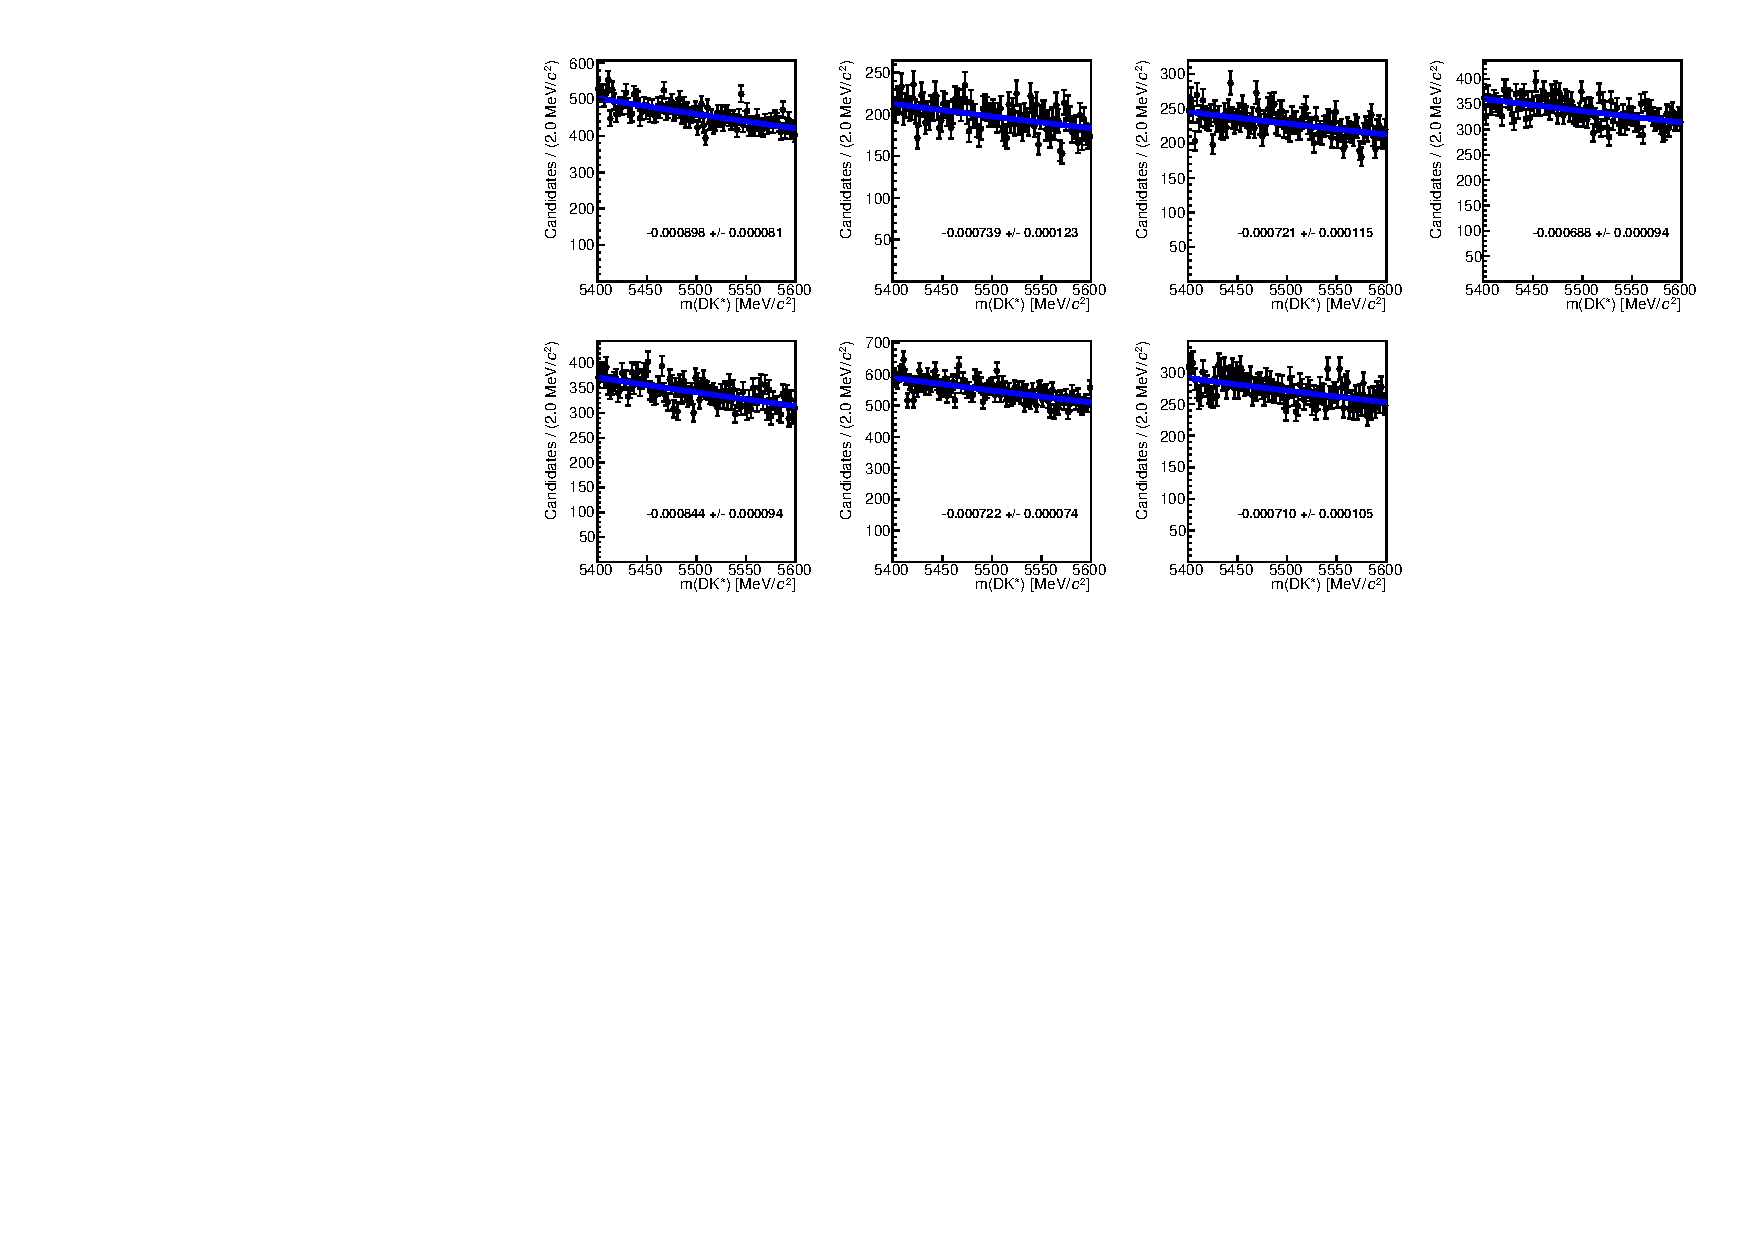
\includegraphics[width=\linewidth]{figures/fitComponents/combinatoricFits_LL.pdf}
\caption{Fits to the combinatoric background in the high \Bm mass region for LL candidates. The fitted values for the exponential slope parameter, $\beta$, are given on each plot.}
\label{combinatoricLL}
\end{figure}

\begin{figure}[h]
\centering
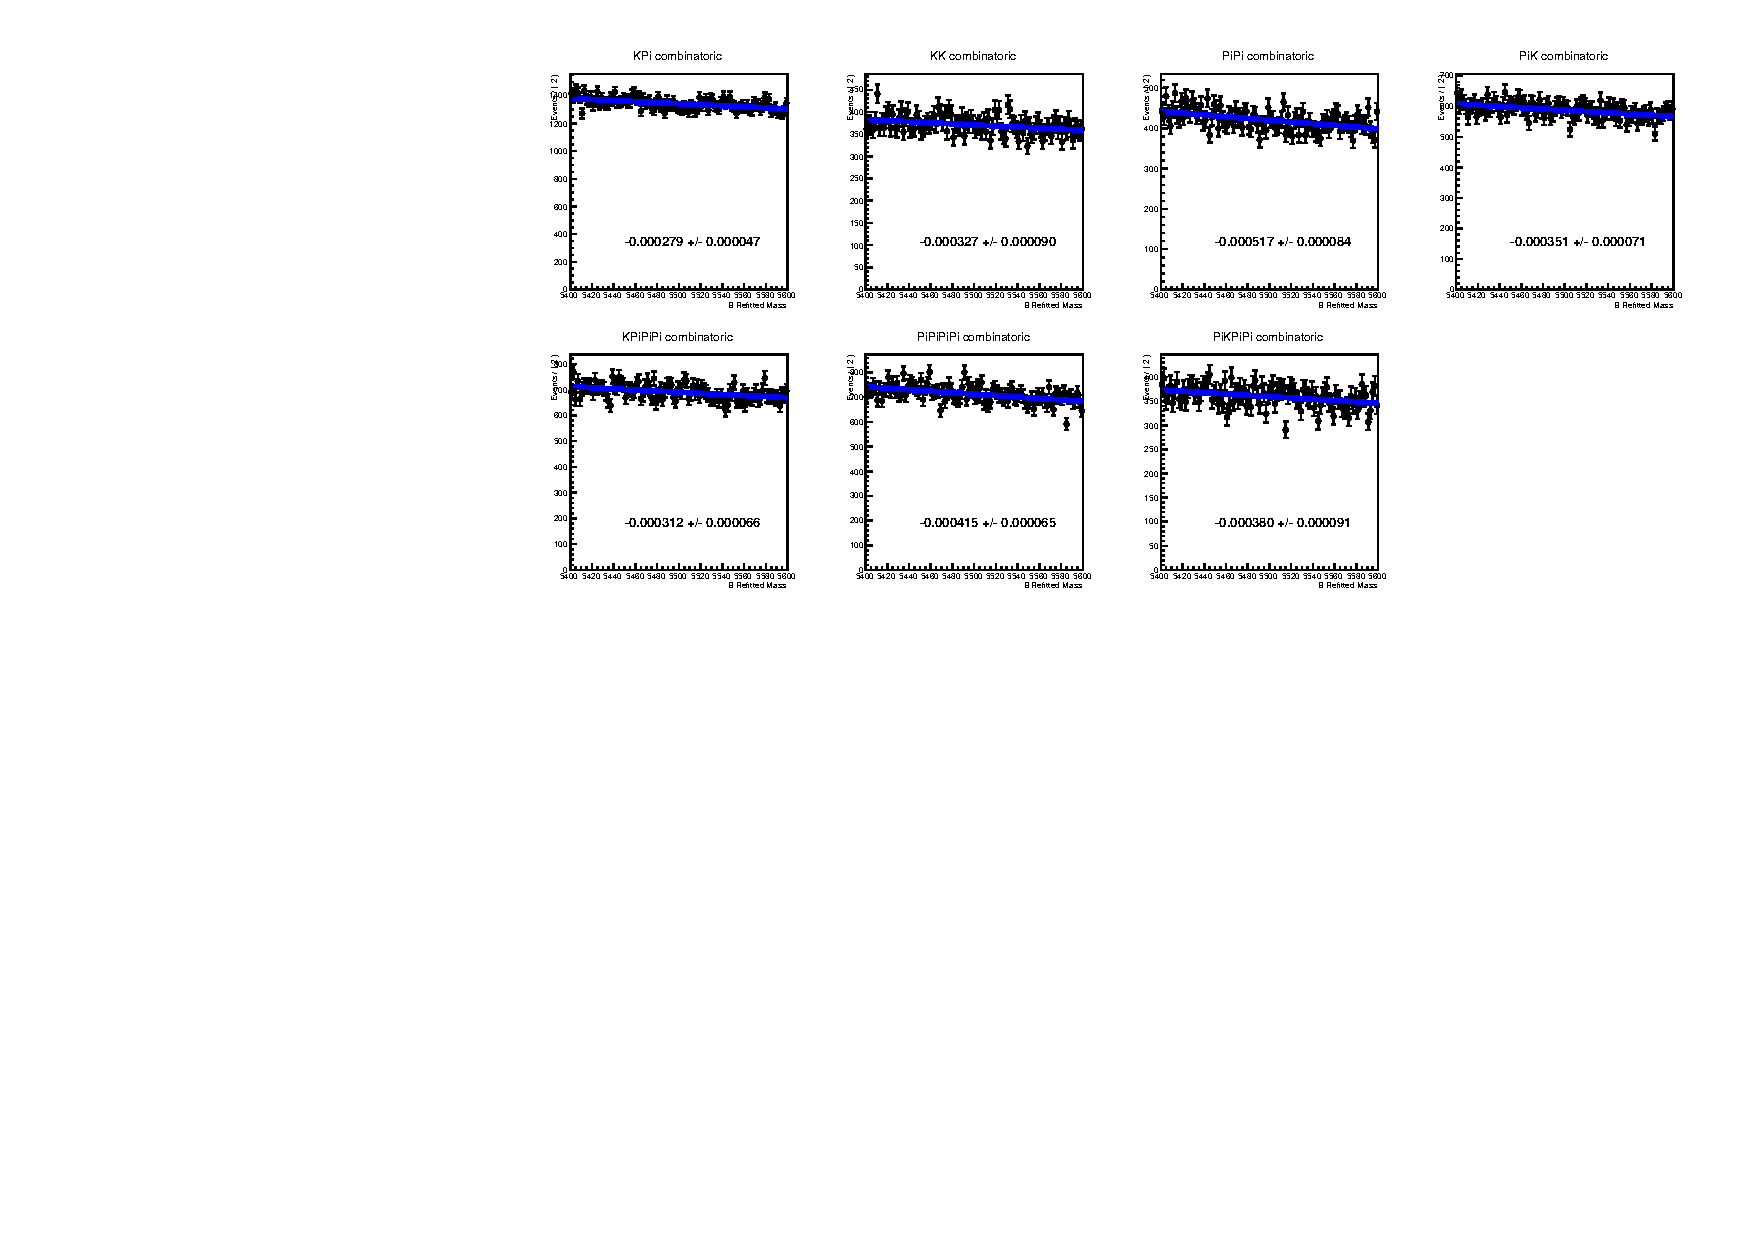
\includegraphics[width=\linewidth]{figures/fitComponents/combinatoricFits_DD.pdf}
\caption{Fits to the combinatoric background in the high \Bm mass region for DD candidates. The fitted values for the exponential slope parameter, $\beta$, are given on each plot.}
\label{combinatoricDD}
\end{figure}

The systematic is assigned by generating 1000 pseudoexperiments with the combinatoric slope parameter, $\beta$, for each \Dz mode fixed to those given in Figures \ref{combinatoricLL} and \ref{combinatoricDD}. The fit is then performed to this generated data using the nominal fit model.

\subsubsection{Partially reconstructed background}
\label{sec:systematics:partreco}

The partially reconstructed decays have a completely fixed shape and yield contributing to the \CP fit. The shape parameters are fixed from fits to simulated samples, yield ratios are fixed from branching ratios and simulation efficiencies and total yield is fixed from the fit to \kpi invariant mass, as described in Section \ref{sec:massfit:partreco}. The estimated yield is divided equally between \Bp and \Bm bins. In order to assign a systematic uncertainty, three different modifications are made to the partially reconstructed region, when generating samples for pseudoexperiments. These modifications are:

\begin{itemize}
\item The yield is increased by 20\%. The uncertainty in the yield from the fit to \kpi invariant mass is about 5\%, but this is considered to be an underestimate, therefore a conservative systematic of 20\% is used,
\item All partially reconstructed shapes are smeared by the difference in signal width between simulated samples and data. The width for all partially reconstructed shapes is increased by 4\% of LL bins and 5\% for DD bins,
\item A 10\% asymmetry is introduced for the partially reconstructed shapes.
\end{itemize}

These adjustments are applied simultaneously. The systematic uncertainty is assigned by generating 1000 pseudoexperiments with the above modifications implemented. The fit is then performed to this generated data using the nominal fit model.

\subsubsection{Charmless}

Section \ref{sec:backgrounds:charmless} shows that there is a possibility for residual charmless contribution to be present in \pipi mode. In order to estimate the systematic uncertainty associated with this possible charmless contribution, charmless events in the \pipi mode were generated according to a Gaussian whose mean is the expected number of charmless events and the width is the corresponding uncertainty. This expected value is rounded to a whole number and randomly distributed between \Bp and \Bm as an additional contribution to the yield in the signal region. The systematic is assigned by generating 1000 pseudoexperiments with a charmless contribution introduced. The fit is then performed to this generated data using the nominal fit model. The difference between the generated values of the \CP observables and the distribution obtained from the fits quantifies the effect of the possible charmless contamination on the measurement of the \CP observables.

\subsubsection{\boldmath \decay{\Lb}{\Lc(p\kaon\pi)\Kstarm} background}

The model for the \kk mass spectrum in \CP fit contains an additional background from \decay{\Lb}{\Lc(p\kaon\pi)\Kstarm}, as described in Section \ref{sec:backgrounds:Lb2LcKst}. The shape parameters are fixed from a fit to a simulated sample of \decay{\Lb}{\Lc(p\kaon\pi)\Km}, the values of which are given in Table \ref{fitresultsLb}. The systematic uncertainty corresponding to this model component is estimated by performing 1000 fits to data each time varying the shape parameters according to a Gaussian whose width is the assigned uncertainty for that value.

\subsubsection{\boldmath \decay{\Bs}{\Dzb\bar{K}^{*}(1410)^0} background}

The decay \decay{\Bs}{\Dzb\bar{K}^{*}(1410)^0} is considered as a background for the ADS mode, as described in Section \ref{sec:backgrounds:bs}. The shape is taken from a fit to simulated events and the yield is estimated to be $2.6 \pm 2.6$. The systematic uncertainty for any possible contamination from this background is estimated by performing 1000 fits to data each time varying the yield according to a Gaussian with a mean and width corresponding to the estimated yield.

\subsection{Results of systematic uncertainties}

Table \ref{systematics} summarises the systematic uncertainties for each of the different sources discussed in this section. If the systematic uncertainty was found to be more than two orders of magnitude smaller than the statistical uncertainty then a value of zero is given. Systematics from simulation efficiencies and branching ratios mainly affects \Rkk and \Rpipi. Production and detection asymmetry systematics contribute to \Akpi, \Akk and \Apipi. Systematic uncertainty from PID efficiencies do not contribute much to the systematic uncertainty. PID asymmetry corrections are found to be negligible; they do not contribute enough to be included in Table \ref{systematics}. The signal shape systematic has a non-negligible effect on the uncertainty for all the \CP observables. All systematic uncertainties are smaller than the corresponding statistical uncertainty. 

\begin{sidewaystable}[htbp]
\centering
{\footnotesize
\begin{tabular}{ccccccccccccc} 
\hline	
%\rule{0pt}{4ex}
\rule{0pt}{2.5ex}\rule[-1.2ex]{0pt}{0ex} & $A_{K\pi}$ & $A_{KK}$ & $A_{\pi\pi}$ & $R_{KK}$ & $R_{\pi\pi}$ & $R^+_{K\pi}$ & $R^-_{K\pi}$ & $A_{K\pi\pi\pi}$ & $A_{\pi\pi\pi\pi}$ & $R_{\pi\pi\pi\pi}$ & $R^+_{K\pi\pi\pi}$ & $R^-_{K\pi\pi\pi}$ \\
\hline
Statistical & $0.023$ & $0.07$ & $0.13$ & $0.09$ & $0.15$ & $0.006$ & $0.004$ & $0.031$ & $0.11$ & $0.13$ & $0.008$ & $0.007$ \\
\hline
Branching fractions & $-$ & $-$ & $0.013$ & $0.001$ & $0.012$ & $-$ & $-$ & $-$ & $0.0008$ & $0.027$ & $-$ & $-$ \\
Selection efficiencies  & $-$ & $-$ & $0.007$ & $-$ & $0.006$ & $0.0002$ & $-$ & $-$ & $0.0008$ & $0.014$ & $-$ & $-$ \\
PID efficiencies  & $-$ & $-$ & $0.002$ & $-$ & $0.002$ & $-$ & $-$ & $-$ & $-$ & $0.002$ & $-$ & $-$ \\
Veto efficiencies  & $-$ & $-$ & $-$ & $-$ & $-$ & $0.0001$ & $-$ & $-$ & $-$ & $-$ & $-$ & $-$ \\
$A_{\text{prod}}$  & $0.0073$ & $0.007$ & $-$ & $0.008$ & $-$ & $-$ & $-$ & $0.0079$ & $0.0077$ & $-$ & $-$ & $-$ \\
$A_{\text{det}}$  & $0.0034$ & $0.003$ & $-$ & $0.003$ & $-$ & $0.0001$ & $-$ & $0.0034$ & $0.0030$ & $-$ & $0.0001$ & $-$ \\
Signal shape & $0.0011$ & $0.003$ & $0.011$ & $0.003$ & $0.027$ & $0.0011$ & $0.0013$ & $0.0017$ & $0.0022$ & $0.010$ & $0.0030$ & $0.0038$ \\
Combinatorial shape  & $0.0012$ & $0.003$ & $0.004$ & $0.005$ & $0.009$ & $0.0002$ & $0.0003$ & $0.0001$ & $0.0018$ & $-$ & $0.0012$ & $0.0004$ \\
Partially reconstructed shape  & $0.0007$ & $0.001$ & $0.001$ & $0.003$ & $0.005$ & $-$ & $0.0003$ & $0.0003$ & $0.0005$ & $0.002$ & $0.0008$ & $0.0001$ \\
Charmless  & $0.0008$ & $-$ & $0.002$ & $0.003$ & $0.007$ & $-$ & $0.0003$ & $0.0009$ & $0.0030$ & $0.002$ & $0.0008$ & $0.0001$ \\
\decay{\Lb}{\Lc\Kstarm} & $0.0002$ & $-$ & $0.011$ & $-$ & $0.001$ & $0.0001$ & $-$ & $-$ & $-$ & $-$ & $-$ & $-$ \\
\decay{\Bs}{\D\Kstar(1410)^0} & $-$ & $-$ & $-$ & $-$ & $-$ & $0.0005$ & $0.0001$ & $-$ & $-$ & $-$ & $-$ & $-$ \\
\hline
Total systematic & $0.0083$ & $0.009$ & $0.022$ & $0.012$ & $0.032$ & $0.0012$ & $0.0014$ & $0.0088$ & $0.0093$ & $0.032$ & $0.0034$ & $0.0038$ \\
\hline
\end{tabular}}
\caption{Summary of systematic uncertainties. Uncertainties are not shown if they are more than two orders of magnitude smaller than the statistical uncertainty.}
\label{systematics}
\end{sidewaystable}

\section{Summary of results}
\label{sec:cpfit:summary}

The final results for the \CP observables, determined from the \CP fit performed in Section \ref{sec:cpfit:results}, are  
\begin{alignat*}{13}
A_{K\pi} &= &\ -&0.004&\ &\pm&\ &0.023&\ &\pm&\ &0.008& \\
A_{KK} &= &&0.06&\ &\pm&\ &0.07&\ &\pm&\ &0.01& \\
A_{\pi\pi} &= &&0.15&\ &\pm&\ &0.13&\ &\pm&\ &0.02& \\
R_{KK} &= &&1.22&\ &\pm&\ &0.09&\ &\pm&\ &0.01& \\
R_{\pi\pi} &= &&1.08&\ &\pm&\ &0.14&\ &\pm&\ &0.03& \\
R^+_{K\pi} &= &&0.020&\ &\pm&\ &0.006&\ &\pm&\ &0.001& \\ 
R^-_{K\pi} &= &&0.002&\ &\pm&\ &0.004&\ &\pm&\ &0.001& \\
A_{K\pi\pi\pi} &= &\ -&0.013&\ &\pm&\ &0.031&\ &\pm&\ &0.009& \\
A_{\pi\pi\pi\pi} &= &&0.02&\ &\pm&\ &0.11&\ &\pm&\ &0.01& \\
R_{\pi\pi\pi\pi} &= &&1.08&\ &\pm&\ &0.13&\ &\pm&\ &0.03& \\
R^+_{K\pi\pi\pi} &= &&0.016&\ &\pm&\ &0.007&\ &\pm&\ &0.003& \\ 
R^-_{K\pi\pi\pi} &= &&0.006&\ &\pm&\ &0.006&\ &\pm&\ &0.004&
\end{alignat*}
where the first uncertainty is statistical and the second is systematic. The correlation matrices for the statistical and systematic uncertainties are given in Tables~\ref{statisticalcorrelations} and \ref{systematiccorrelations}, respectively. The large correlations of the systematic uncertainties are mainly due to contributions from production and detection asymmetries. Combined results from the \Kp\Km and \pip\pim decay modes, taking correlations into account, are
\begin{alignat*}{13}
R_{\CP+} &= &\ &1.18&\ &\pm&\ &0.08&\ &\pm&\ &0.01& \\
A_{\CP+} &= &\ &0.08&\ &\pm&\ &0.06&\ &\pm&\ &0.01&
\end{alignat*}
where the first uncertainty is statistical and the second is systematic. In addition, $R^+$ and $R^-$ for the \Kp\pim and \Kp\pim\pip\pim decay modes can be transformed into the more commonly used $R_{ADS} = \left(R^- + R^+\right)/2\ $and \mbox{$A_{ADS} = \left(R^- - R^+\right)/\left(R^- + R^+\right)$}. These results, taking correlations into account, are
\begin{alignat*}{13}
R_{ADS}^{K\pi} &= &\ &0.011&\ &\pm&\ &0.004&\ &\pm&\ &0.001& \\
A_{ADS}^{K\pi} &= &\ -&0.81&\ &\pm&\ &0.17&\ &\pm&\ &0.04& \\
R_{ADS}^{K\pi\pi\pi} &= &\ &0.011&\ &\pm&\ &0.005&\ &\pm&\ &0.003& \\
A_{ADS}^{K\pi\pi\pi} &= &\ -&0.45&\ &\pm&\ &0.21&\ &\pm&\ &0.14&
\end{alignat*}
where the first uncertainty is statistical and the second is systematic. The measured asymmetries and ratios for the two-body \Dz meson decay modes are consistent with, and more precise than, the previous measurements from \babar~\cite{BaBarDKstar}.

\begin{table}[htbp]
\centering
{\scriptsize
\resizebox{\textwidth}{!}{
\begin{tabular}{c|cccccccccccc} 
\hline 
\rule{0pt}{2.5ex}\rule[-1.2ex]{0pt}{0ex}& $A_{K\pi}$ & $A_{KK}$ & $A_{\pi\pi}$ & $R_{KK}$ & $R_{\pi\pi}$ & $R^+_{K\pi}$ & $R^-_{K\pi}$ & $A_{K\pi\pi\pi}$ & $A_{\pi\pi\pi\pi}$ & $R_{\pi\pi\pi\pi}$ & $R^+_{K\pi\pi\pi}$ & $R^-_{K\pi\pi\pi}$ \\ 
 \hline
$A_{K\pi}$ & 1 & $-$ & $-$ & $-$ & $-$ & 0.08 & $-$0.01{\color{white}$-$} & $-$ & $-$ & $-$ & $-$ & $-$ \\
$A_{KK}$ & & 1 & $-$ & $-$ & $-$ & $-$ & $-$ & $-$ & $-$ & $-$ & $-$ & $-$ \\
$A_{\pi\pi}$ & & & 1 & $-$ & $-$0.02{\color{white}$-$} & $-$ & $-$ & $-$ & $-$ & $-$ & $-$ & $-$ \\
$R_{KK}$ & & & & 1 & 0.05 & 0.02 & $-$0.01{\color{white}$-$} & $-$ & $-$ & $-$ & $-$ & $-$ \\
$R_{\pi\pi}$ & & & & & 1 & 0.03 & 0.02 & $-$ & $-$ & $-$ & $-$ & $-$ \\
$R^+_{K\pi}$ & & & & & & 1 & 0.02 & $-$ & $-$ & $-$ & $-$ & $-$ \\
$R^-_{K\pi}$ & & & & & & & 1 & $-$ & $-$ & $-$ & $-$ & $-$ \\
$A_{K\pi\pi\pi}$ & & & & & & & & 1 & $-$ & $-$ & 0.07 & $-$0.03{\color{white}$-$} \\
$A_{\pi\pi\pi\pi}$ & & & & & & & & & 1 & 0.01 & $-$ & $-$ \\
$R_{\pi\pi\pi\pi}$ & & & & & & & & & & 1 & 0.04 & 0.04 \\
$R^+_{K\pi\pi\pi}$ & & & & & & & & & & & 1 & 0.03 \\
\rule[-1.2ex]{0pt}{0ex}$R^-_{K\pi\pi\pi}$ & & & & & & & & & & & & 1 \\
\hline 
\end{tabular}}}
\caption{Correlation matrix of the statistical uncertainties for the twelve physics observables from the simultaneous fit to data. Only half of the symmetric matrix is shown.}
\label{statisticalcorrelations}
\end{table}

\begin{table}[htbp]
\centering
{\scriptsize
\resizebox{\textwidth}{!}{
\begin{tabular}{c|cccccccccccc} 
\hline 
\rule{0pt}{2.5ex}\rule[-1.2ex]{0pt}{0ex}& $A_{K\pi}$ & $A_{KK}$ & $A_{\pi\pi}$ & $R_{KK}$ & $R_{\pi\pi}$ & $R^+_{K\pi}$ & $R^-_{K\pi}$ & $A_{K\pi\pi\pi}$ & $A_{\pi\pi\pi\pi}$ & $R_{\pi\pi\pi\pi}$ & $R^+_{K\pi\pi\pi}$ & $R^-_{K\pi\pi\pi}$ \\ 
 \hline
$A_{K\pi}$ & 1 & 0.82 & $-$ & 0.72 & $-$ & 0.01 & $-$0.02{\color{white}$-$} & 0.94 & 0.84 & $-$ & $-$0.01{\color{white}$-$} & $-$ \\
$A_{KK}$ & & 1 & $-$0.04{\color{white}$-$} & 0.65 & 0.02 & 0.01 & $-$0.02{\color{white}$-$} & 0.83 & 0.77 & $-$ & $-$ & $-$\\
$A_{\pi\pi}$ & & & 1 & $-$ & $-$ & 0.05 & 0.03 & $-$0.01{\color{white}$-$} & $-$ & $-$0.01{\color{white}$-$} & $-$0.01{\color{white}$-$} & $-$0.01{\color{white}$-$} \\
$R_{KK}$ & & & & 1 & $-$0.03{\color{white}$-$} & $-$ & $-$0.02{\color{white}$-$} & 0.72 & 0.68 & $-$ & $-$ & 0.01 \\
$R_{\pi\pi}$ & & & & & 1 & 0.06 & 0.08 & $-$0.01{\color{white}$-$} & $-$ & $-$0.01{\color{white}$-$} & $-$0.02{\color{white}$-$} & 0.01 \\
$R^+_{K\pi}$ & & & & & & 1 & 0.08 & $-$0.01{\color{white}$-$} & $-$ & $-$ & $-$0.01{\color{white}$-$} & $-$0.01{\color{white}$-$} \\
$R^-_{K\pi}$ & & & & & &  & 1 & $-$0.01{\color{white}$-$} & $-$0.01{\color{white}$-$} & $-$0.01{\color{white}$-$} & 0.01 & 0.03 \\
$A_{K\pi\pi\pi}$ & & & & & & & & 1 & 0.84 & $-$ & $-$0.01{\color{white}$-$} & $-$0.02{\color{white}$-$} \\
$A_{\pi\pi\pi\pi}$ & & & & & & & & & 1 & 0.03 & 0.01 & $-$ \\
$R_{\pi\pi\pi\pi}$ & & & & & & & & & & 1 & 0.01 & $-$0.01{\color{white}$-$} \\
$R^+_{K\pi\pi\pi}$ & & & & & & & & & & & 1 & 0.05 \\
\rule[-1.2ex]{0pt}{0ex}$R^-_{K\pi\pi\pi}$ & & & & & & & & & & & & 1 \\
\hline 
\end{tabular}}}
\caption{Correlation matrix of the systematic uncertainties for the twelve physics observables from the simultaneous fit to data. Only half of the symmetric matrix is shown.}
\label{systematiccorrelations}
\end{table}


\clearpage

